\label{3.5 C6S Answer Key}
\subsection{Answer Key}
\tiny
\renewcommand{\insertclass}{- Class 6}
\renewcommand{\insertsubject}{ - Science}

\begin{frame}[shrink=0.1,label=QPC6QC6S02 - DT - Q7]{Q28 [1. Components of Food]}
\vspace{-0.2cm}
\mcqtextbottomTwoTwo{
  questionnumber={28}, 
  questiontext={What is the purpose of including dietary fibre in our diet?},
  optionA={To provide energy to the body.},
  optionB={To support healthy digestion.},
  optionC={To improve the taste of food.},
  optionD={To reduce blood pressure.},
  questionTag={C6S02 - DT – Q7}, 
  correctoption={B},
}

\begin{minipage}{\linewidth}
\hspace{1cm}
\centering
\tiny
\renewcommand{\arraystretch}{1.25}
\begin{tabular}{|M{1.2cm}|M{0.8cm}|M{0.8cm}|M{0.8cm}|M{0.8cm}|M{0.8cm}|}
\hline
Option & A (\ding{55}) & \cellcolor{cellgreen} B (\ding{51}) & C (\ding{55}) & D (\ding{55}) & E \\ 
\hline
6 A & \highno{40\%} & \highno{53\%} & \highno{7\%} & \highno{0\%} & \highno{0\%} \\ 
 \hline 
6 B & \highno{42\%} & \highred{32\%} & \highno{21\%} & \highno{5\%} & \highno{0\%} \\ \hline
\end{tabular}
\end{minipage}

\end{frame}
% \input{4. PPT/6. My Answer/Science/C6/117_C6S - Q28}


\begin{frame}[shrink=0.1,label=QPC6QC6S02 - DT - Q4]{Q30 [1. Components of Food]}
\vspace{-0.2cm}
\mcqtextbottomOneFour{
  questionnumber={30}, 
  questiontext={Observe the given food items and identify the type of nutrient they are rich in.\\Milk, Egg, Fish, Groundnut, Soya beans},
  optionA={Fat},
  optionB={Minerals},
  optionC={Carbohydrate},
  optionD={Protein},
  questionTag={C6S02 - DT – Q4}, 
  correctoption={D},
}

\begin{minipage}{\linewidth}
\hspace{1cm}
\centering
\tiny
\renewcommand{\arraystretch}{1.25}
\begin{tabular}{|M{1.2cm}|M{0.8cm}|M{0.8cm}|M{0.8cm}|M{0.8cm}|M{0.8cm}|}
\hline
Option & A (\ding{55}) & B (\ding{55}) & C (\ding{55}) & \cellcolor{cellgreen} D (\ding{51}) & E \\ 
\hline
6 A & \highno{7\%} & \highno{13\%} & \highno{20\%} & \highno{60\%} & \highno{0\%} \\ 
 \hline 
6 B & \highno{11\%} & \highno{11\%} & \highno{5\%} & \highno{74\%} & \highno{0\%} \\ \hline
\end{tabular}
\end{minipage}

\end{frame}
% \input{4. PPT/6. My Answer/Science/C6/117_C6S - Q30}


\begin{frame}[shrink=0.1,label=QPC6QC6S02 - DT - Q18]{Q35 [1. Components of Food]}
\vspace{-0.2cm}

\mcqtextbottomOneFour{
  questionnumber={35}, 
  questionTag={C6S02 – DT – Q18}, 
  questiontext={Since Deva is overweight, the doctor advised him to eat less rice. This is because rice is high in \rule{80pt}{0.5pt}.},
  optionA={Protein},
  optionB={Fat},
  optionC={Vitamin},
  optionD={Carbohydrate},
  correctoption={D},
}


\begin{minipage}{\linewidth}
\hspace{1cm}
\centering
\tiny
\renewcommand{\arraystretch}{1.25}
\begin{tabular}{|M{1.2cm}|M{0.8cm}|M{0.8cm}|M{0.8cm}|M{0.8cm}|M{0.8cm}|}
\hline
Option & A (\ding{55}) & B (\ding{55}) & C (\ding{55}) & \cellcolor{cellgreen} D (\ding{51}) & E \\ 
\hline
6 A & \highno{0\%} & \highno{47\%} & \highno{20\%} & \highred{33\%} & \highno{0\%} \\ 
 \hline 
6 B & \highno{5\%} & \highno{42\%} & \highno{16\%} & \highred{37\%} & \highno{0\%} \\ \hline
\end{tabular}
\end{minipage}

\end{frame}
% \input{4. PPT/6. My Answer/Science/C6/117_C6S - Q35}


\begin{frame}[shrink=0.1,label=QPC6QC6S02 - DT - Q16]{Q59 [1. Components of Food]}
\vspace{-0.2cm}

\matextbottomOneFour{
myanswerquestion={Answer the following questions based on the churning process.},
myanswercontent={
\begin{minipage}{0.6\textwidth} 
List the products that we get after churning the curd. \vspace{0.5cm} \\ 
1. \rule{120pt}{0.5pt} \vspace{0.5cm} \\ 
2. \rule{120pt}{0.5pt} \\
\end{minipage}
\hfill
\begin{minipage}{0.3\textwidth} 
 {\adjustbox{scale=\scalefactor}{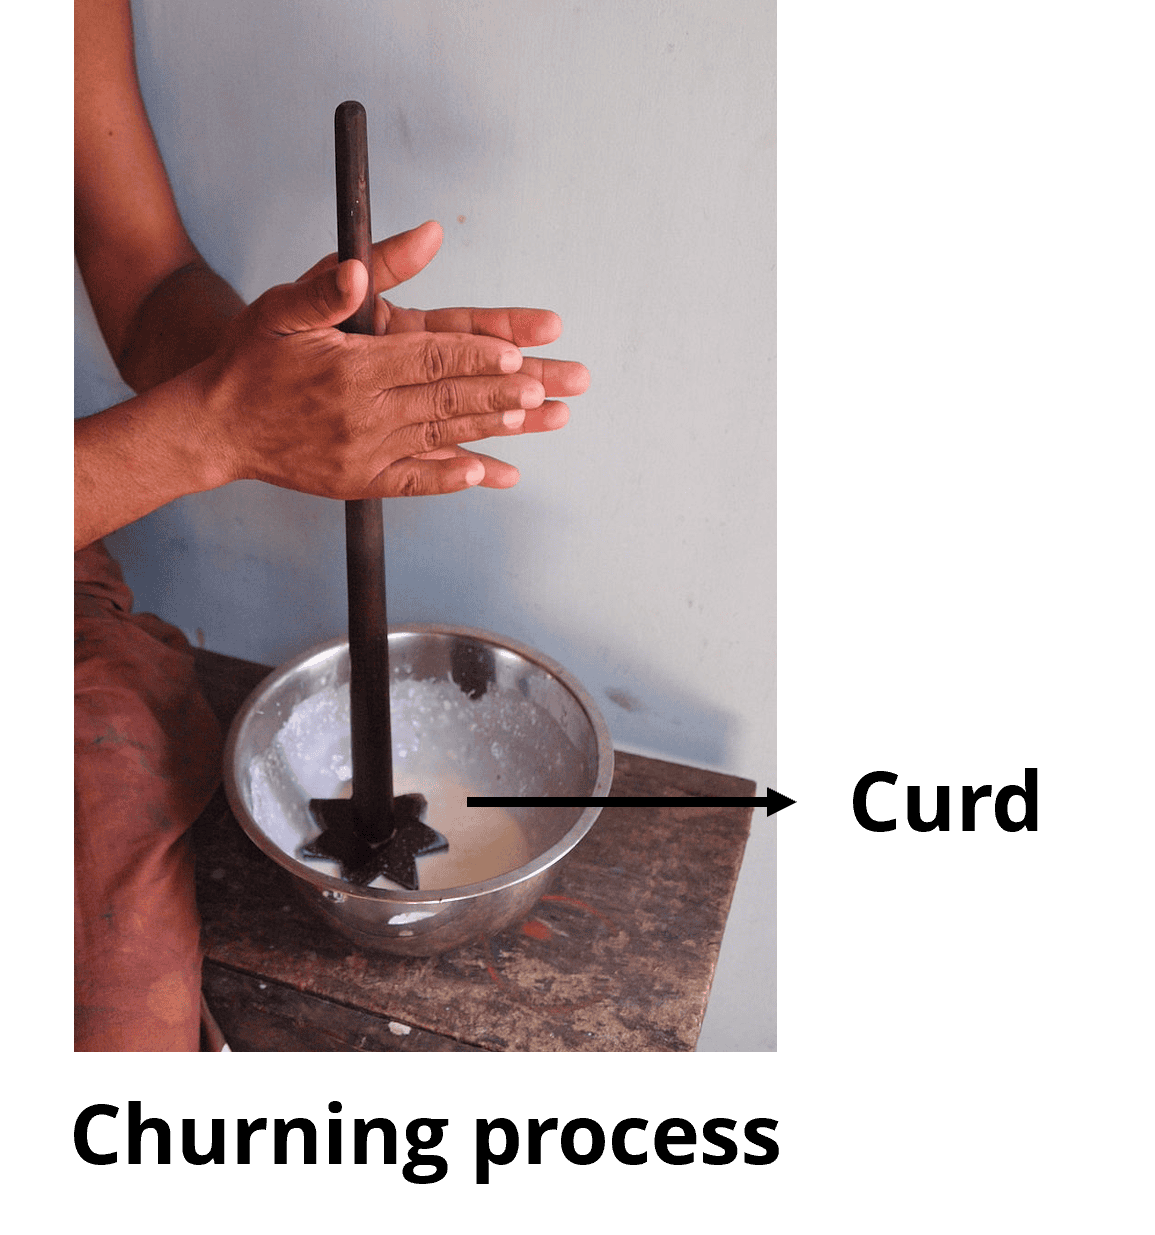
\includegraphics[width=4.5cm,height=4cm]{C6S02 - DT - Q16.png}}}
\end{minipage}
},
questionnumber={59}, 
questionTag={C6S02 - DT – Q16},
questiontext={After churning the curd, two different products are obtained. Identify the product that is rich in fat.},
optionA={Butter milk},
optionB={Butter},
optionC={Curd},
optionD={Water}, 
correctoption={B},
}


\begin{minipage}{\linewidth}
\hspace{1cm}
\centering
\tiny
\renewcommand{\arraystretch}{1.25}
\begin{tabular}{|M{1.2cm}|M{0.8cm}|M{0.8cm}|M{0.8cm}|M{0.8cm}|M{0.8cm}|}
\hline
Option & A (\ding{55}) & \cellcolor{cellgreen} B (\ding{51}) & C (\ding{55}) & D (\ding{55}) & E \\ 
\hline
6 A & \highno{27\%} & \highno{67\%} & \highno{7\%} & \highno{0\%} & \highno{0\%} \\ 
 \hline 
6 B & \highno{42\%} & \highred{37\%} & \highno{16\%} & \highno{5\%} & \highno{0\%} \\ \hline
\end{tabular}
\end{minipage}

\end{frame}
\begin{frame}{Q59 - My Answer Responses}
    \vspace{-0.6cm}
    \begin{multicols}{2}

    % Image: Q59_D117140_Science.png - Scaled height: 5.35mm
    \begin{minipage}{\linewidth}
    \RaggedRight\textbf{\tiny \highgreen{Sabarish B [B]}} \\ 
    \vspace{4.00pt}\fcolorbox{blue}{white}{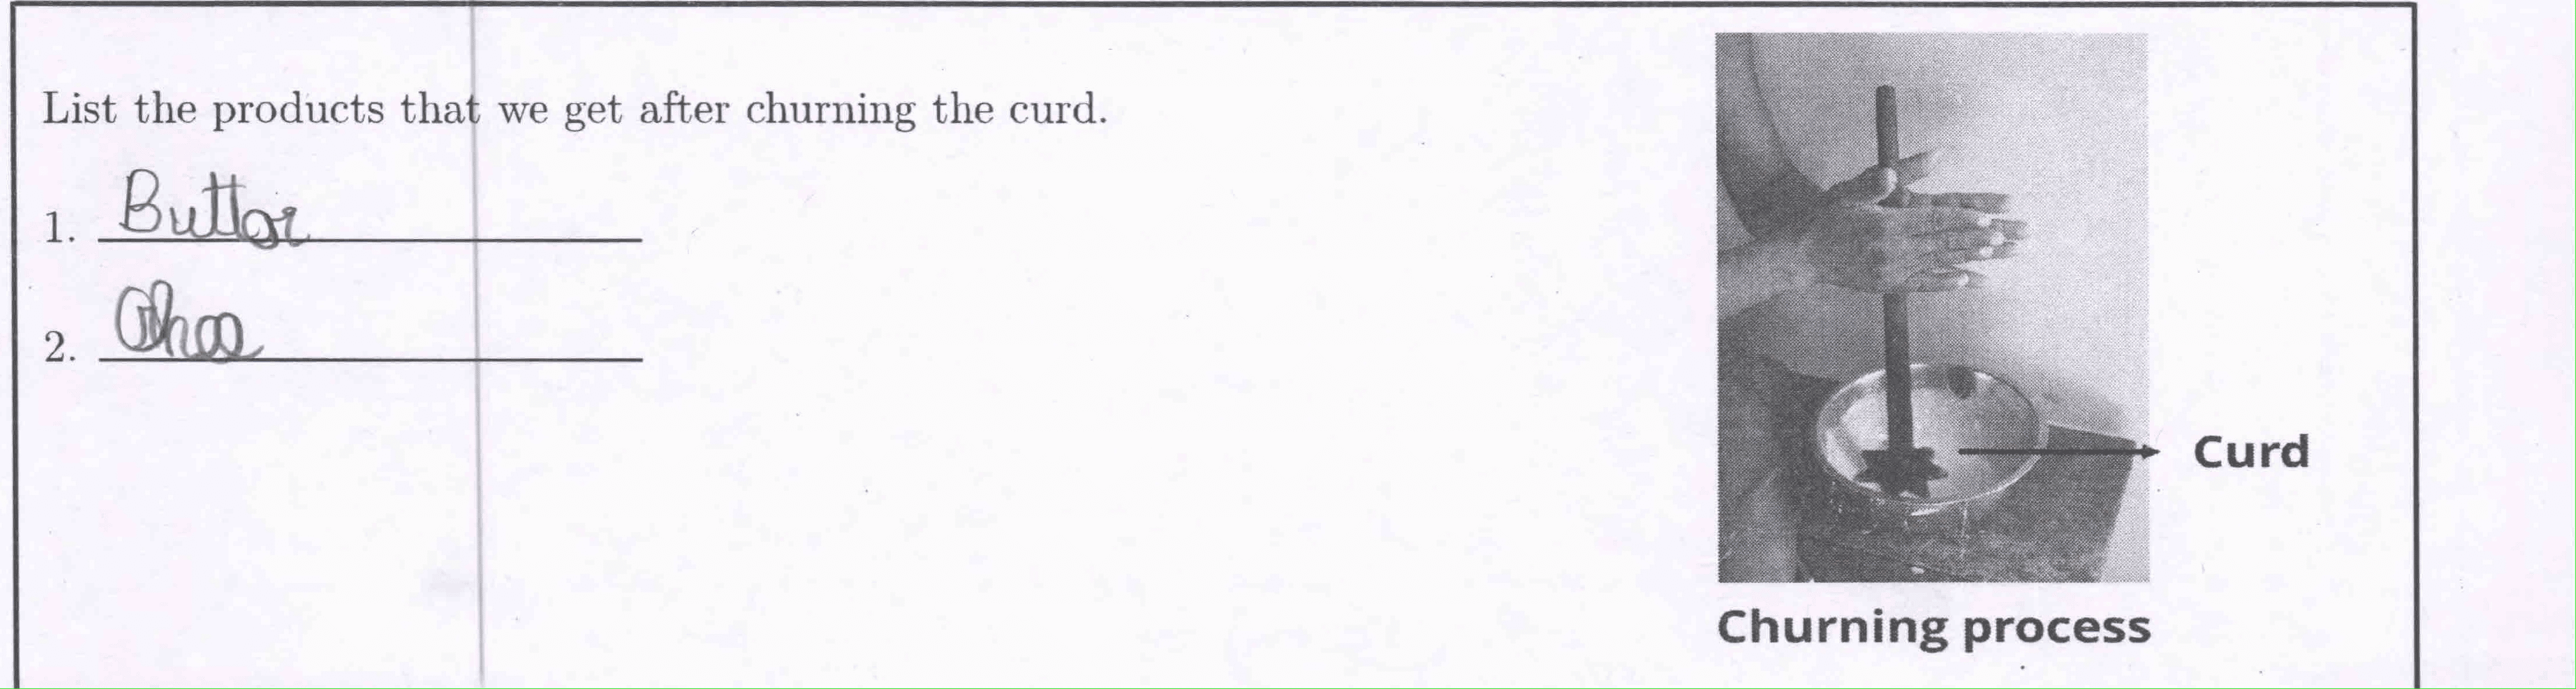
\includegraphics[width=5cm]{Q59_D117140_Science.png}}
    \end{minipage}
    \vspace{10pt}

    % Image: Q59_D117144_Science.png - Scaled height: 5.28mm
    \begin{minipage}{\linewidth}
    \RaggedRight\textbf{\tiny \highred{Varshanth K [C]}} \\ 
    \vspace{4.00pt}\fcolorbox{blue}{white}{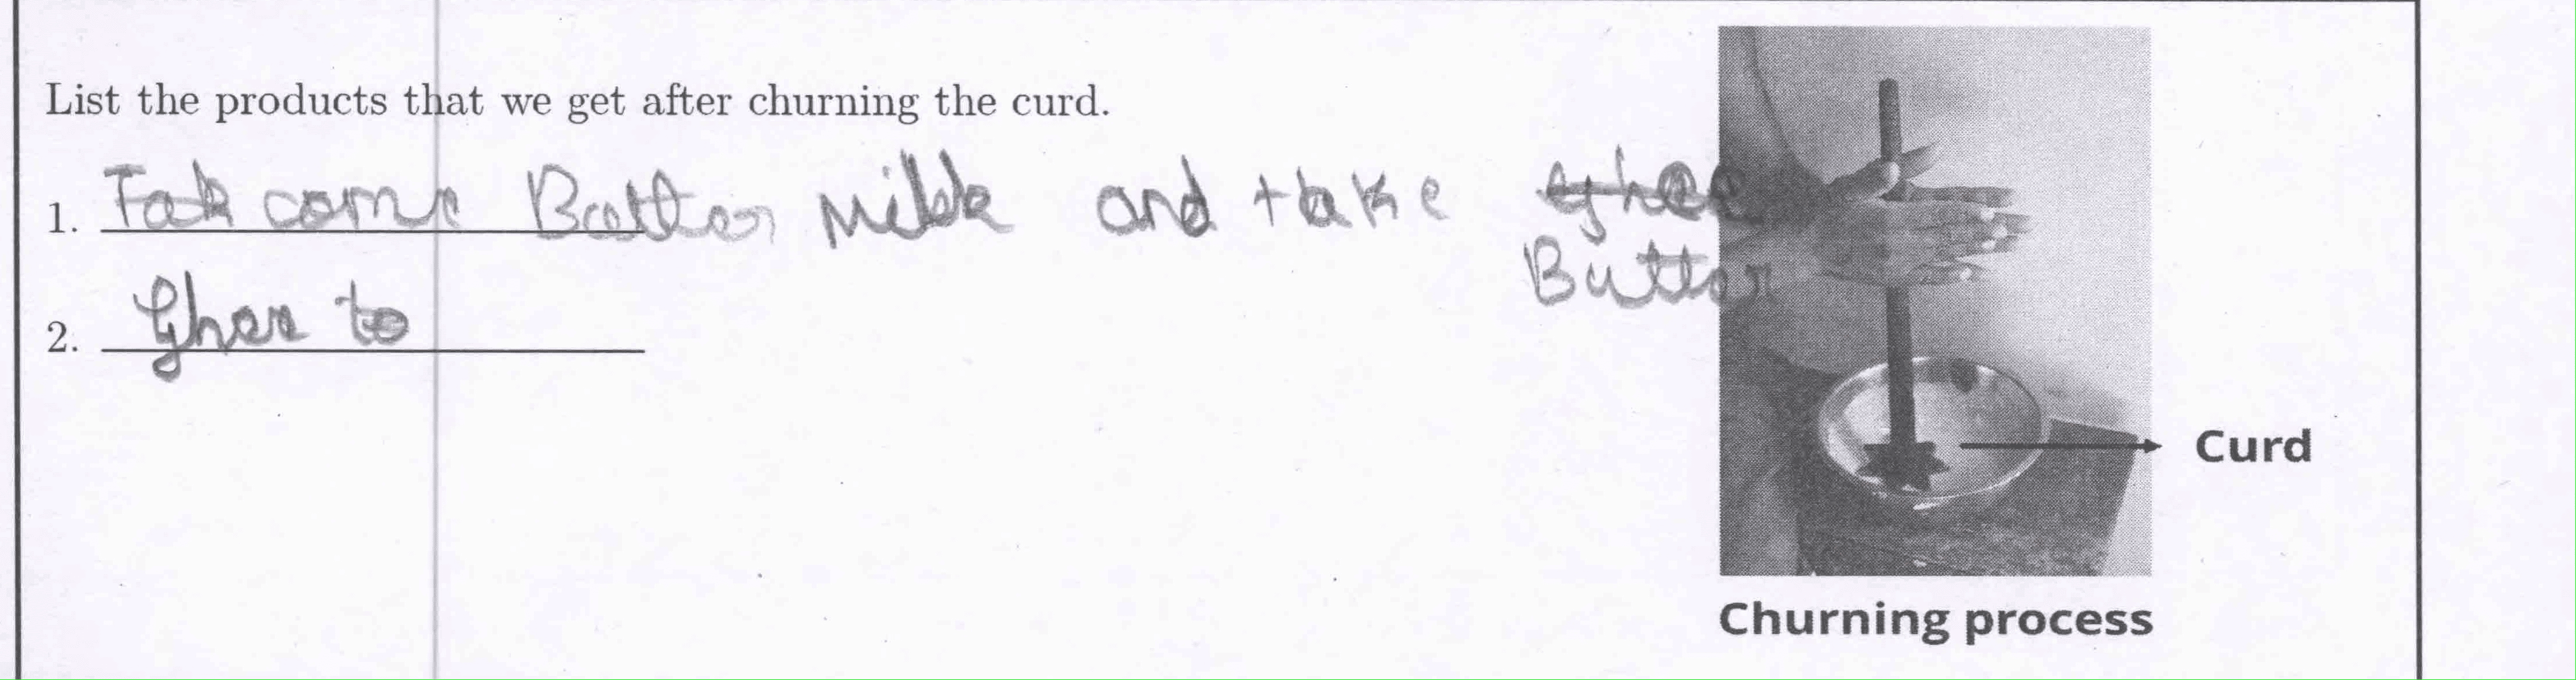
\includegraphics[width=5cm]{Q59_D117144_Science.png}}
    \end{minipage}
    \vspace{10pt}

    % Image: Q59_D117149_Science.png - Scaled height: 4.65mm
    \begin{minipage}{\linewidth}
    \RaggedRight\textbf{\tiny \highgreen{Diya S [B]}} \\ 
    \vspace{4.00pt}\fcolorbox{blue}{white}{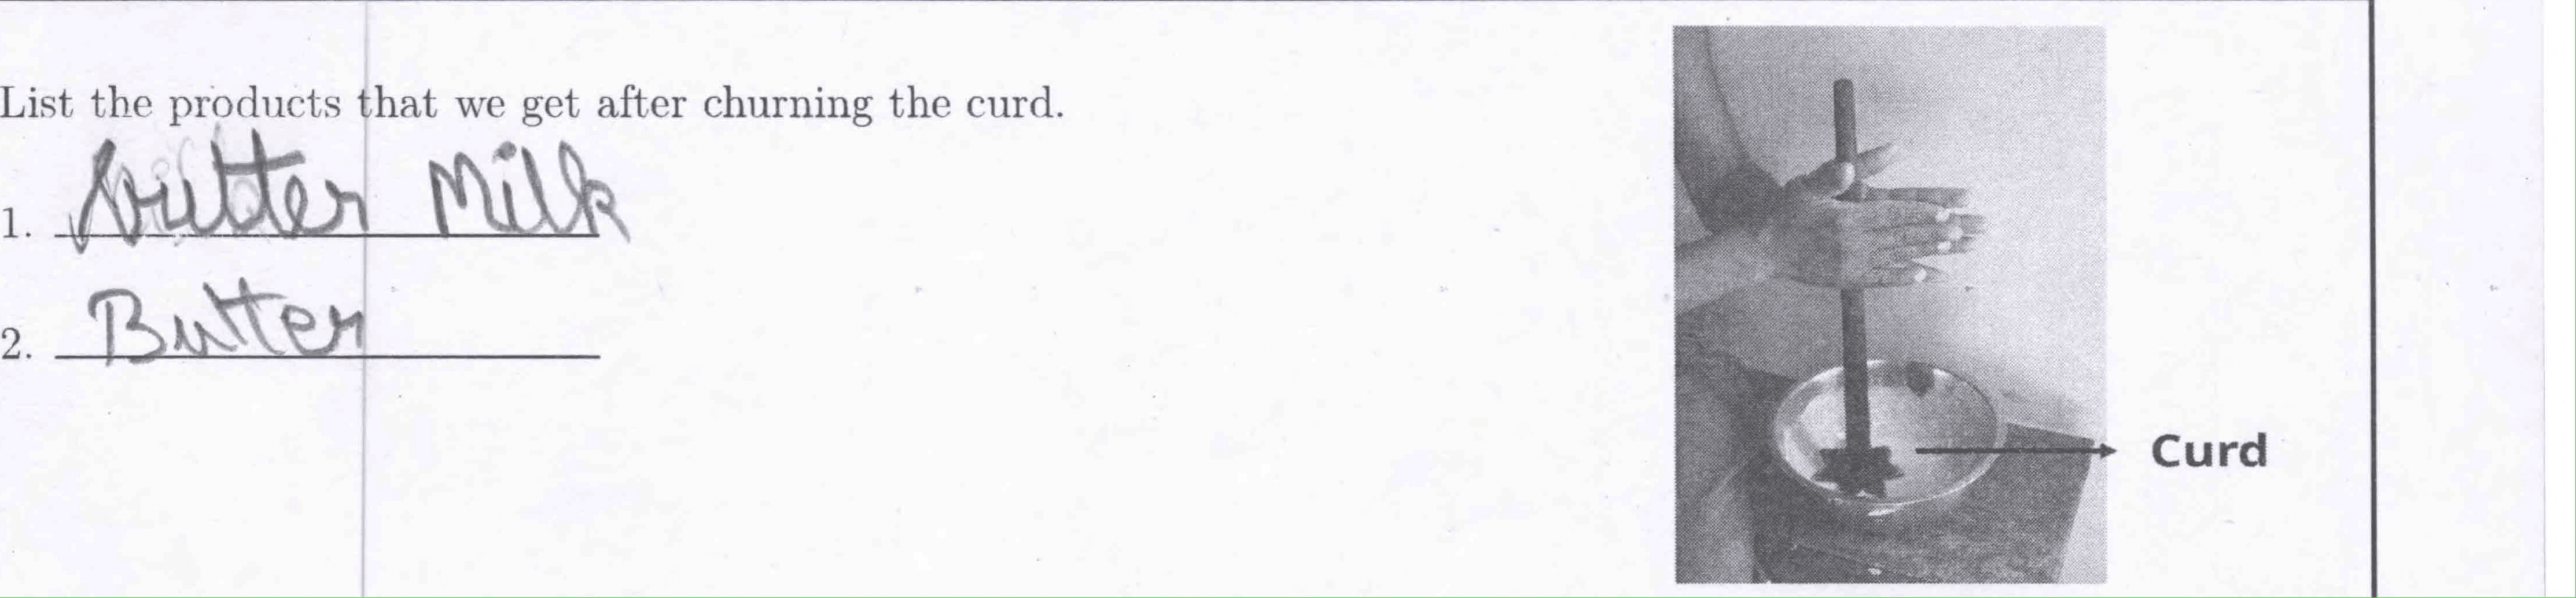
\includegraphics[width=5cm]{Q59_D117149_Science.png}}
    \end{minipage}
    \vspace{10pt}

    % Image: Q59_D117151_Science.png - Scaled height: 5.33mm
    \begin{minipage}{\linewidth}
    \RaggedRight\textbf{\tiny \highred{Karnika R [A]}} \\ 
    \vspace{4.00pt}\fcolorbox{blue}{white}{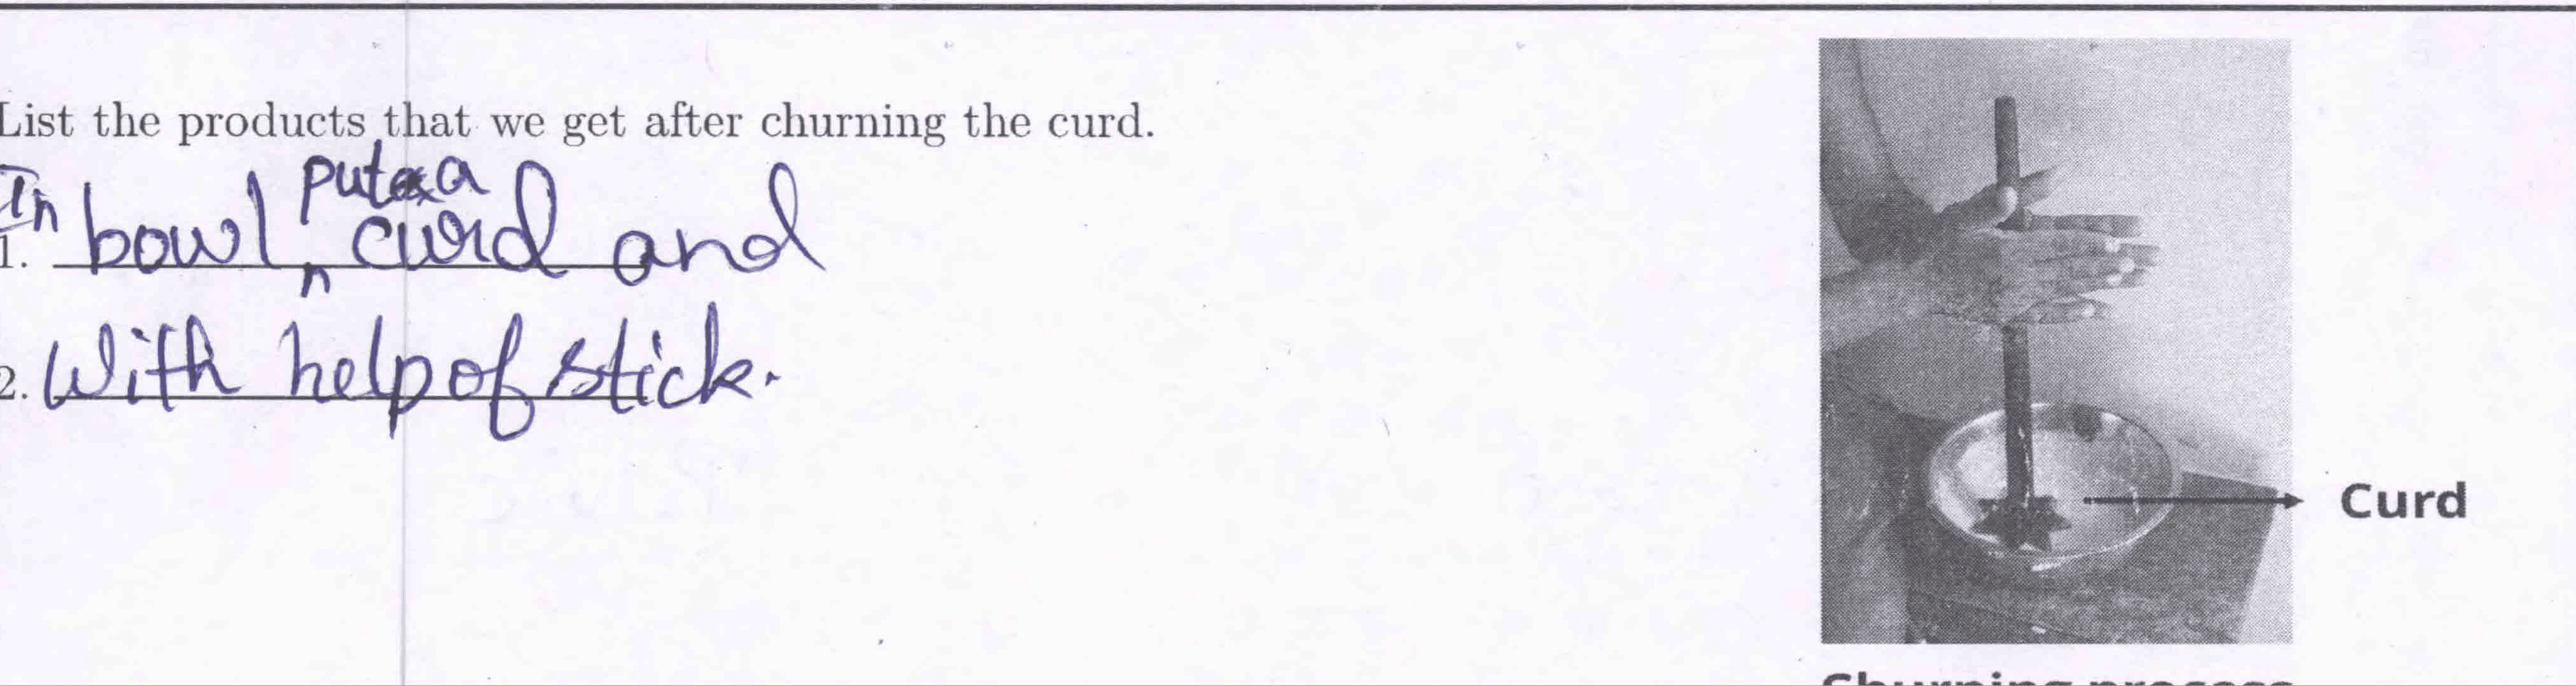
\includegraphics[width=5cm]{Q59_D117151_Science.png}}
    \end{minipage}
    \vspace{10pt}

    % Image: Q59_D117152_Science.png - Scaled height: 5.39mm
    \begin{minipage}{\linewidth}
    \RaggedRight\textbf{\tiny \highgreen{Preethi T [B]}} \\ 
    \vspace{4.00pt}\fcolorbox{blue}{white}{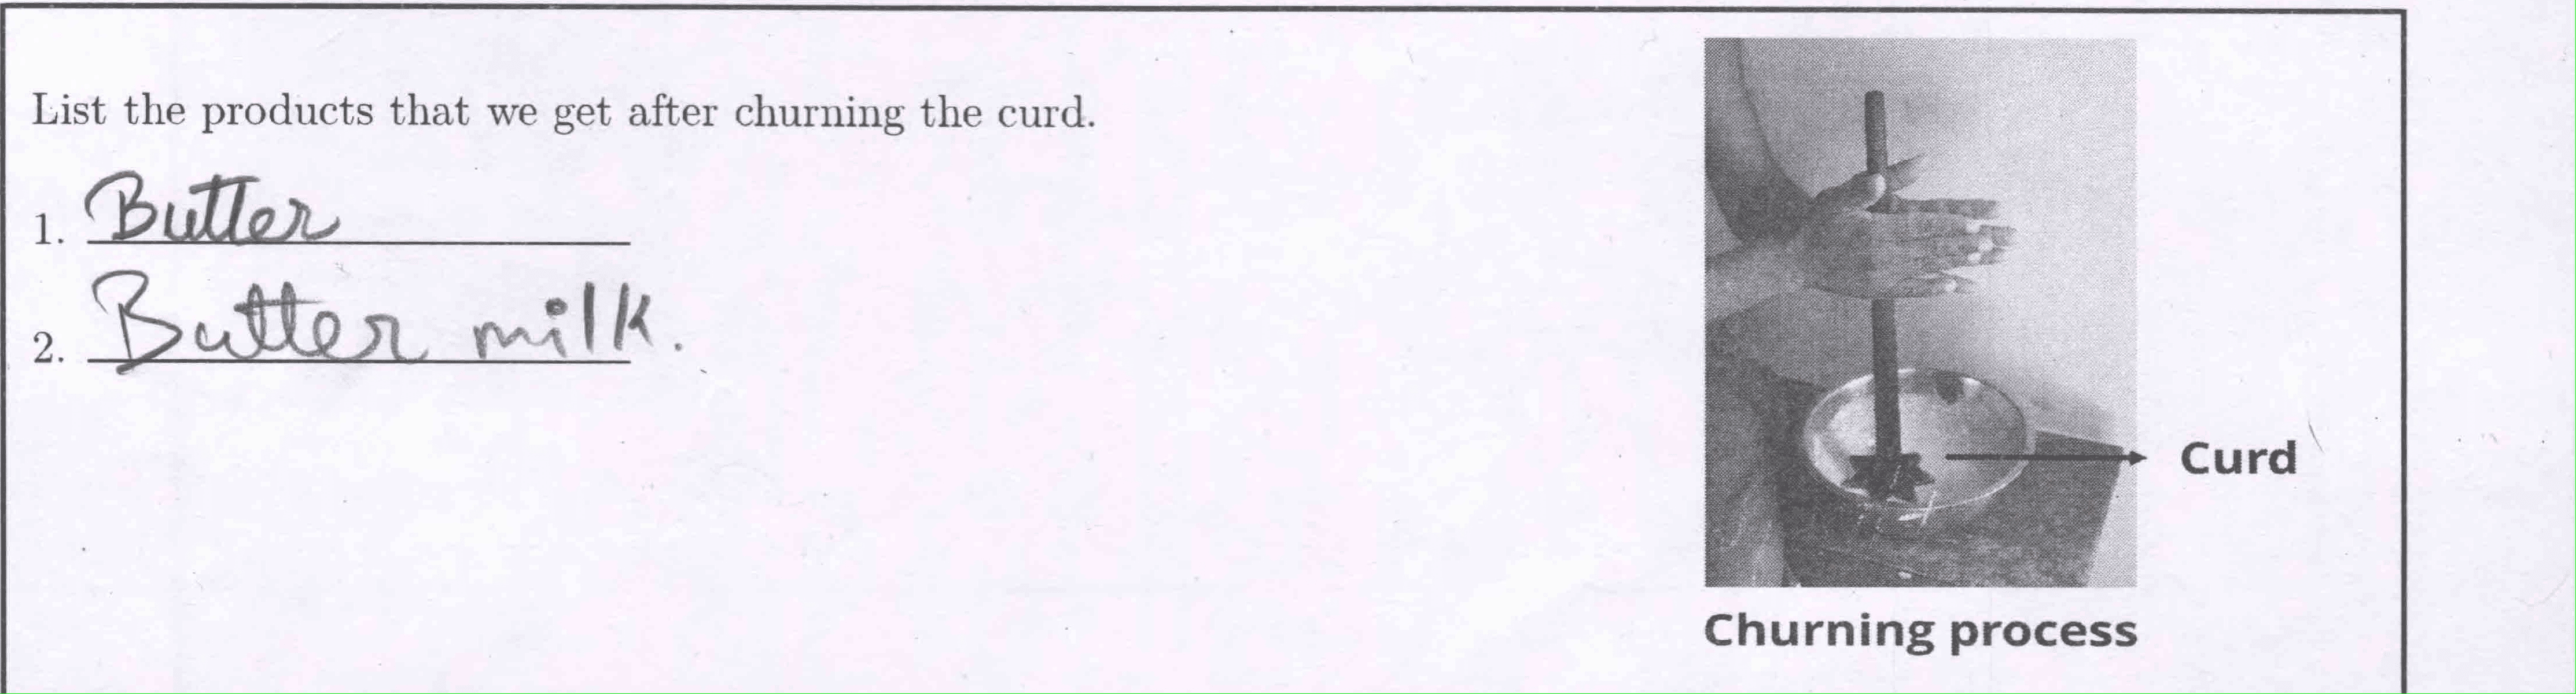
\includegraphics[width=5cm]{Q59_D117152_Science.png}}
    \end{minipage}
    \vspace{10pt}

    % Image: Q59_D117153_Science.png - Scaled height: 4.99mm
    \begin{minipage}{\linewidth}
    \RaggedRight\textbf{\tiny \highgreen{Priyadharshini S A [B]}} \\ 
    \vspace{4.00pt}\fcolorbox{blue}{white}{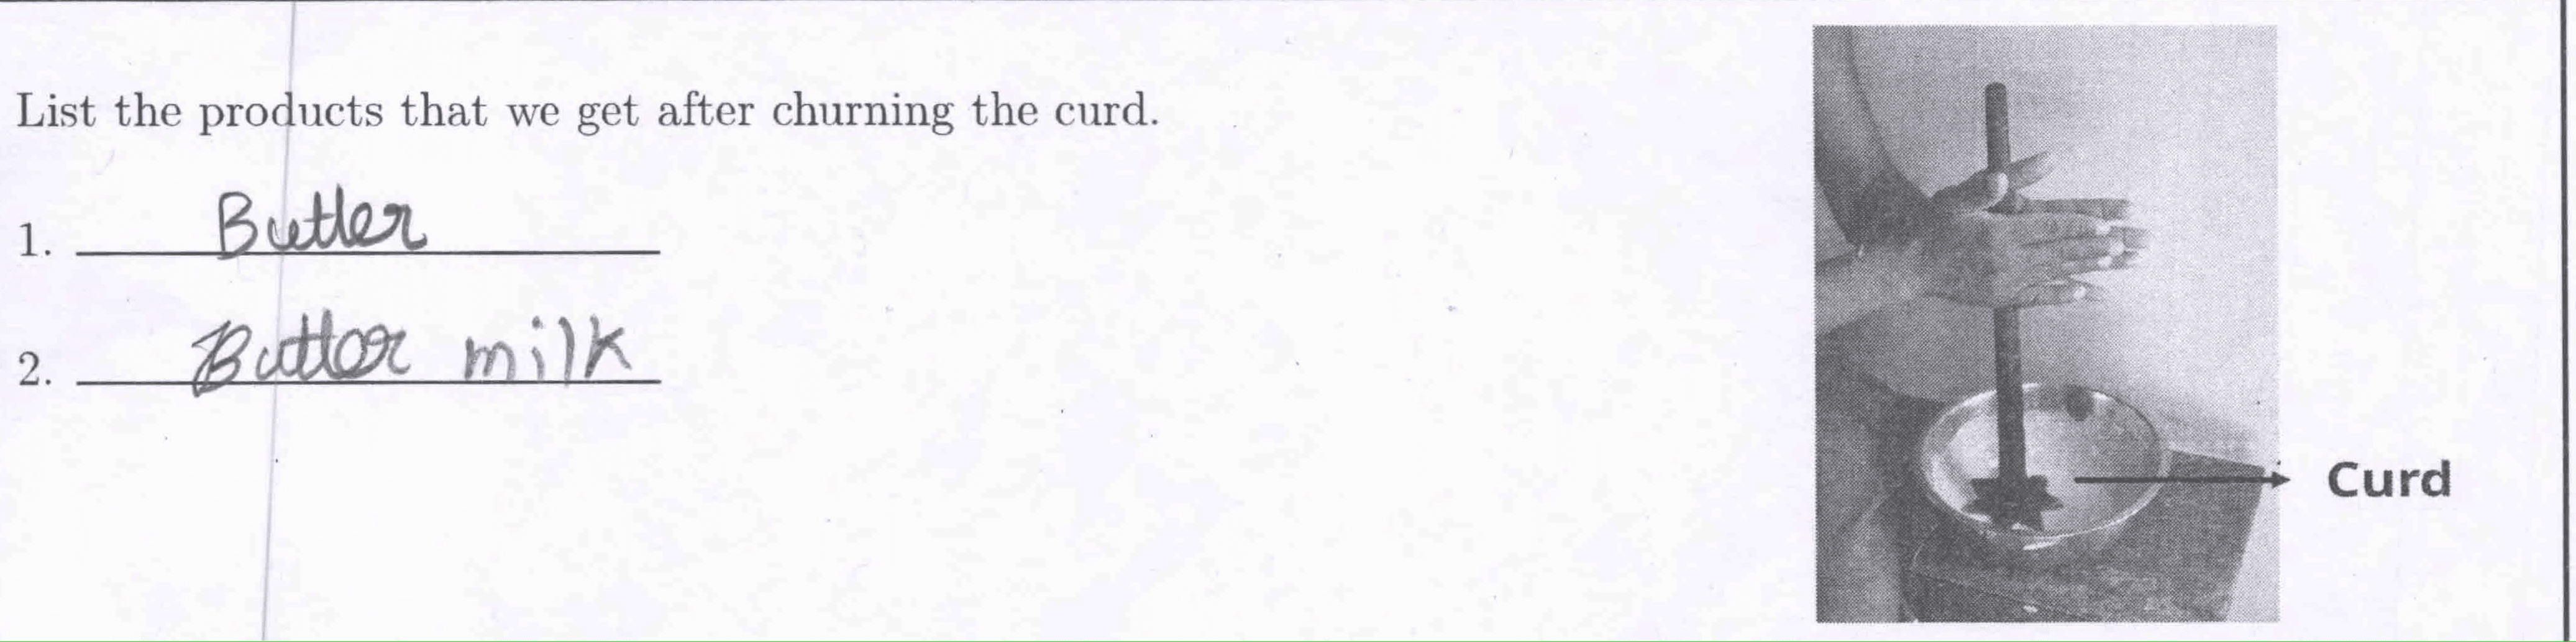
\includegraphics[width=5cm]{Q59_D117153_Science.png}}
    \end{minipage}
    \vspace{10pt}

    \end{multicols}
\end{frame}

\begin{frame}{Q59 - My Answer Responses}
    \vspace{-0.6cm}
    \begin{multicols}{2}

    % Image: Q59_D117156_Science.png - Scaled height: 5.39mm
    \begin{minipage}{\linewidth}
    \RaggedRight\textbf{\tiny \highgreen{Akil E [B]}} \\ 
    \vspace{4.00pt}\fcolorbox{blue}{white}{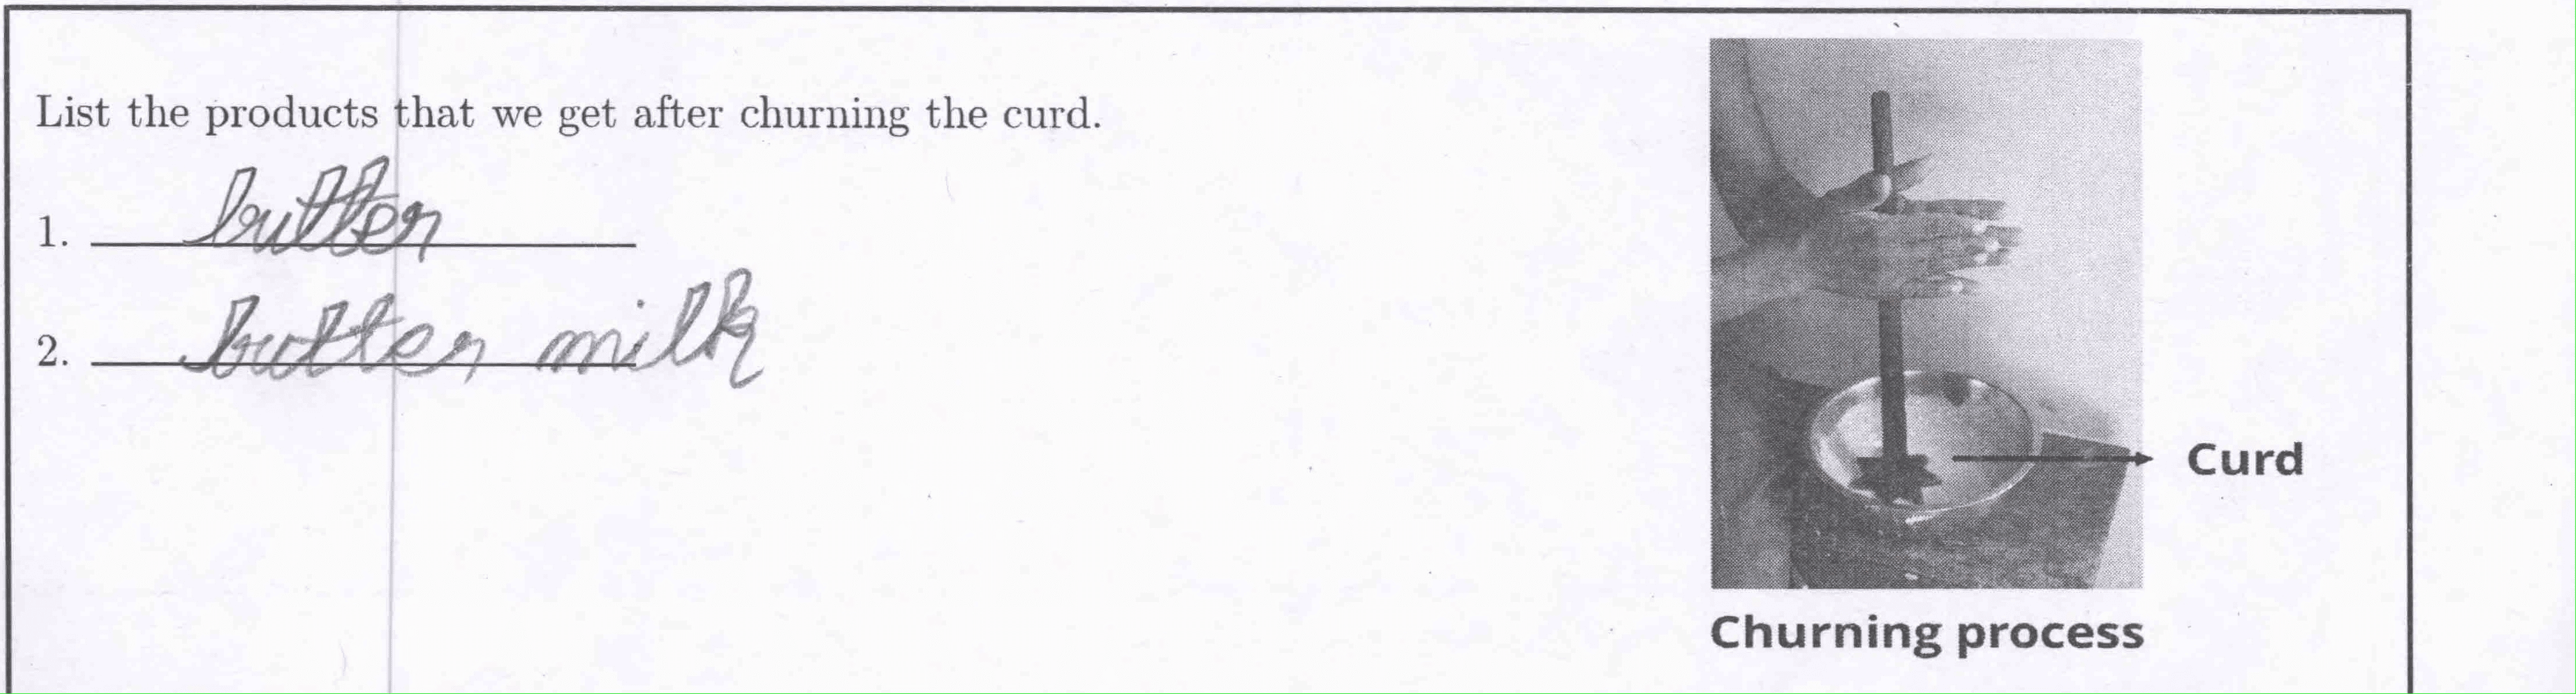
\includegraphics[width=5cm]{Q59_D117156_Science.png}}
    \end{minipage}
    \vspace{10pt}

    % Image: Q59_D117157_Science.png - Scaled height: 4.80mm
    \begin{minipage}{\linewidth}
    \RaggedRight\textbf{\tiny \highred{Aswin P [C]}} \\ 
    \vspace{4.00pt}\fcolorbox{blue}{white}{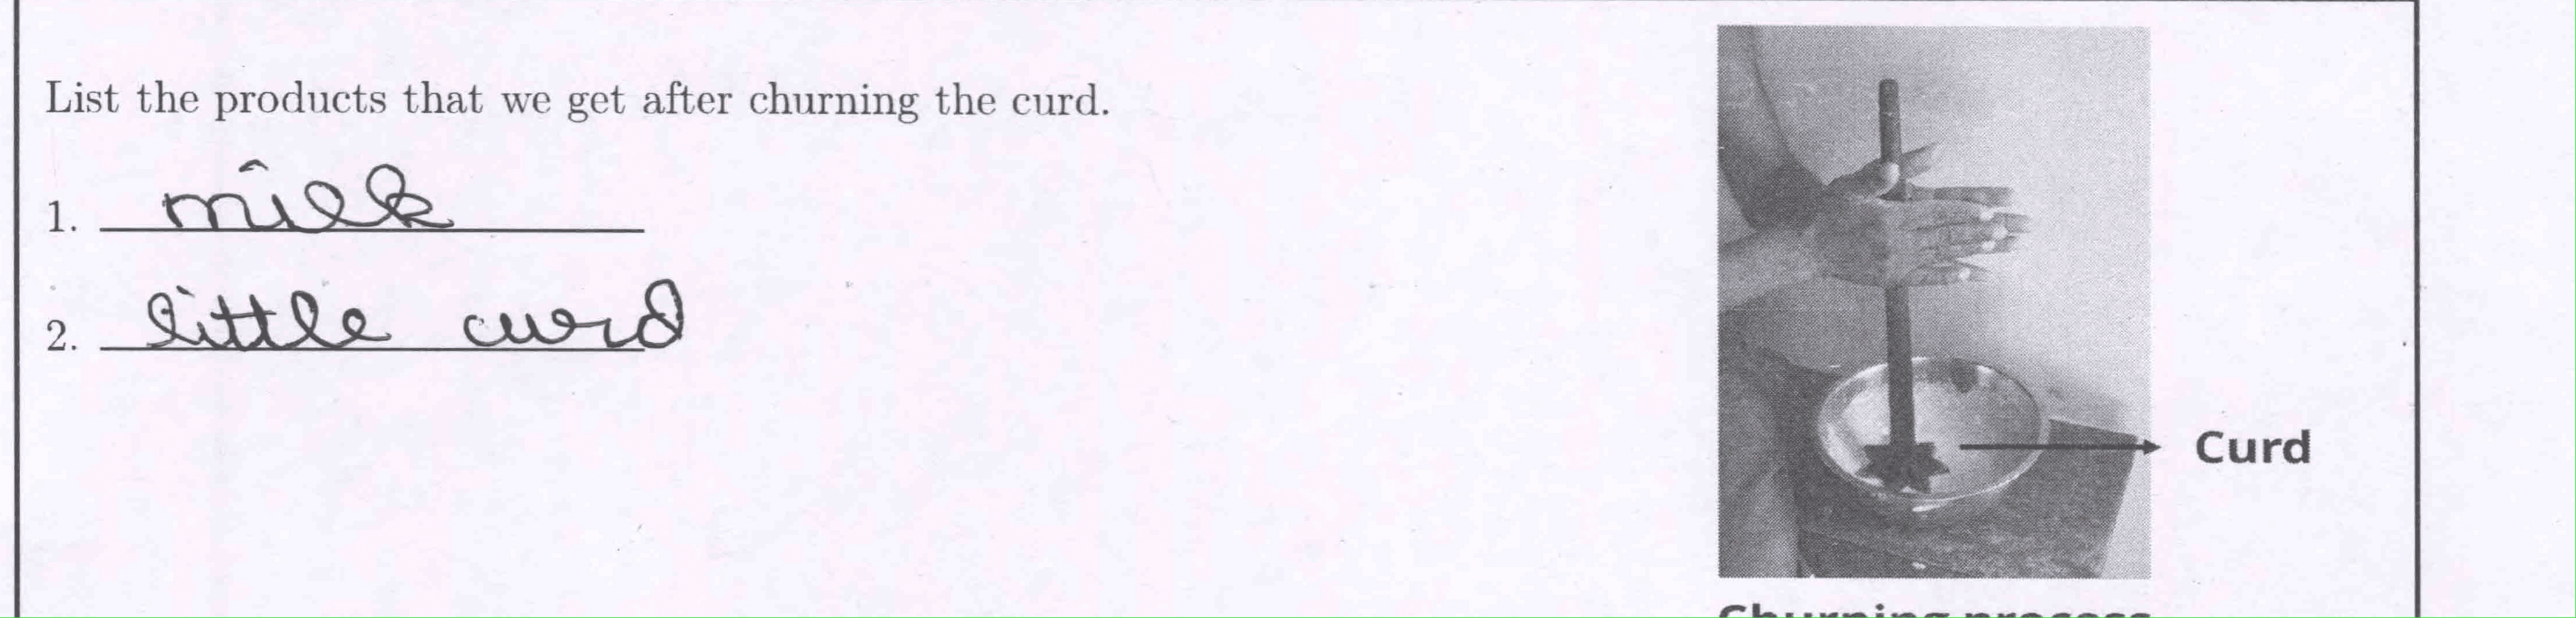
\includegraphics[width=5cm]{Q59_D117157_Science.png}}
    \end{minipage}
    \vspace{10pt}

    % Image: Q59_D117159_Science.png - Scaled height: 5.01mm
    \begin{minipage}{\linewidth}
    \RaggedRight\textbf{\tiny \highred{Gurunathan K R [A]}} \\ 
    \vspace{4.00pt}\fcolorbox{blue}{white}{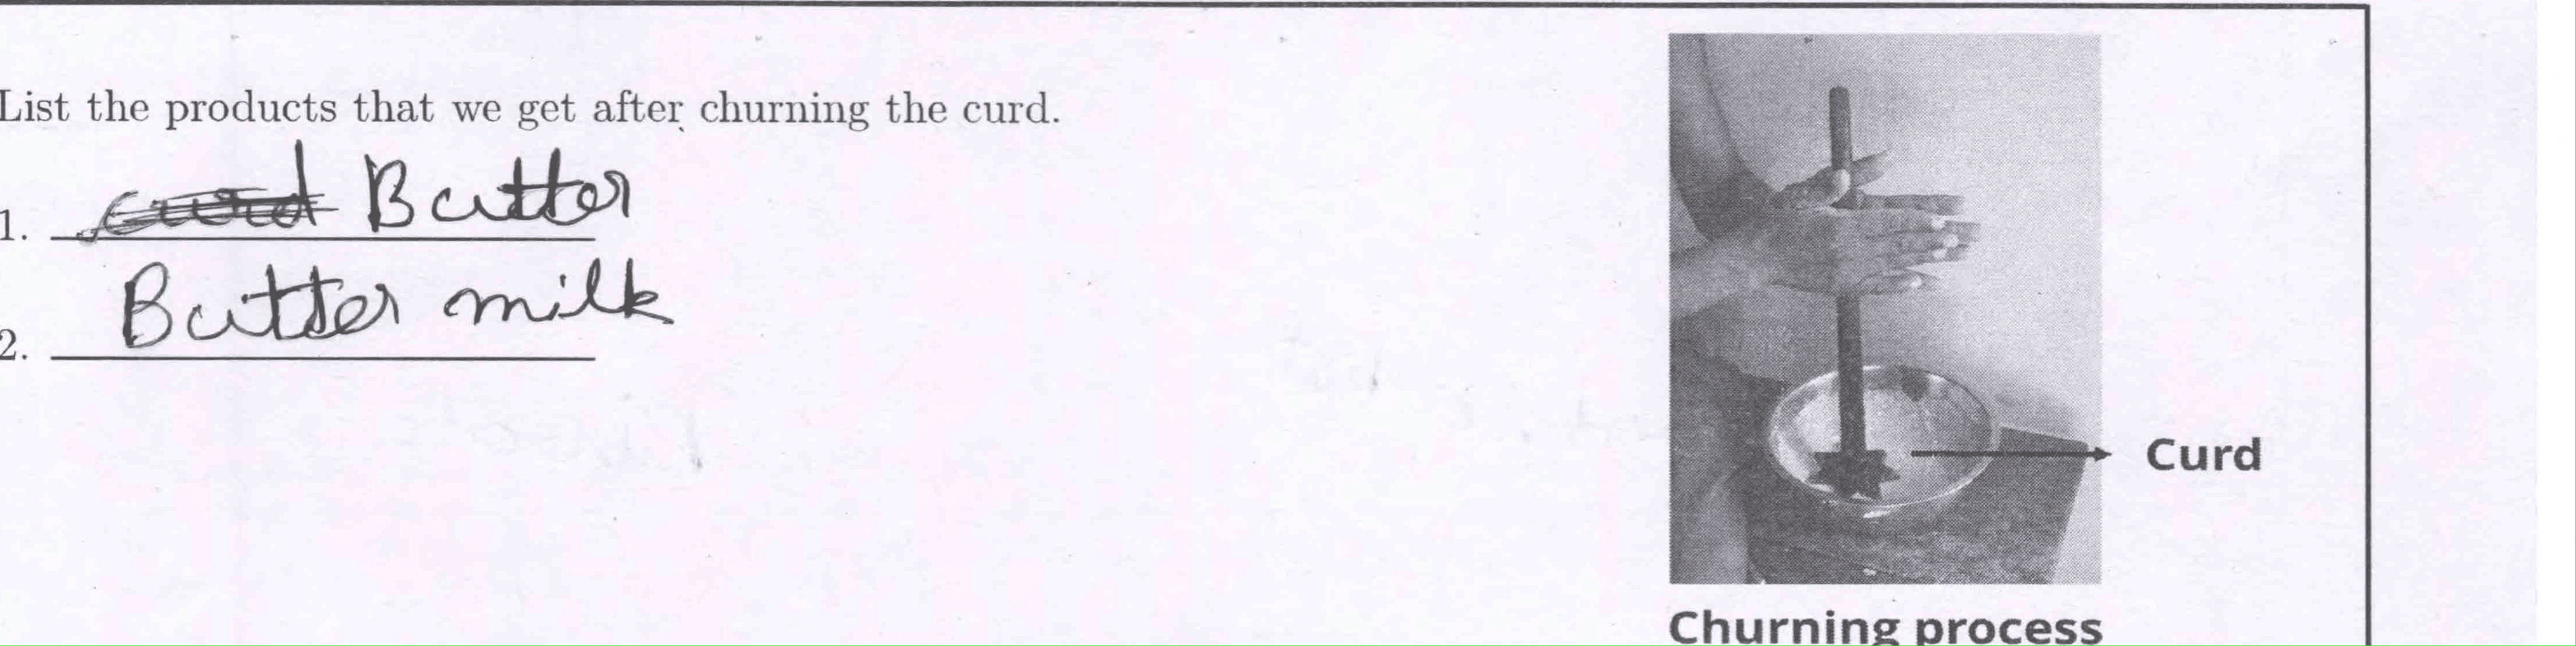
\includegraphics[width=5cm]{Q59_D117159_Science.png}}
    \end{minipage}
    \vspace{10pt}

    % Image: Q59_D117160_Science.png - Scaled height: 5.39mm
    \begin{minipage}{\linewidth}
    \RaggedRight\textbf{\tiny \highgreen{Hrithik T [B]}} \\ 
    \vspace{4.00pt}\fcolorbox{blue}{white}{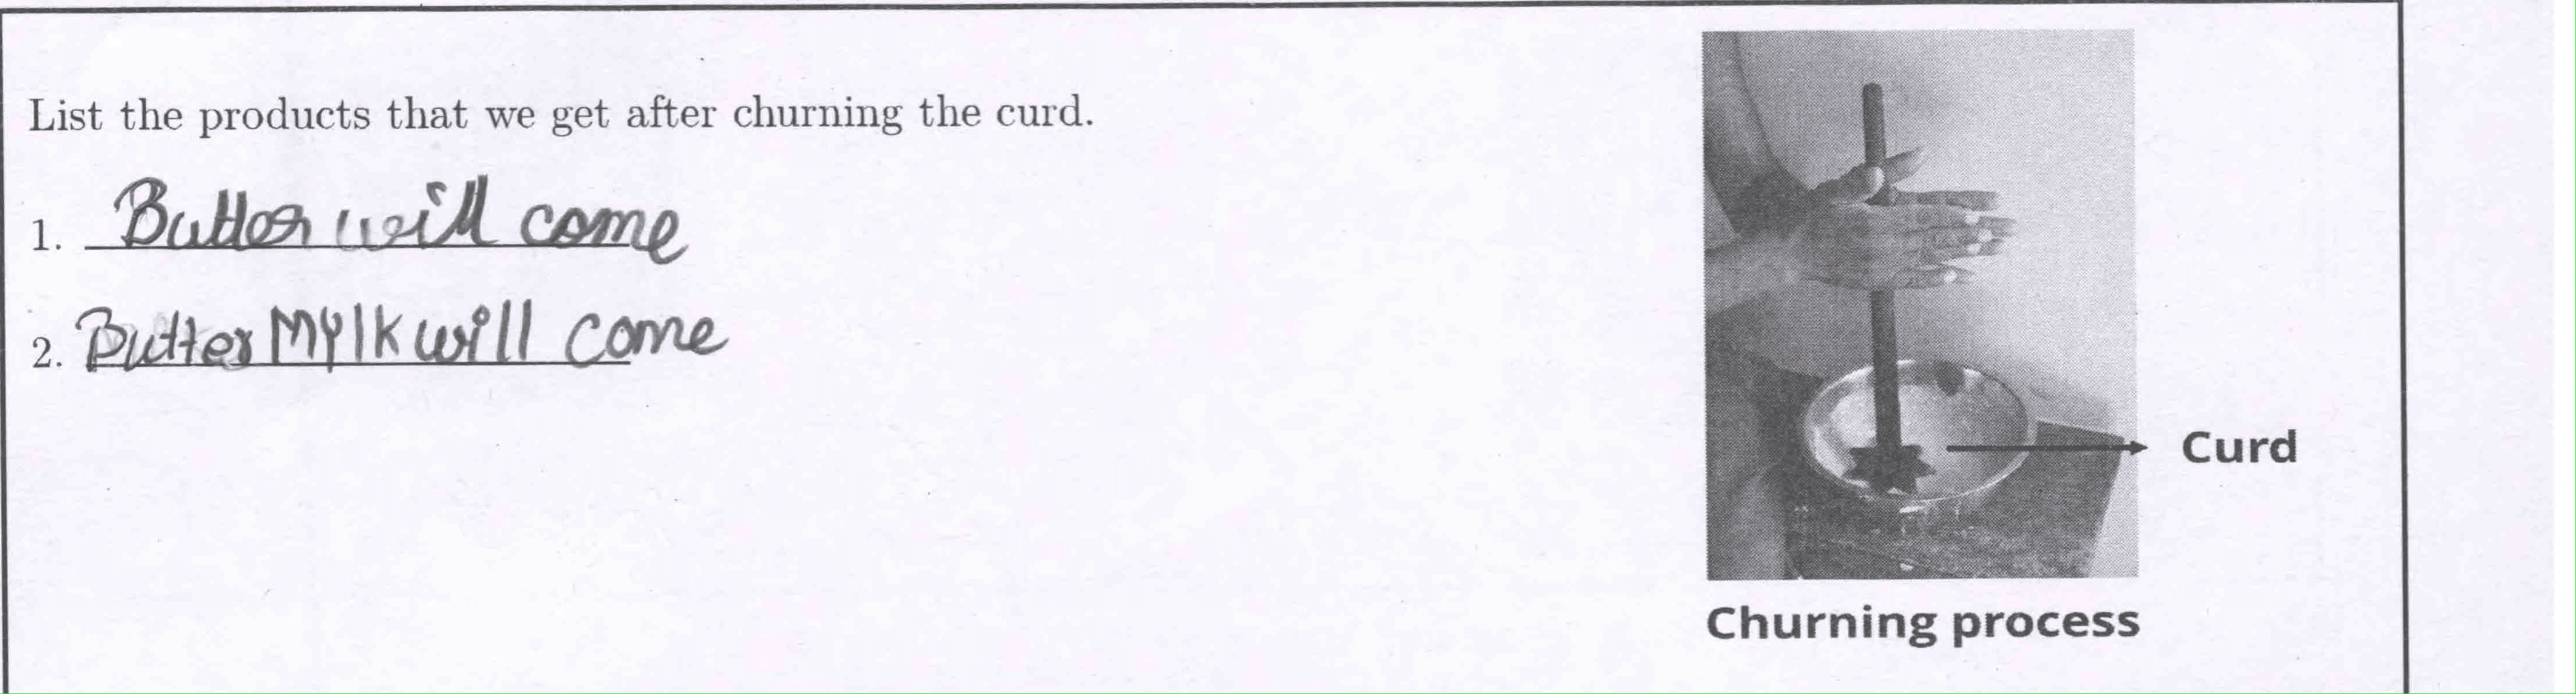
\includegraphics[width=5cm]{Q59_D117160_Science.png}}
    \end{minipage}
    \vspace{10pt}

    % Image: Q59_D117161_Science.png - Scaled height: 4.65mm
    \begin{minipage}{\linewidth}
    \RaggedRight\textbf{\tiny \highgreen{Kiruthik D [B]}} \\ 
    \vspace{4.00pt}\fcolorbox{blue}{white}{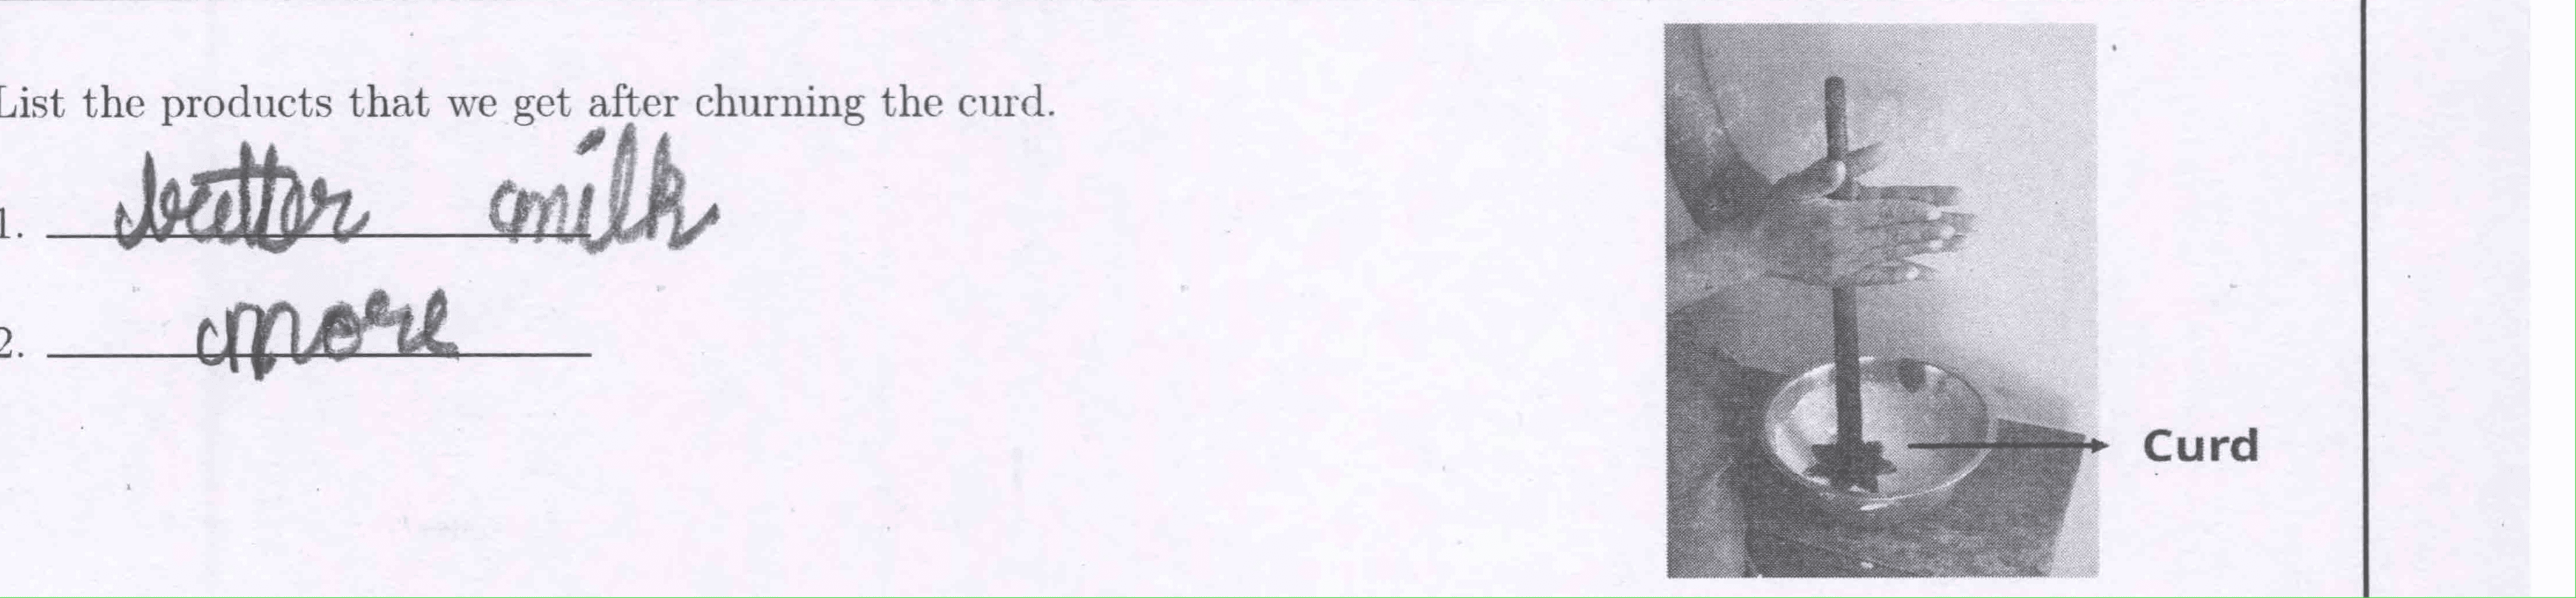
\includegraphics[width=5cm]{Q59_D117161_Science.png}}
    \end{minipage}
    \vspace{10pt}

    % Image: Q59_D117163_Science.png - Scaled height: 4.87mm
    \begin{minipage}{\linewidth}
    \RaggedRight\textbf{\tiny \highred{Manjunath A [C]}} \\ 
    \vspace{4.00pt}\fcolorbox{blue}{white}{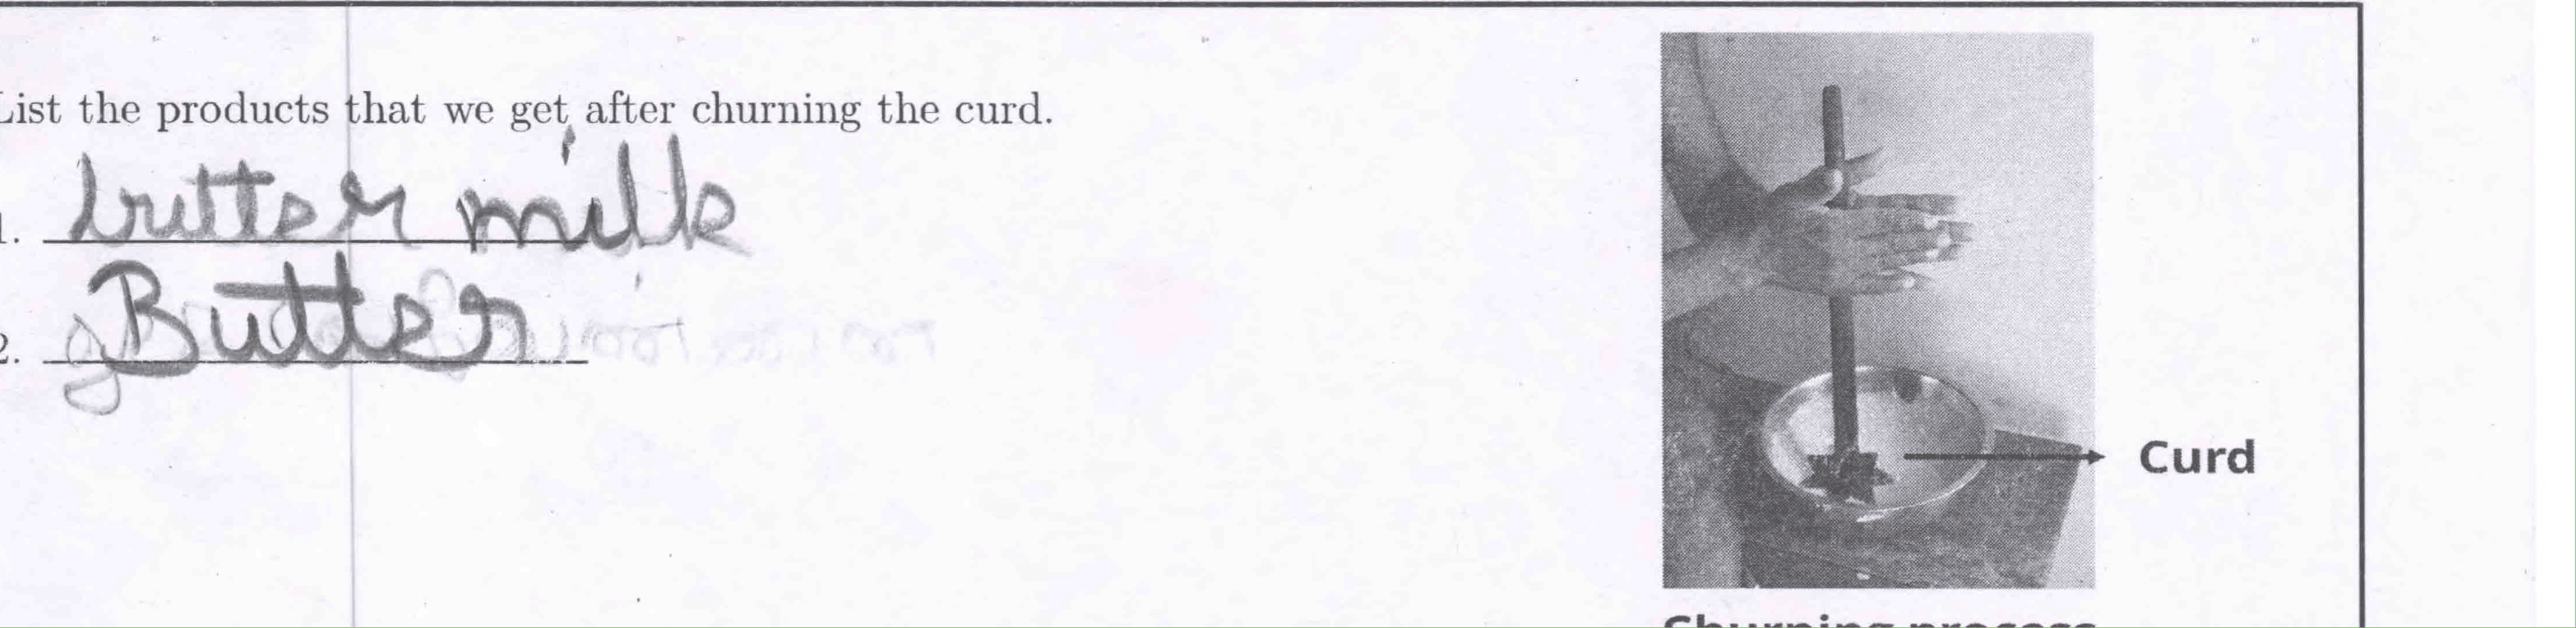
\includegraphics[width=5cm]{Q59_D117163_Science.png}}
    \end{minipage}
    \vspace{10pt}

    % Image: Q59_D117167_Science.png - Scaled height: 4.82mm
    \begin{minipage}{\linewidth}
    \RaggedRight\textbf{\tiny \highgreen{Sriram Karthikeyan V [B]}} \\ 
    \vspace{4.00pt}\fcolorbox{blue}{white}{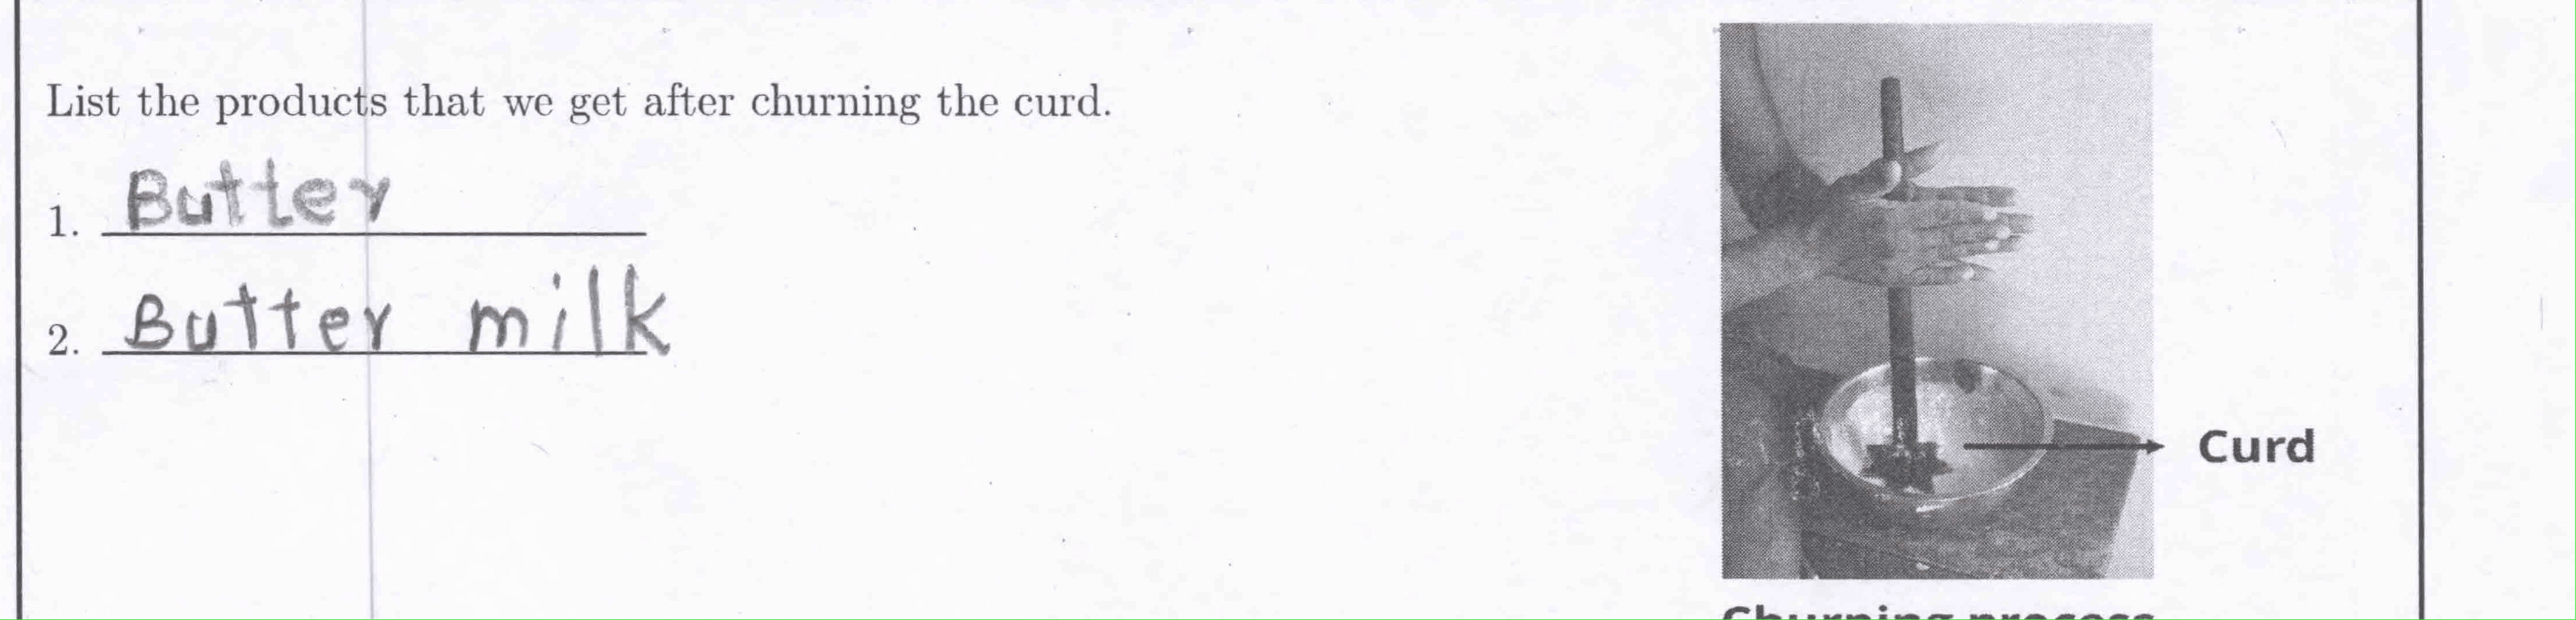
\includegraphics[width=5cm]{Q59_D117167_Science.png}}
    \end{minipage}
    \vspace{10pt}

  

   \end{multicols}
\end{frame}


\begin{frame}[shrink=0.1,label=QPC6QC6S02 - DT - Q17]{Q60 [1. Components of Food]}
\vspace{-0.2cm}


\matextbottomTwoTwo{
myanswerquestion={Write short notes on balanced diet.},
myanswercontent={.},
questionnumber={60}, 
questionTag={C6S02 - DT - Q17},
questiontext={Which of the following food combinations represents the best balanced diet?},
optionA={Fruits and Ice cream},
optionB={Chips and Chicken},
optionC={Chocolate and Ladoo},
optionD={Boiled rice, Vegetables and Curd}, 
correctoption={D},
}


\begin{minipage}{\linewidth}
\hspace{1cm}
\centering
\tiny
\renewcommand{\arraystretch}{1.25}
\begin{tabular}{|M{1.2cm}|M{0.8cm}|M{0.8cm}|M{0.8cm}|M{0.8cm}|M{0.8cm}|}
\hline
Option & A (\ding{55}) & B (\ding{55}) & C (\ding{55}) & \cellcolor{cellgreen} D (\ding{51}) & E \\ 
\hline
6 A & \highno{7\%} & \highno{0\%} & \highno{0\%} & \highno{73\%} & \highno{20\%} \\ 
 \hline 
6 B & \highno{0\%} & \highno{16\%} & \highno{11\%} & \highno{74\%} & \highno{0\%} \\ \hline
\end{tabular}
\end{minipage}

\end{frame}
\begin{frame}{Q60 - My Answer Responses}
    \vspace{-0.6cm}
    \begin{multicols}{2}

    % Image: Q60_D117135_Science.png - Scaled height: 2.26mm
    \begin{minipage}{\linewidth}
    \RaggedRight\textbf{\tiny \highgreen{Dheeresh J A [D]}} \\ 
    \vspace{4.00pt}\fcolorbox{blue}{white}{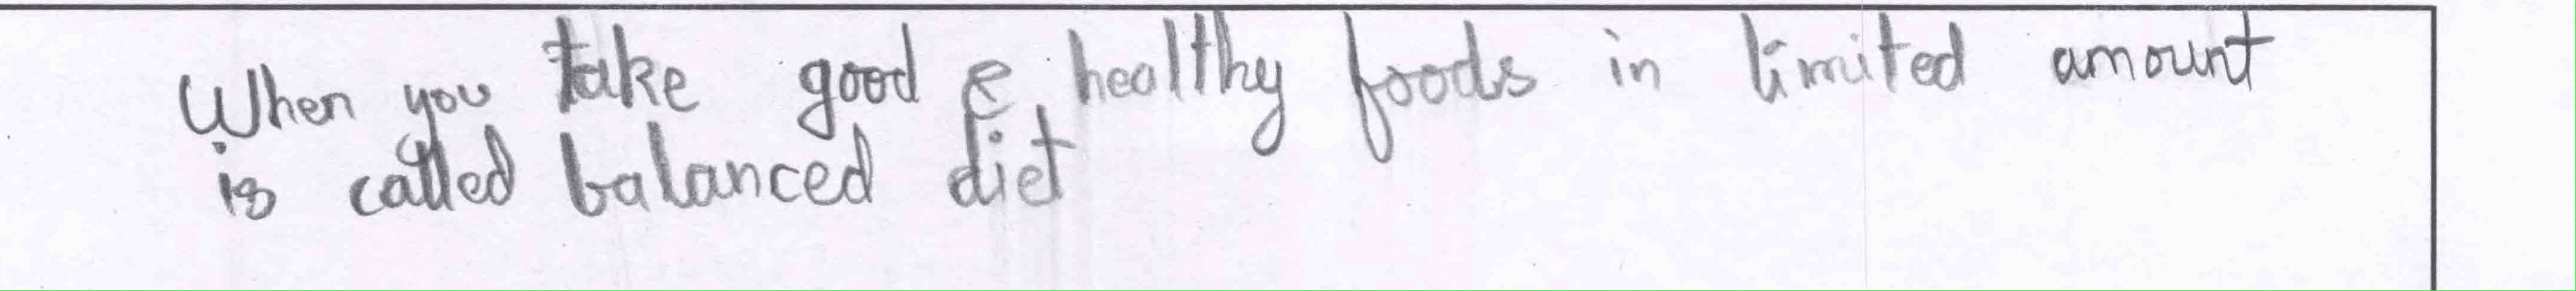
\includegraphics[width=6cm]{Q60_D117135_Science.png}}
    \end{minipage}
    \vspace{10pt}

    % Image: Q60_D117147_Science.png - Scaled height: 2.27mm
    \begin{minipage}{\linewidth}
    \RaggedRight\textbf{\tiny \highgreen{Anusika M [D]}} \\ 
    \vspace{4.00pt}\fcolorbox{blue}{white}{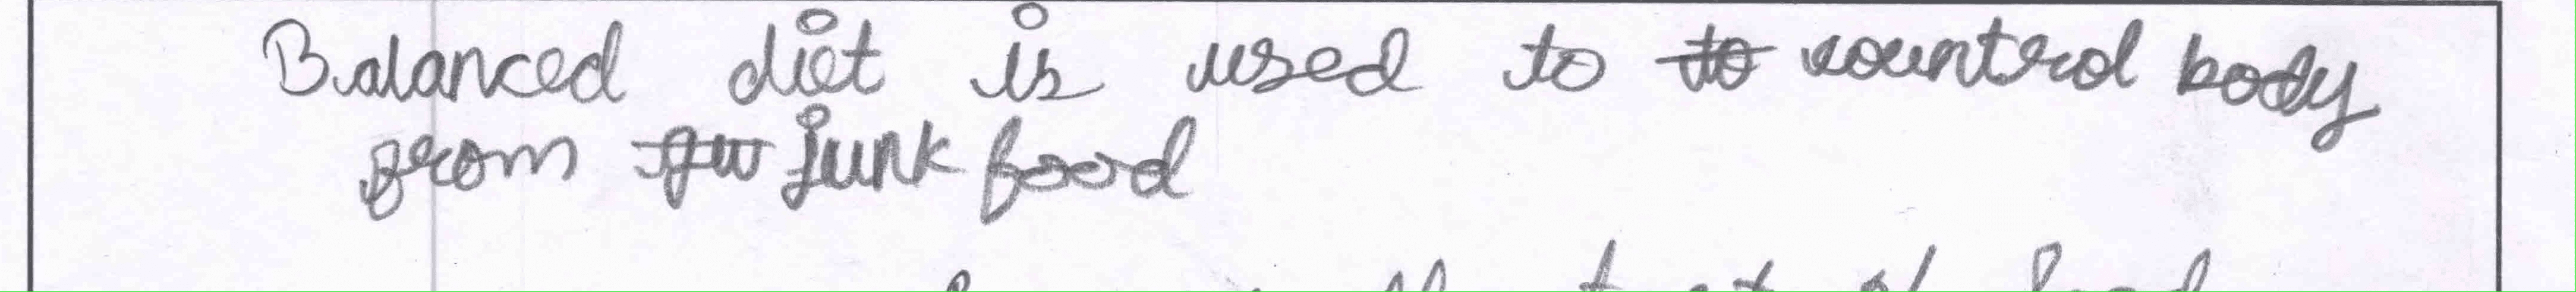
\includegraphics[width=6cm]{Q60_D117147_Science.png}}
    \end{minipage}
    \vspace{10pt}

    % Image: Q60_D117149_Science.png - Scaled height: 3.27mm
    \begin{minipage}{\linewidth}
    \RaggedRight\textbf{\tiny \highgreen{Diya S [D]}} \\ 
    \vspace{4.00pt}\fcolorbox{blue}{white}{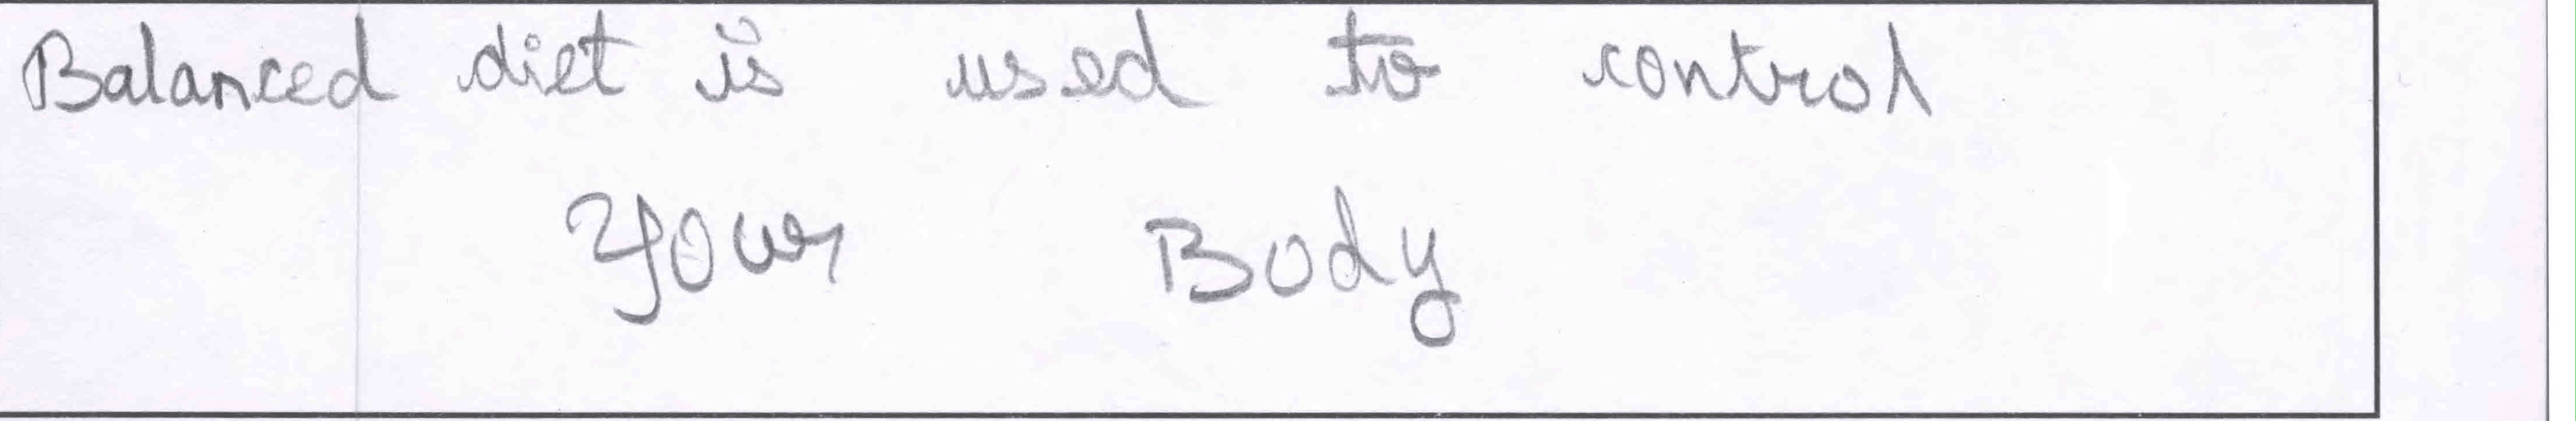
\includegraphics[width=6cm]{Q60_D117149_Science.png}}
    \end{minipage}
    \vspace{10pt}

    % Image: Q60_D117153_Science.png - Scaled height: 3.28mm
    \begin{minipage}{\linewidth}
    \RaggedRight\textbf{\tiny \highgreen{Priyadharshini S A [D]}} \\ 
    \vspace{4.00pt}\fcolorbox{blue}{white}{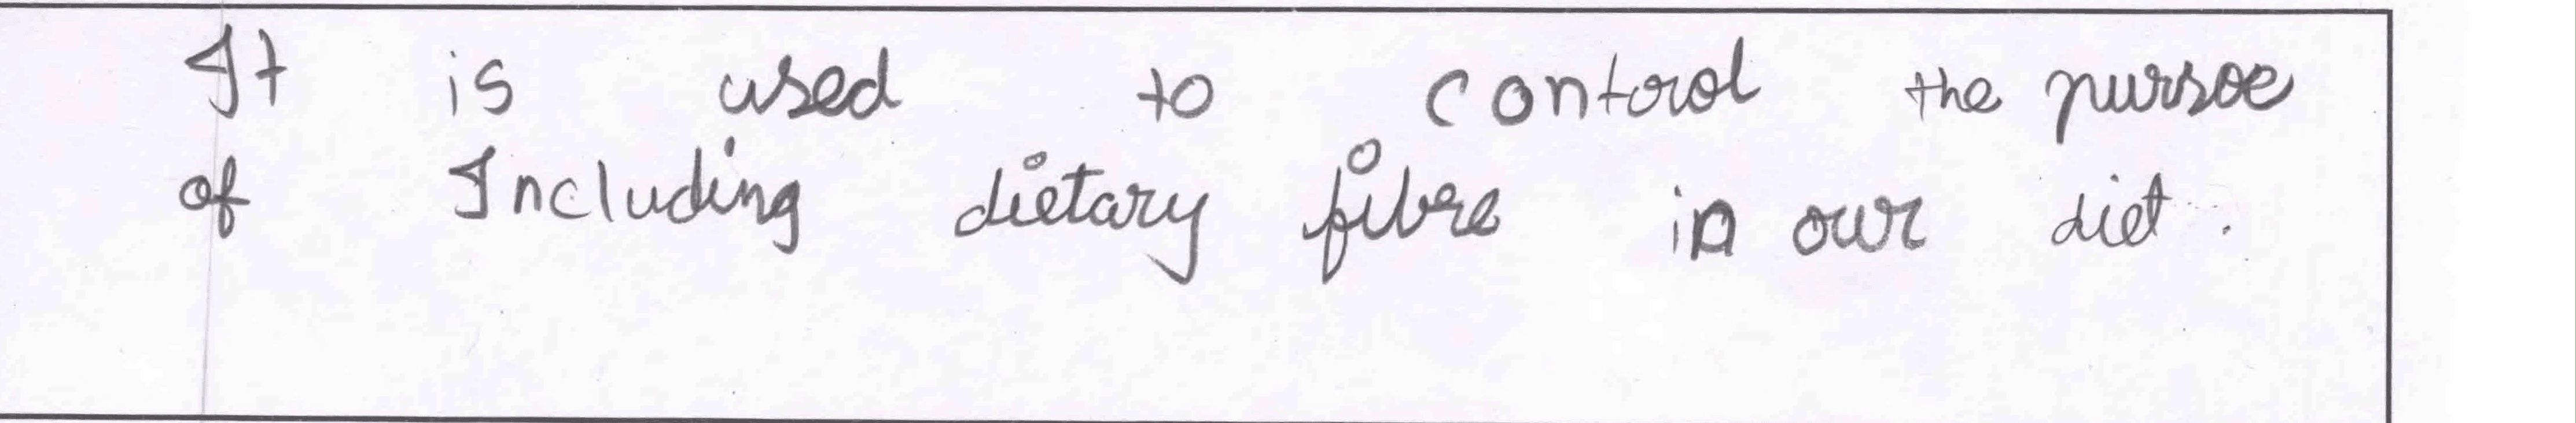
\includegraphics[width=6cm]{Q60_D117153_Science.png}}
    \end{minipage}
    \vspace{10pt}

    % Image: Q60_D117156_Science.png - Scaled height: 3.31mm
    \begin{minipage}{\linewidth}
    \RaggedRight\textbf{\tiny \highgreen{Akil E [D]}} \\ 
    \vspace{4.00pt}\fcolorbox{blue}{white}{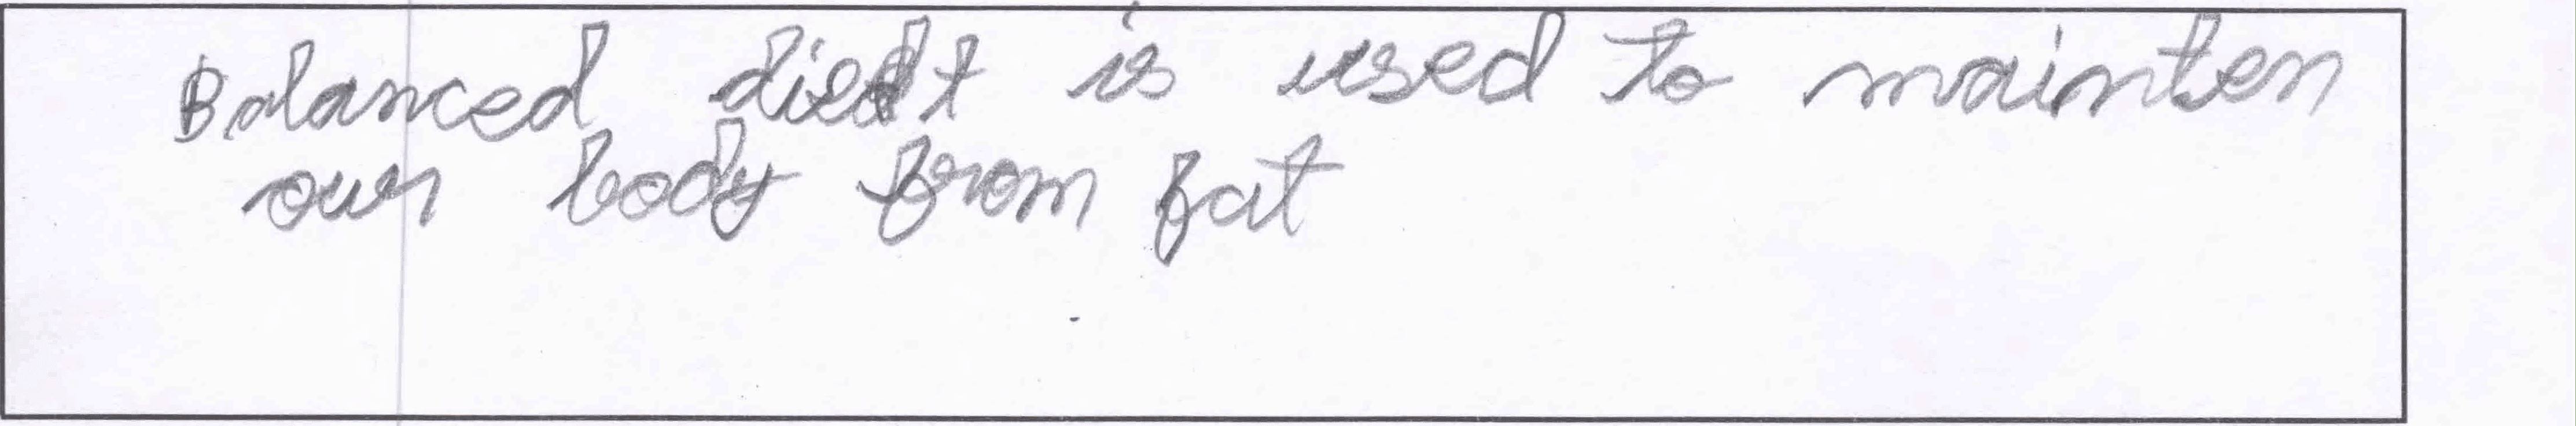
\includegraphics[width=6cm]{Q60_D117156_Science.png}}
    \end{minipage}
    \vspace{10pt}

    % Image: Q60_D117157_Science.png - Scaled height: 3.21mm
    \begin{minipage}{\linewidth}
    \RaggedRight\textbf{\tiny \highgreen{Aswin P [D]}} \\ 
    \vspace{4.00pt}\fcolorbox{blue}{white}{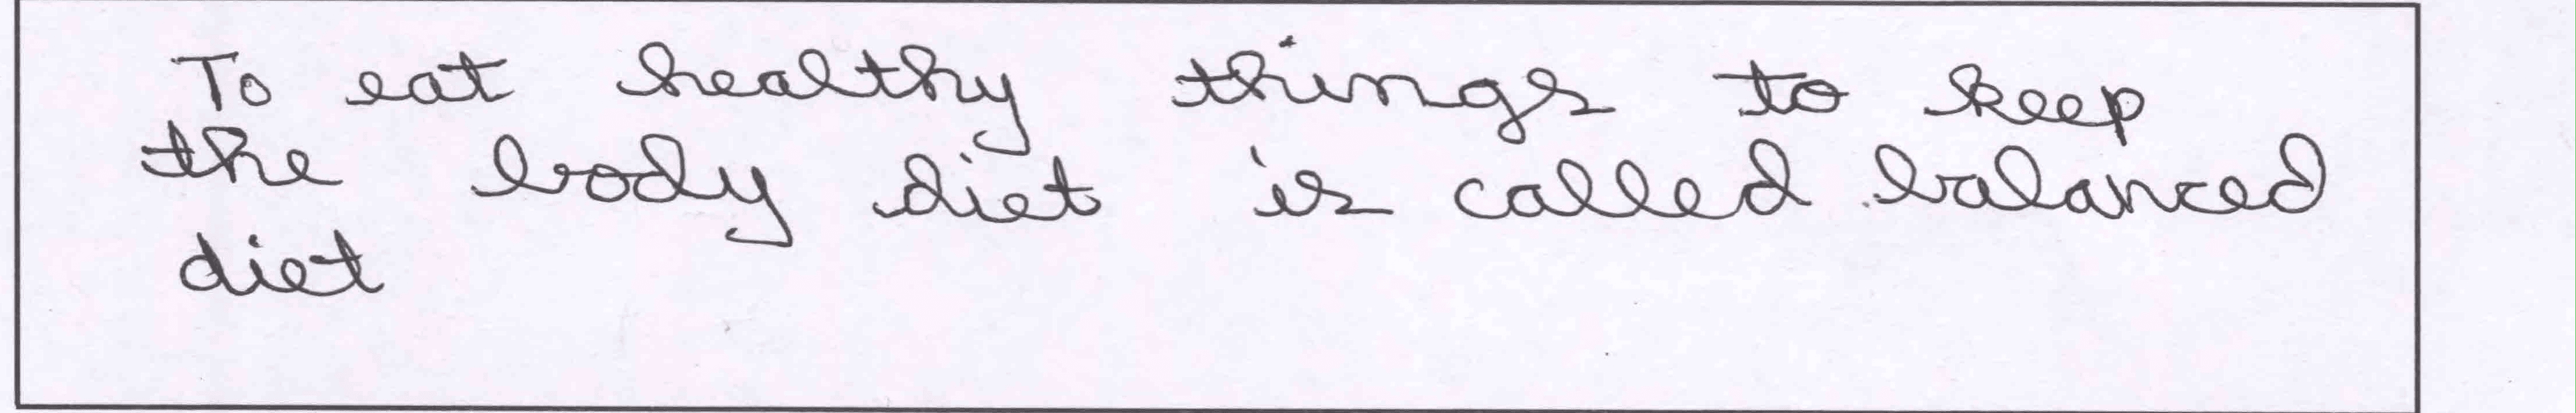
\includegraphics[width=6cm]{Q60_D117157_Science.png}}
    \end{minipage}
    \vspace{10pt}

   

    \end{multicols}
\end{frame}

\begin{frame}{Q60 - My Answer Responses}
    \vspace{-0.6cm}
    \begin{multicols}{2}
 % Image: Q60_D117161_Science.png - Scaled height: 3.23mm
    \begin{minipage}{\linewidth}
    \RaggedRight\textbf{\tiny \highgreen{Kiruthik D [D]}} \\ 
    \vspace{4.00pt}\fcolorbox{blue}{white}{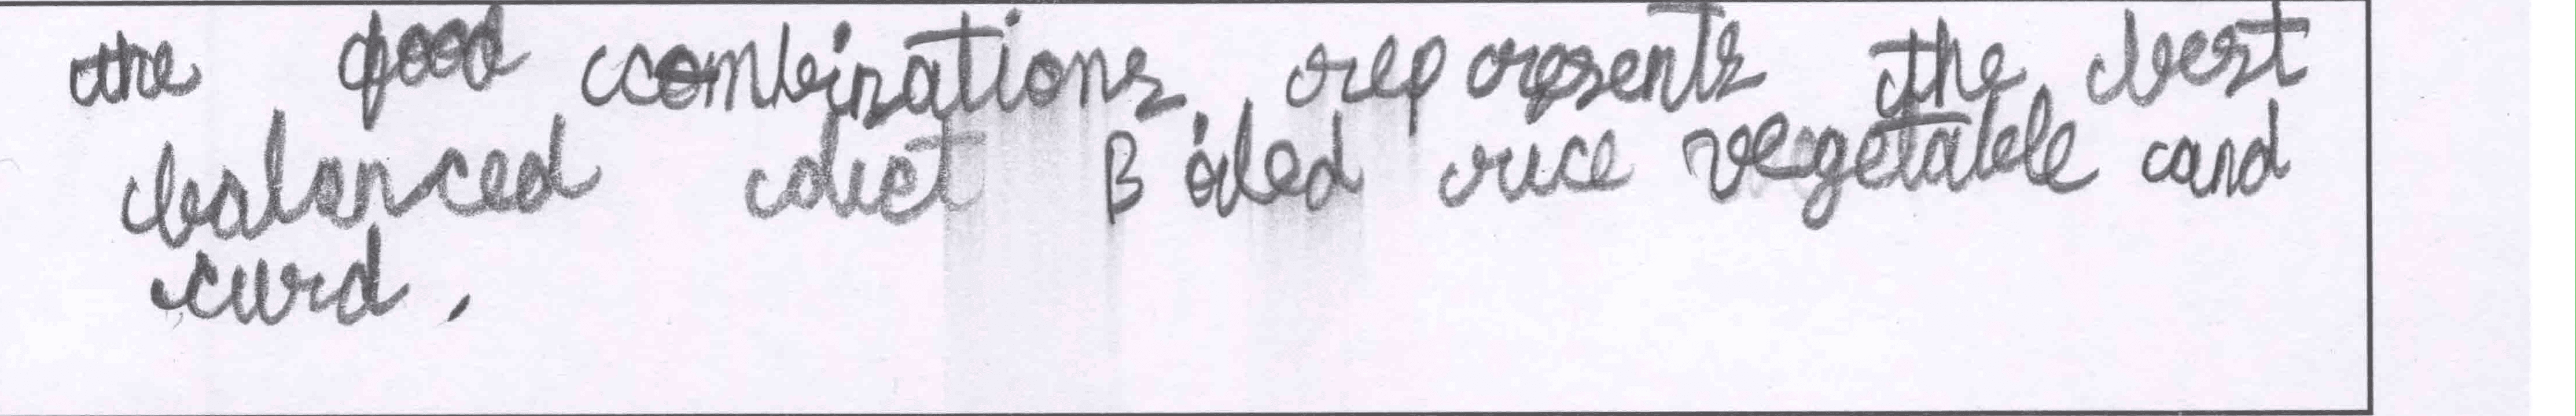
\includegraphics[width=6cm]{Q60_D117161_Science.png}}
    \end{minipage}
    \vspace{10pt}

    % Image: Q60_D117170_Science.png - Scaled height: 3.29mm
    \begin{minipage}{\linewidth}
    \RaggedRight\textbf{\tiny \highgreen{Cemmozhi S [D]}} \\ 
    \vspace{4.00pt}\fcolorbox{blue}{white}{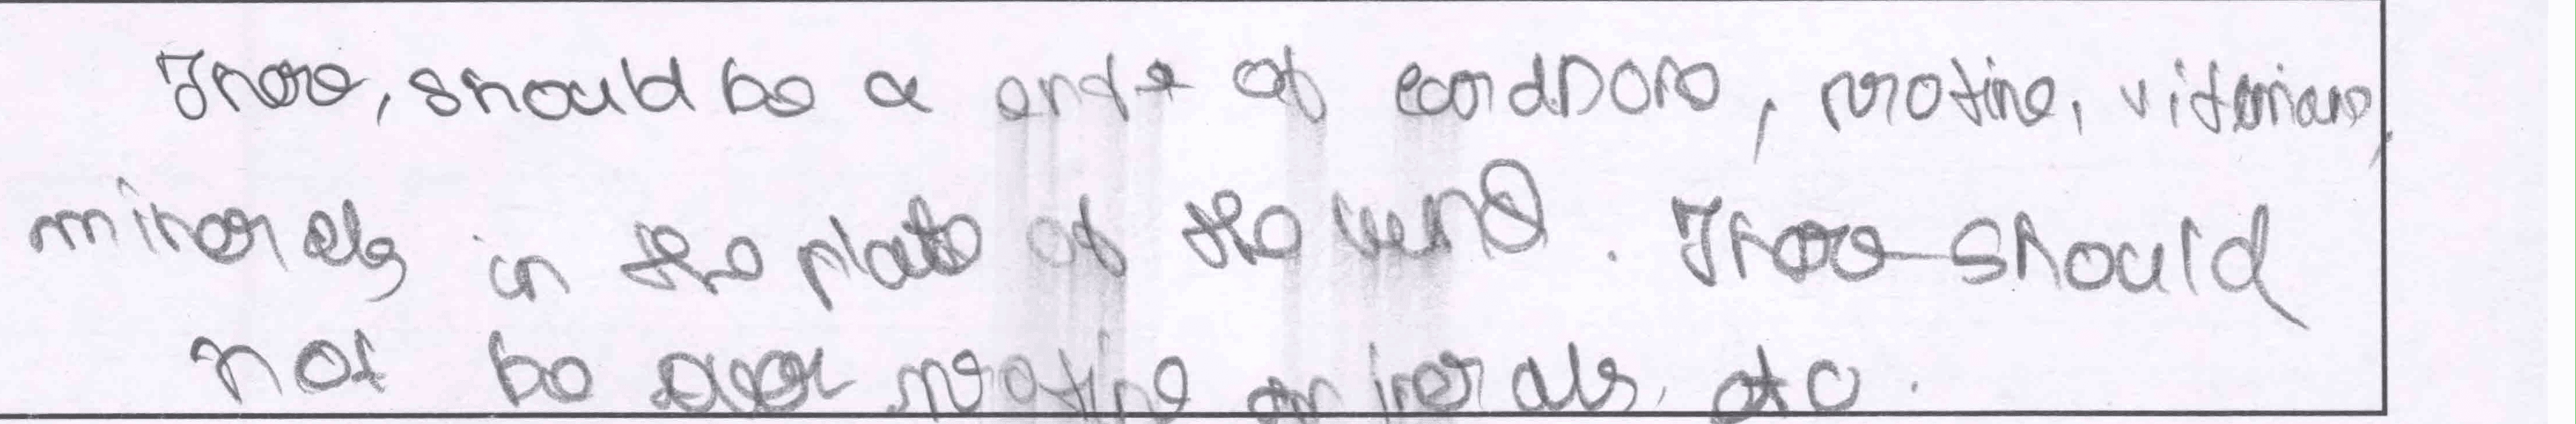
\includegraphics[width=6cm]{Q60_D117170_Science.png}}
    \end{minipage}
    \vspace{10pt}

    % Image: Q60_D117171_Science.png - Scaled height: 3.68mm
    \begin{minipage}{\linewidth}
    \RaggedRight\textbf{\tiny \highgreen{Elakyaa N [D]}} \\ 
    \vspace{4.00pt}\fcolorbox{blue}{white}{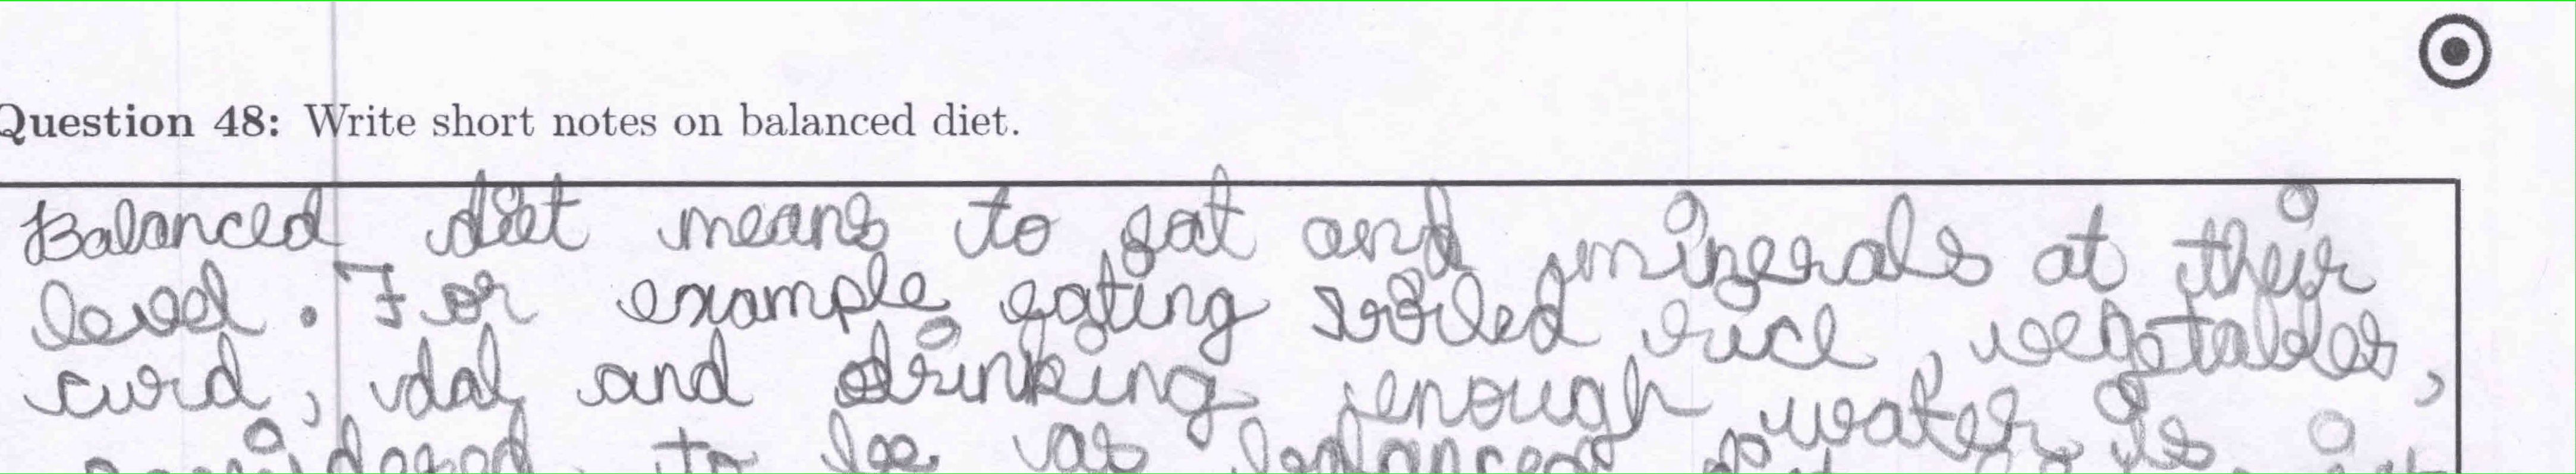
\includegraphics[width=6cm]{Q60_D117171_Science.png}}
    \end{minipage}
    \vspace{10pt}

    % Image: Q60_D117172_Science.png - Scaled height: 3.20mm
    \begin{minipage}{\linewidth}
    \RaggedRight\textbf{\tiny \highgreen{Raksha Nivasini K S [D]}} \\ 
    \vspace{4.00pt}\fcolorbox{blue}{white}{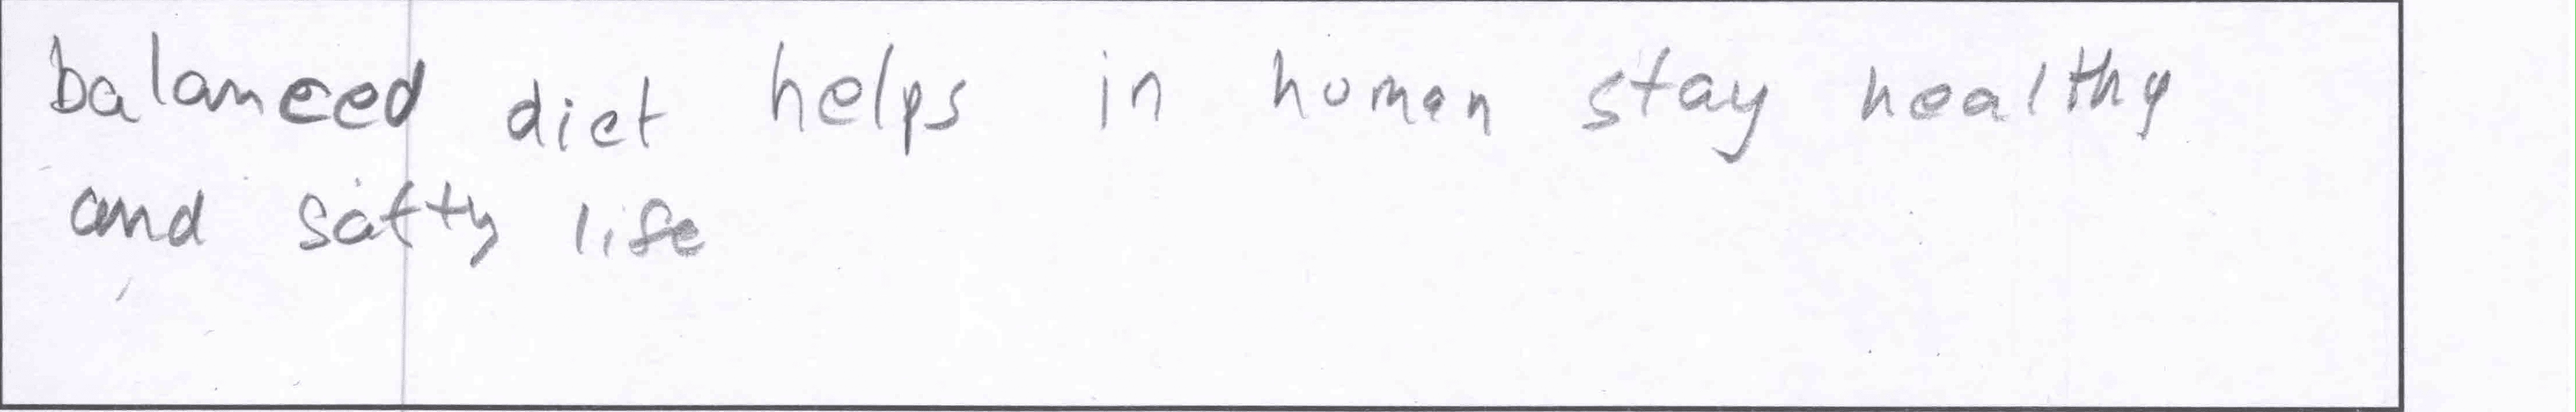
\includegraphics[width=6cm]{Q60_D117172_Science.png}}
    \end{minipage}
    \vspace{10pt}

    % Image: Q60_D117173_Science.png - Scaled height: 3.19mm
    \begin{minipage}{\linewidth}
    \RaggedRight\textbf{\tiny \highred{Sashtika M [B]}} \\ 
    \vspace{4.00pt}\fcolorbox{blue}{white}{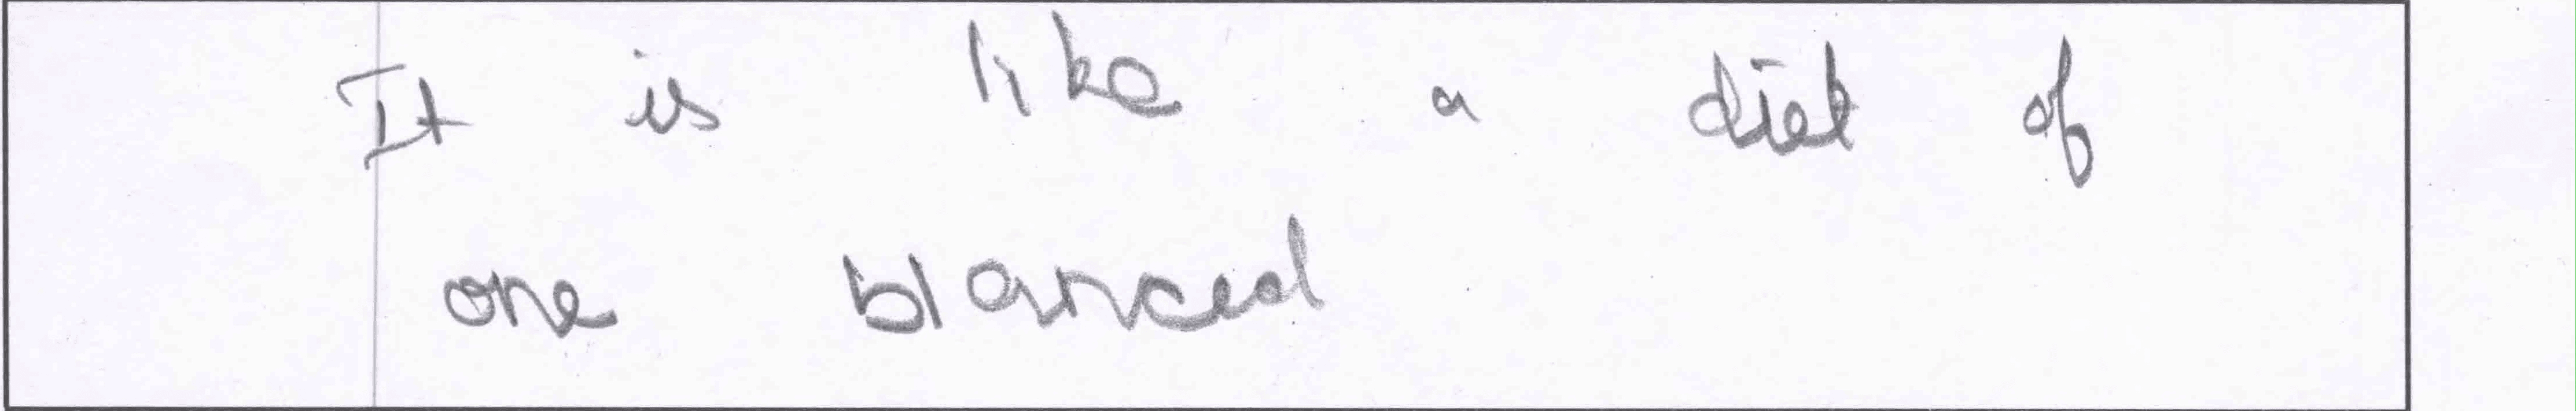
\includegraphics[width=6cm]{Q60_D117173_Science.png}}
    \end{minipage}
    \vspace{10pt}

    % Image: Q60_D117174_Science.png - Scaled height: 3.16mm
    \begin{minipage}{\linewidth}
    \RaggedRight\textbf{\tiny \highred{Sasmithaa R K [B]}} \\ 
    \vspace{4.00pt}\fcolorbox{blue}{white}{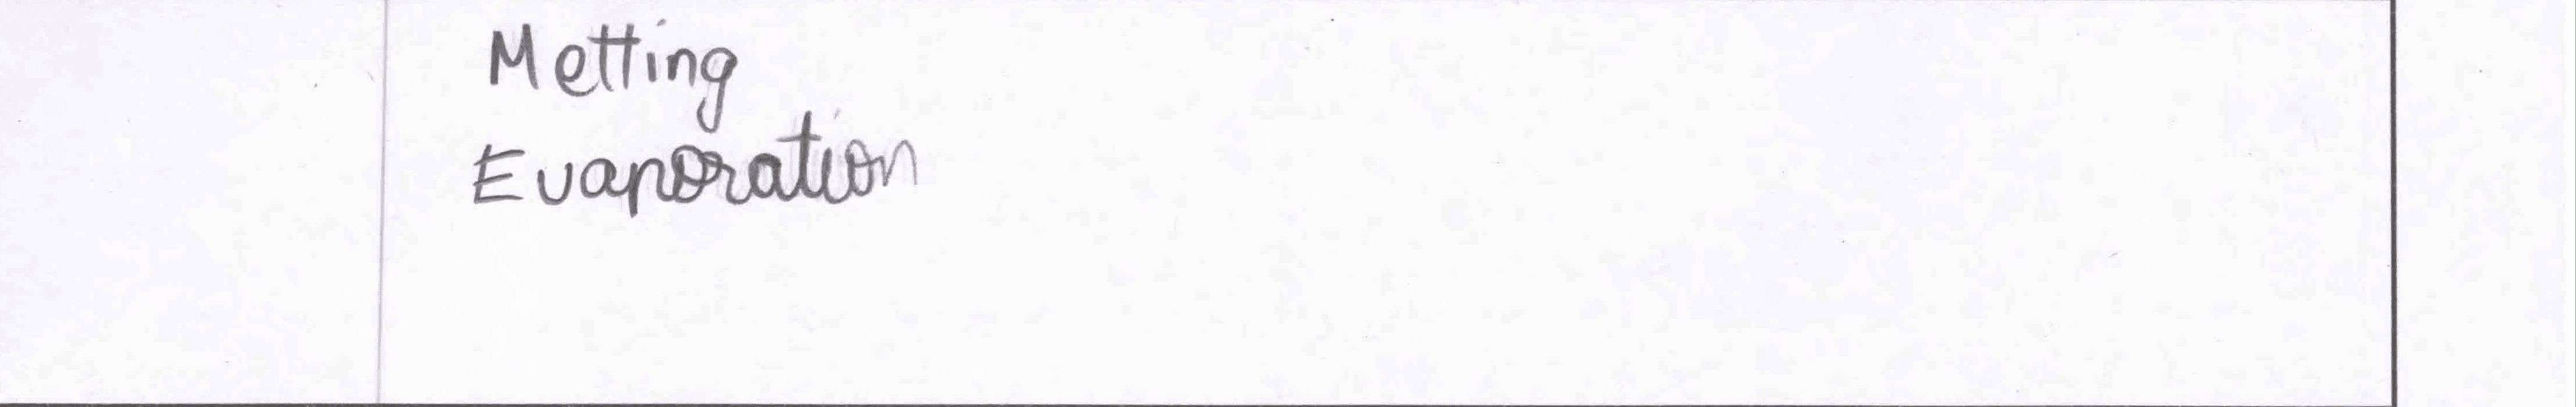
\includegraphics[width=6cm]{Q60_D117174_Science.png}}
    \end{minipage}
    \vspace{10pt}
   \end{multicols}
\end{frame}


\begin{frame}[shrink=0.1,label=QPC6QC6S04 - DT - Q2]{Q27 [2. Sorting Materials into Groups]}
\vspace{-0.2cm}
\mcqtextsideFourOne{
  questionnumber={27},
  questionTag = {C6S04 - DT – Q2},
  questiontext = {Find the incorrect pair based on the object and material used for making it.\\	
  \quad A. Cricket bat – Wood \\	
  \quad B. Lock and key – Metal \\	
  \quad C. Pillow – Cotton \\	
  \quad D. Mirror – Leather \\	
  \quad E. Switch box – Copper},
  optionA={A, B, C},
  optionB={A, D, E},
  optionC={D, E},
  optionD={A, C},
  correctoption={C},
  leftmini = {0.6},
  rightmini = {0.3},
  }

\begin{minipage}{\linewidth}
\hspace{1cm}
\centering
\tiny
\renewcommand{\arraystretch}{1.25}
\begin{tabular}{|M{1.2cm}|M{0.8cm}|M{0.8cm}|M{0.8cm}|M{0.8cm}|M{0.8cm}|}
\hline
Option & A (\ding{55}) & B (\ding{55}) & \cellcolor{cellgreen} C (\ding{51}) & D (\ding{55}) & E \\ 
\hline
6 A & \highno{7\%} & \highno{0\%} & \highgreen{87\%} & \highno{7\%} & \highno{0\%} \\ 
 \hline 
6 B & \highno{5\%} & \highno{5\%} & \highno{63\%} & \highno{21\%} & \highno{5\%} \\ \hline
\end{tabular}
\end{minipage}

\end{frame}
% \input{4. PPT/6. My Answer/Science/C6/117_C6S - Q27}


\begin{frame}[shrink=0.1,label=QPC6QC6S04 - DT - Q7]{Q29 [2. Sorting Materials into Groups]}
\vspace{-0.2cm}
\mcqtextbottomOneFour{
  questionnumber={29}, 
  questiontext={Which of the following is not a property of gold ?},
  optionA={Lustrous },
  optionB={Softness},
  optionC={Insolubility},
  optionD={Sink in water},
  questionTag={C6S04 - DT – Q7}, 
  correctoption={B},
}

\begin{minipage}{\linewidth}
\hspace{1cm}
\centering
\tiny
\renewcommand{\arraystretch}{1.25}
\begin{tabular}{|M{1.2cm}|M{0.8cm}|M{0.8cm}|M{0.8cm}|M{0.8cm}|M{0.8cm}|}
\hline
Option & A (\ding{55}) & \cellcolor{cellgreen} B (\ding{51}) & C (\ding{55}) & D (\ding{55}) & E \\ 
\hline
6 A & \highno{7\%} & \highno{53\%} & \highno{7\%} & \highno{33\%} & \highno{0\%} \\ 
 \hline 
6 B & \highno{11\%} & \highno{47\%} & \highno{21\%} & \highno{21\%} & \highno{0\%} \\ \hline
\end{tabular}
\end{minipage}

\end{frame}
% \input{4. PPT/6. My Answer/Science/C6/117_C6S - Q29}


\begin{frame}[shrink=0.1,label=QPC6QC6S04 - DT - Q8]{Q31 [2. Sorting Materials into Groups]}
\vspace{-0.2cm}
\mcqtextbottomTwoTwo{
  questionnumber={31}, 
  questiontext={Find out the correct pair based on the lustrous property.},
  optionA={Iron – Non-lustrous },
  optionB={Cardboard – Non-lustrous },
  optionC={Jute – Lustrous },
  optionD={Chalk – Lustrous },
  questionTag={C6S04 - DT – Q8}, 
  correctoption={B},
}

\begin{minipage}{\linewidth}
\hspace{1cm}
\centering
\tiny
\renewcommand{\arraystretch}{1.25}
\begin{tabular}{|M{1.2cm}|M{0.8cm}|M{0.8cm}|M{0.8cm}|M{0.8cm}|M{0.8cm}|}
\hline
Option & A (\ding{55}) & \cellcolor{cellgreen} B (\ding{51}) & C (\ding{55}) & D (\ding{55}) & E \\ 
\hline
6 A & \highno{7\%} & \highred{33\%} & \highno{33\%} & \highno{20\%} & \highno{7\%} \\ 
 \hline 
6 B & \highno{42\%} & \highred{21\%} & \highno{16\%} & \highno{16\%} & \highno{5\%} \\ \hline
\end{tabular}
\end{minipage}

\end{frame}
% \input{4. PPT/6. My Answer/Science/C6/117_C6S - Q31}


\begin{frame}[shrink=0.1,label=QPC6QC6S04 - DT - Q5]{Q39 [2. Sorting Materials into Groups]}
\vspace{-0.2cm}
\mcqtextbottomTwoTwo{
  questionnumber={39}, 
  questiontext={Identify the incorrect answer based on the floatation of the object in the water.},
  optionA={Coconut will sink in water },
  optionB={Dry leaf will float in water},
  optionC={Stone will sink in water},
  optionD={Oil will float in water},
  questionTag={C6S04 - DT – Q5}, 
  correctoption={A},
}

\begin{minipage}{\linewidth}
\hspace{1cm}
\centering
\tiny
\renewcommand{\arraystretch}{1.25}
\begin{tabular}{|M{1.2cm}|M{0.8cm}|M{0.8cm}|M{0.8cm}|M{0.8cm}|M{0.8cm}|}
\hline
Option & \cellcolor{cellgreen} A (\ding{51}) & B (\ding{55}) & C (\ding{55}) & D (\ding{55}) & E \\ 
\hline
6 A & \highno{40\%} & \highno{7\%} & \highno{20\%} & \highno{33\%} & \highno{0\%} \\ 
 \hline 
6 B & \highno{63\%} & \highno{11\%} & \highno{0\%} & \highno{21\%} & \highno{5\%} \\ \hline
\end{tabular}
\end{minipage}

\end{frame}
% \input{4. PPT/6. My Answer/Science/C6/117_C6S - Q39}


\begin{frame}[shrink=0.1,label=QPC6QC6S04 - DT - Q15]{Q49 [2. Sorting Materials into Groups]}
\vspace{-0.2cm}



\matextbottomOneFour{
myanswerquestion={Answer the questions based on the solubility of substances.},
myanswercontent={\RaggedRight 
\begin{enumerate}
    \item Salt and sugar dissolve in water, while oil does not dissolve in water. 
    \item Substances that dissolve in water are called \rule{120pt}{0.5pt} substance.
    \item Substances that does not dissolve in water are called \rule{120pt}{0.5pt} substance.
\end{enumerate}
},
questionnumber={49}, 
questionTag={C6S04 - DT - Q15},
questiontext={Identify the soluble substance in water.},
optionA={Wheat grains},
optionB={Sand},
optionC={Stone},
optionD={Coffee powder}, 
correctoption={D},
}


\begin{minipage}{\linewidth}
\hspace{1cm}
\centering
\tiny
\renewcommand{\arraystretch}{1.25}
\begin{tabular}{|M{1.2cm}|M{0.8cm}|M{0.8cm}|M{0.8cm}|M{0.8cm}|M{0.8cm}|}
\hline
Option & A (\ding{55}) & B (\ding{55}) & C (\ding{55}) & \cellcolor{cellgreen} D (\ding{51}) & E \\ 
\hline
6 A & \highno{20\%} & \highno{0\%} & \highno{0\%} & \highgreen{80\%} & \highno{0\%} \\ 
 \hline 
6 B & \highno{11\%} & \highno{16\%} & \highno{5\%} & \highno{63\%} & \highno{5\%} \\ \hline
\end{tabular}
\end{minipage}

\end{frame}
\begin{frame}{Q49 - My Answer Responses}
    \vspace{-0.6cm}
    \begin{multicols}{2}

    % Image: Q49_D117140_Science.png - Scaled height: 2.48mm
    \begin{minipage}{\linewidth}
    \RaggedRight\textbf{\tiny \highgreen{Sabarish B [D]}} \\ 
    \vspace{4.00pt}\fcolorbox{blue}{white}{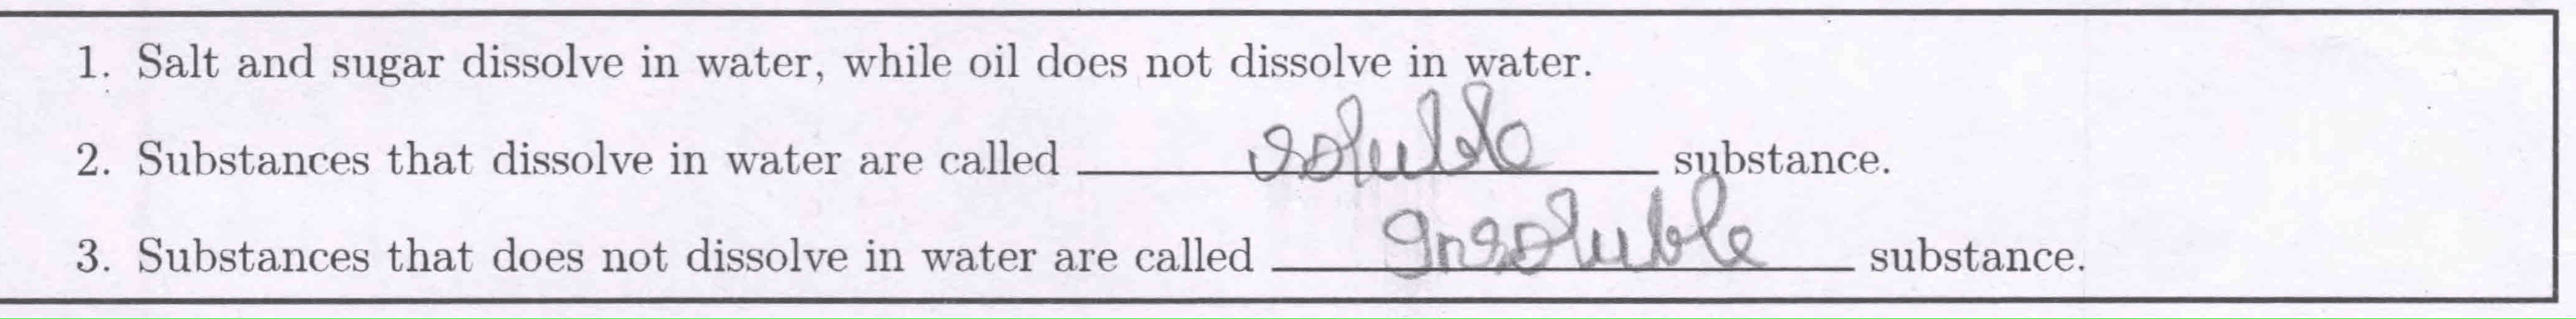
\includegraphics[width=6cm]{Q49_D117140_Science.png}}
    \end{minipage}
    \vspace{10pt}

    % Image: Q49_D117144_Science.png - Scaled height: 2.50mm
    \begin{minipage}{\linewidth}
    \RaggedRight\textbf{\tiny \highgreen{Varshanth K [D]}} \\ 
    \vspace{4.00pt}\fcolorbox{blue}{white}{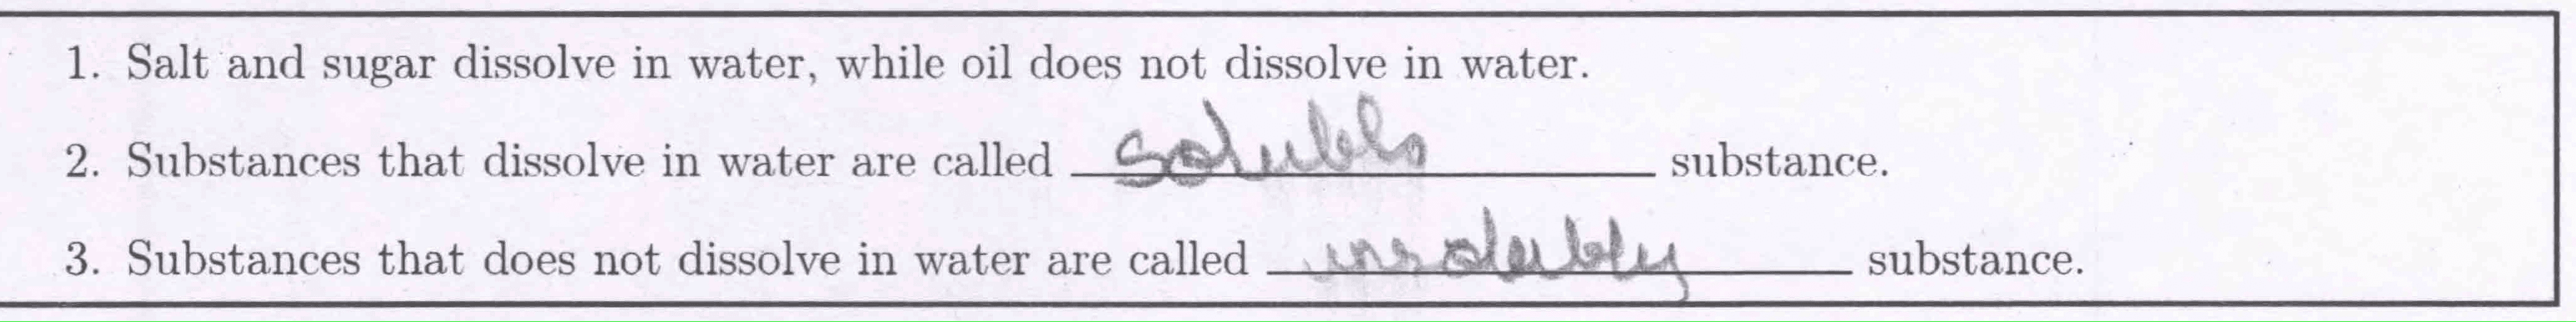
\includegraphics[width=6cm]{Q49_D117144_Science.png}}
    \end{minipage}
    \vspace{10pt}

    % Image: Q49_D117147_Science.png - Scaled height: 2.26mm
    \begin{minipage}{\linewidth}
    \RaggedRight\textbf{\tiny \highred{Anusika M [A]}} \\ 
    \vspace{4.00pt}\fcolorbox{blue}{white}{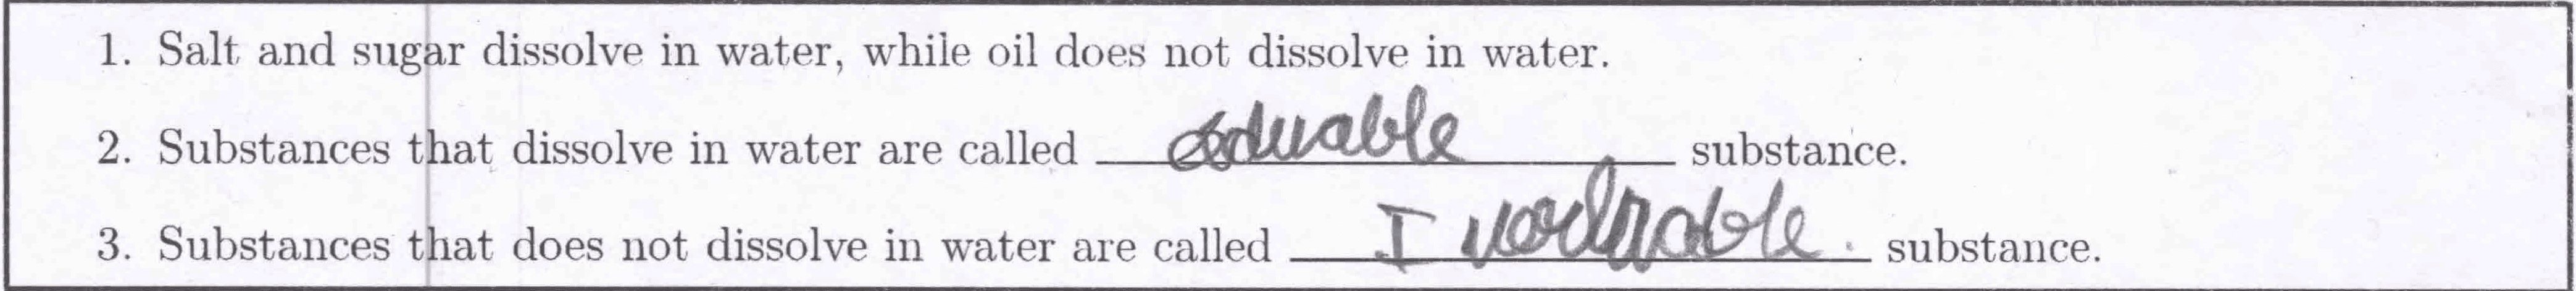
\includegraphics[width=6cm]{Q49_D117147_Science.png}}
    \end{minipage}
    \vspace{10pt}

    % Image: Q49_D117152_Science.png - Scaled height: 2.31mm
    \begin{minipage}{\linewidth}
    \RaggedRight\textbf{\tiny \highgreen{Preethi T [D]}} \\ 
    \vspace{4.00pt}\fcolorbox{blue}{white}{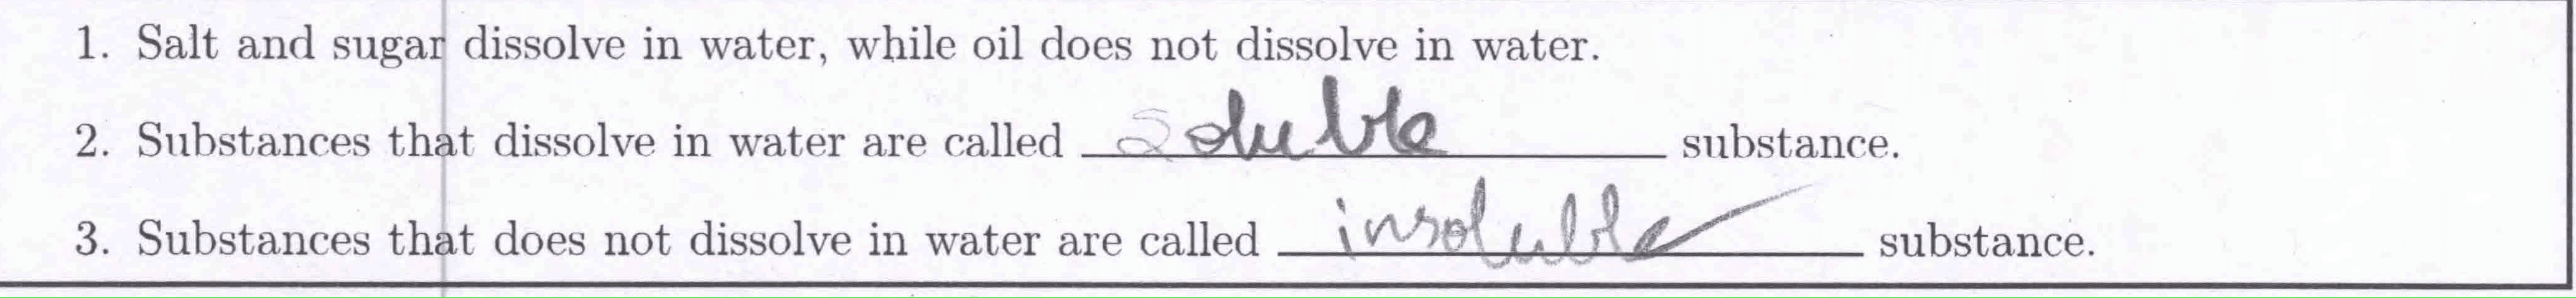
\includegraphics[width=6cm]{Q49_D117152_Science.png}}
    \end{minipage}
    \vspace{10pt}

    % Image: Q49_D117155_Science.png - Scaled height: 2.41mm
    \begin{minipage}{\linewidth}
    \RaggedRight\textbf{\tiny \highred{Sri Nivashini S [A]}} \\ 
    \vspace{4.00pt}\fcolorbox{blue}{white}{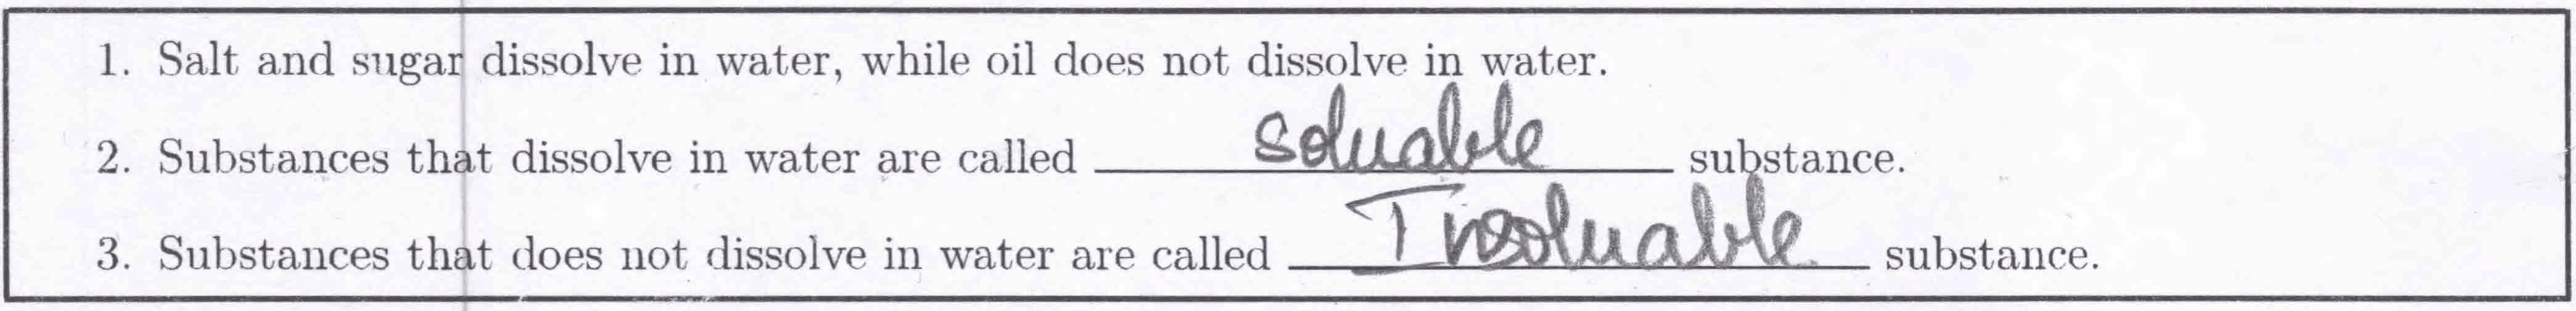
\includegraphics[width=6cm]{Q49_D117155_Science.png}}
    \end{minipage}
    \vspace{10pt}

    % Image: Q49_D117156_Science.png - Scaled height: 2.52mm
    \begin{minipage}{\linewidth}
    \RaggedRight\textbf{\tiny \highgreen{Akil E [D]}} \\ 
    \vspace{4.00pt}\fcolorbox{blue}{white}{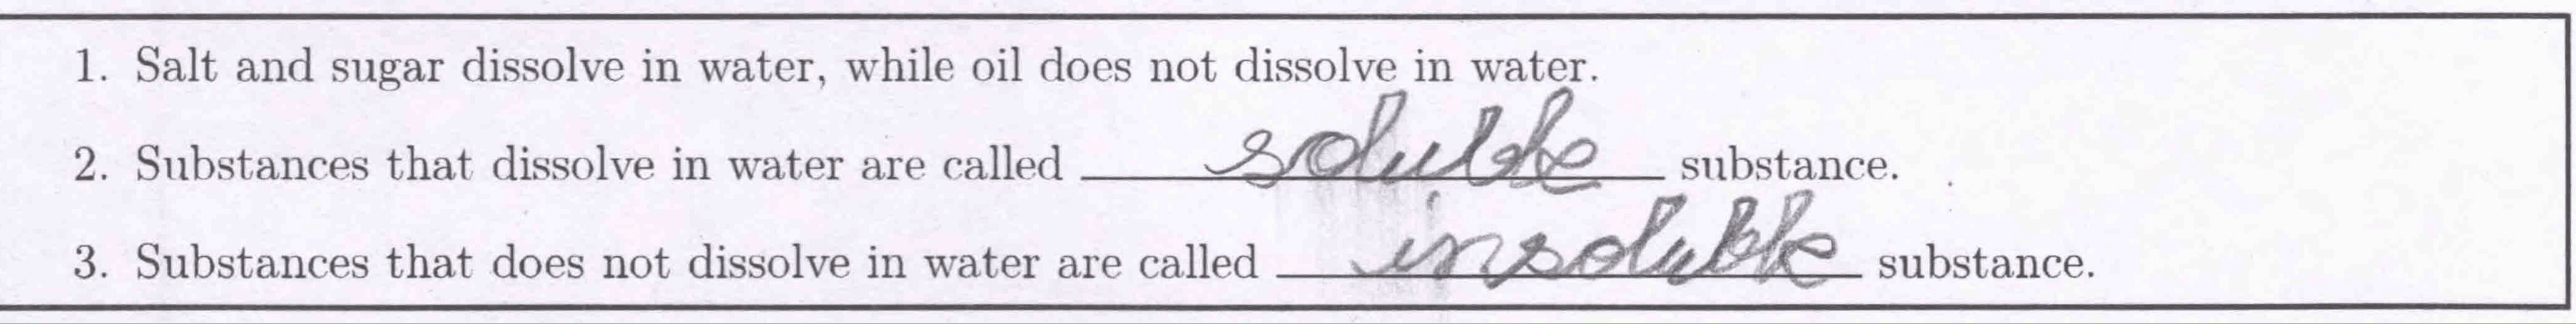
\includegraphics[width=6cm]{Q49_D117156_Science.png}}
    \end{minipage}
    \vspace{10pt}

    % Image: Q49_D117160_Science.png - Scaled height: 2.47mm
    \begin{minipage}{\linewidth}
    \RaggedRight\textbf{\tiny \highred{Hrithik T [A]}} \\ 
    \vspace{4.00pt}\fcolorbox{blue}{white}{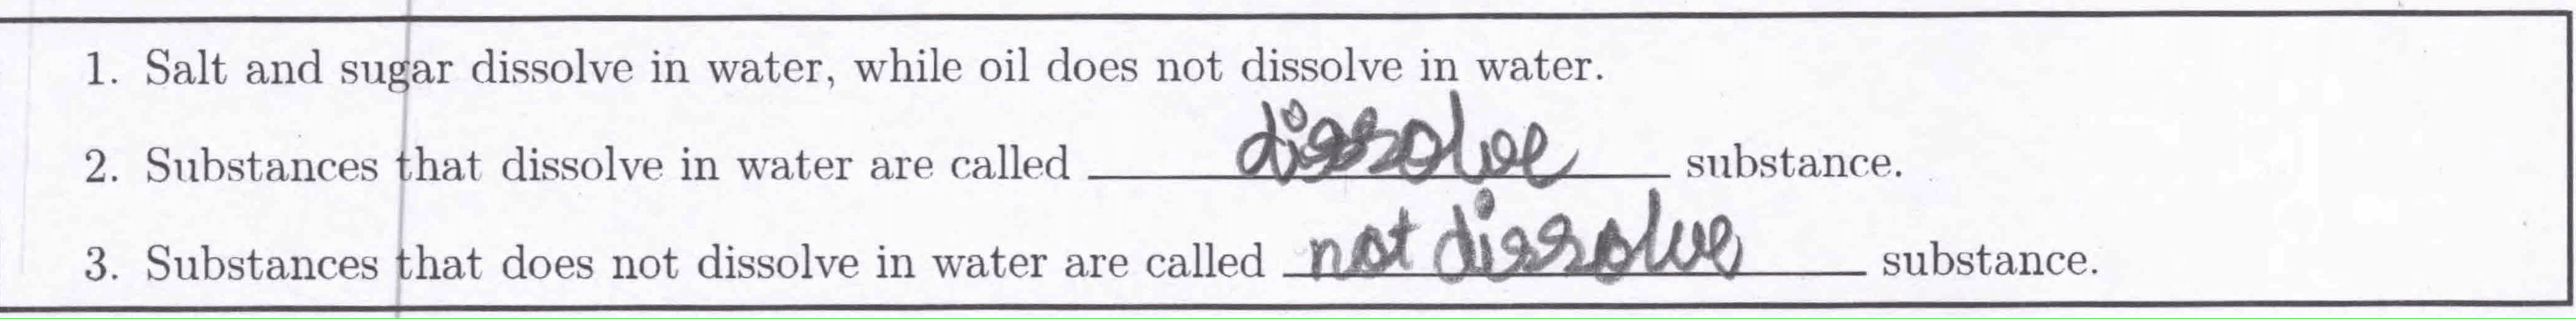
\includegraphics[width=6cm]{Q49_D117160_Science.png}}
    \end{minipage}
    \vspace{10pt}

    
    \end{multicols}
\end{frame}


\begin{frame}{Q49 - My Answer Responses}
    \vspace{-0.6cm}
    \begin{multicols}{2}

% Image: Q49_D117161_Science.png - Scaled height: 2.35mm
    \begin{minipage}{\linewidth}
    \RaggedRight\textbf{\tiny \highgreen{Kiruthik D [D]}} \\ 
    \vspace{4.00pt}\fcolorbox{blue}{white}{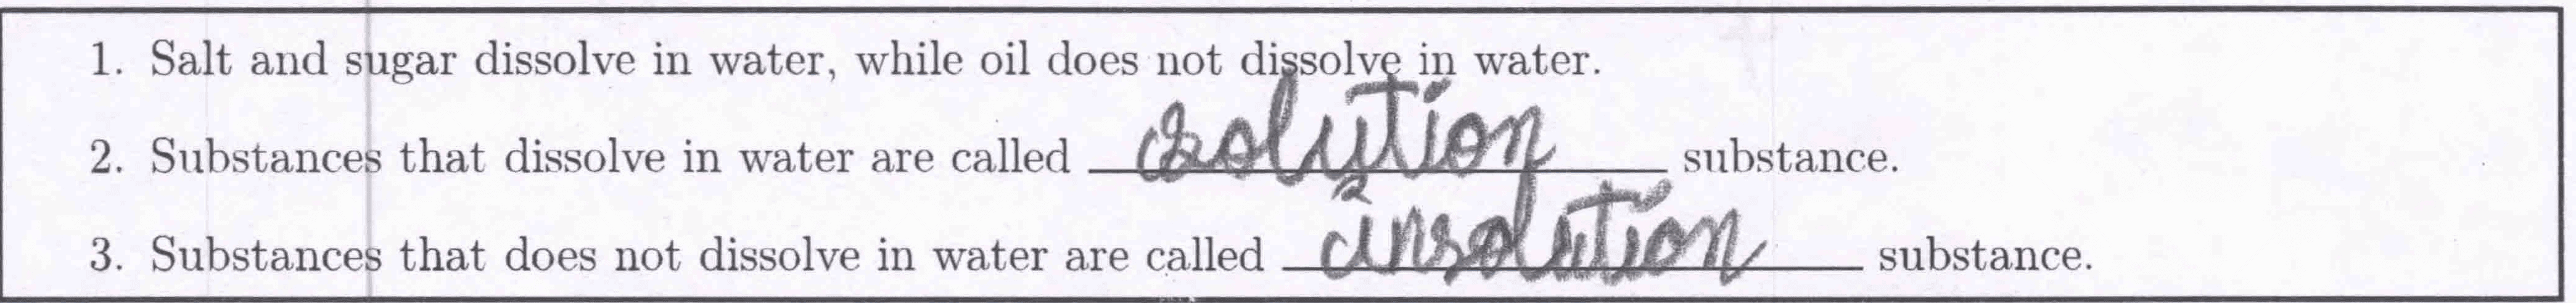
\includegraphics[width=6cm]{Q49_D117161_Science.png}}
    \end{minipage}
    \vspace{10pt}

    % Image: Q49_D117167_Science.png - Scaled height: 2.41mm
    \begin{minipage}{\linewidth}
    \RaggedRight\textbf{\tiny \highgreen{Sriram Karthikeyan V [D]}} \\ 
    \vspace{4.00pt}\fcolorbox{blue}{white}{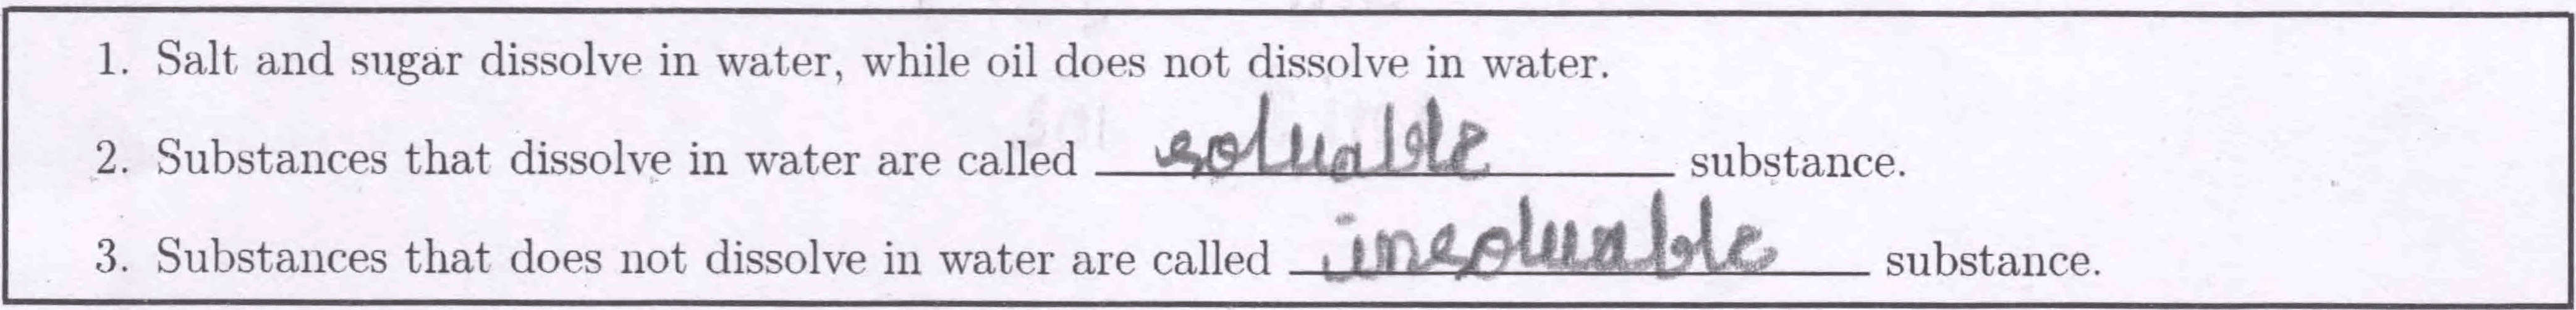
\includegraphics[width=6cm]{Q49_D117167_Science.png}}
    \end{minipage}
    \vspace{10pt}

    % Image: Q49_D117168_Science.png - Scaled height: 2.38mm
    \begin{minipage}{\linewidth}
    \RaggedRight\textbf{\tiny \highgreen{Thirupugazh K A [D]}} \\ 
    \vspace{4.00pt}\fcolorbox{blue}{white}{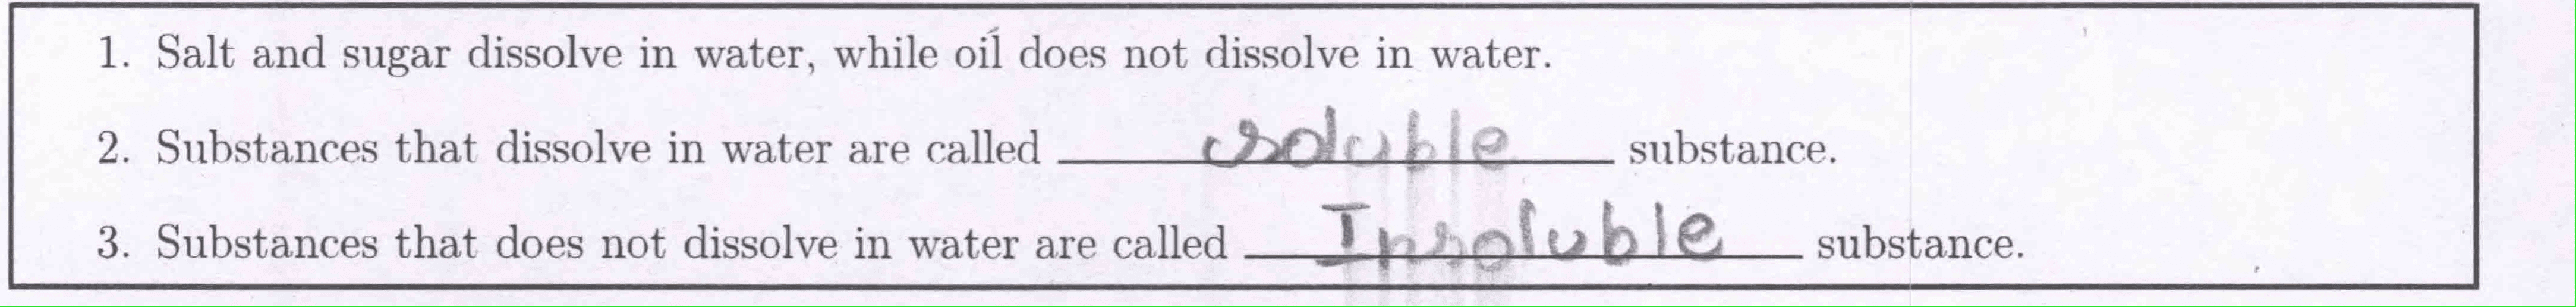
\includegraphics[width=6cm]{Q49_D117168_Science.png}}
    \end{minipage}
    \vspace{10pt}

    % Image: Q49_D117170_Science.png - Scaled height: 2.37mm
    \begin{minipage}{\linewidth}
    \RaggedRight\textbf{\tiny \highred{Cemmozhi S [C]}} \\ 
    \vspace{4.00pt}\fcolorbox{blue}{white}{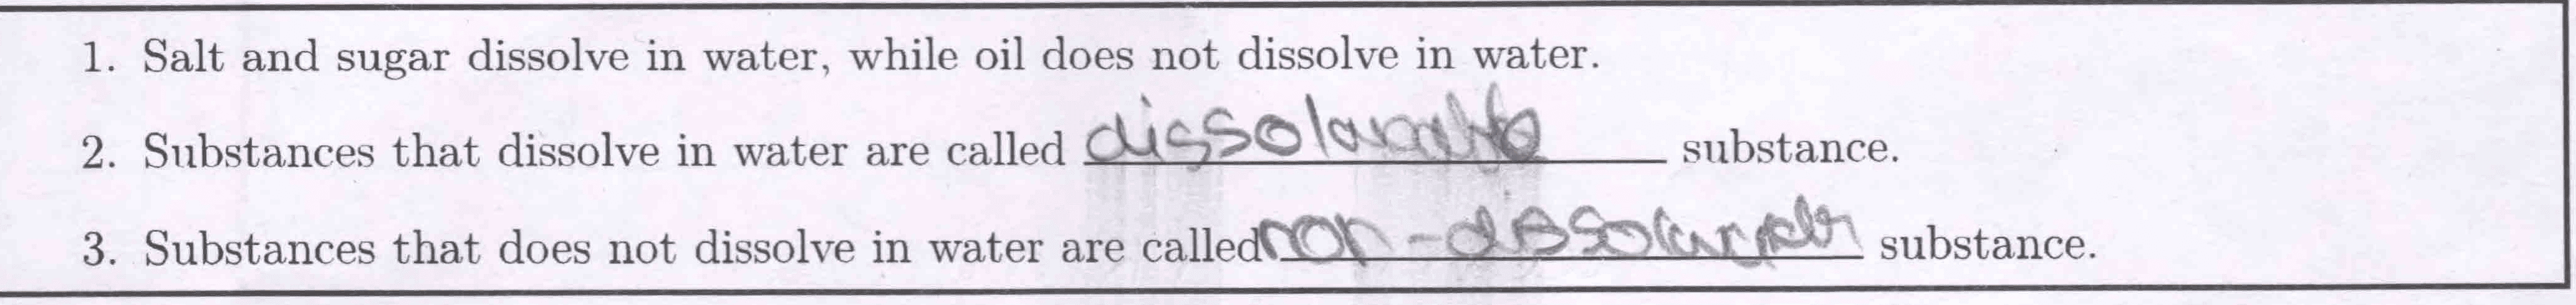
\includegraphics[width=6cm]{Q49_D117170_Science.png}}
    \end{minipage}
    \vspace{10pt}

    % Image: Q49_D117171_Science.png - Scaled height: 2.45mm
    \begin{minipage}{\linewidth}
    \RaggedRight\textbf{\tiny \highgreen{Elakyaa N [D]}} \\ 
    \vspace{4.00pt}\fcolorbox{blue}{white}{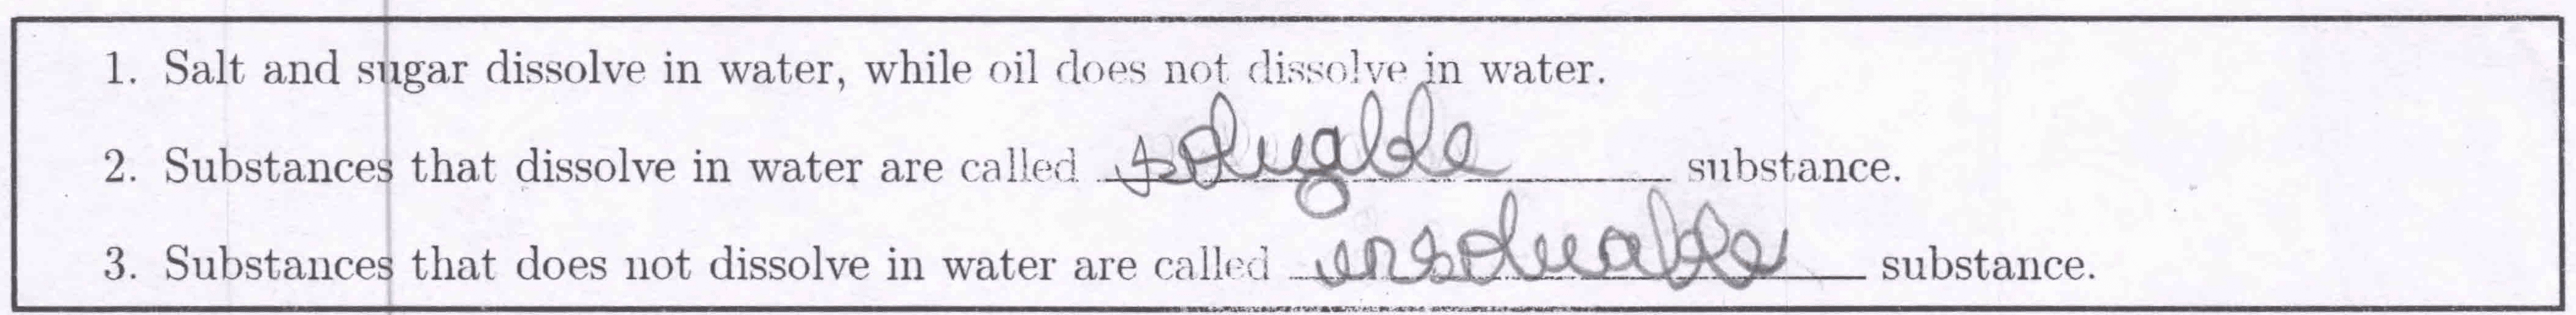
\includegraphics[width=6cm]{Q49_D117171_Science.png}}
    \end{minipage}
    \vspace{10pt}

    % Image: Q49_D117172_Science.png - Scaled height: 2.29mm
    \begin{minipage}{\linewidth}
    \RaggedRight\textbf{\tiny \highgreen{Raksha Nivasini K S [D]}} \\ 
    \vspace{4.00pt}\fcolorbox{blue}{white}{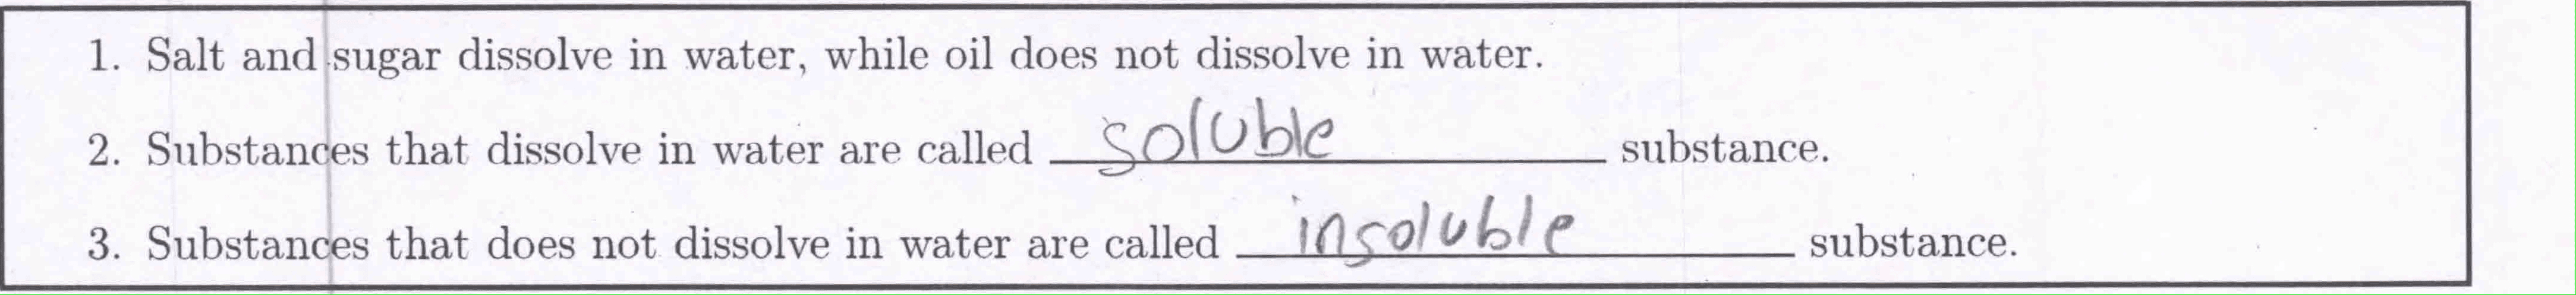
\includegraphics[width=6cm]{Q49_D117172_Science.png}}
    \end{minipage}
    \vspace{10pt}

    % Image: Q49_D117173_Science.png - Scaled height: 2.43mm
    \begin{minipage}{\linewidth}
    \RaggedRight\textbf{\tiny \highgreen{Sashtika M [D]}} \\ 
    \vspace{4.00pt}\fcolorbox{blue}{white}{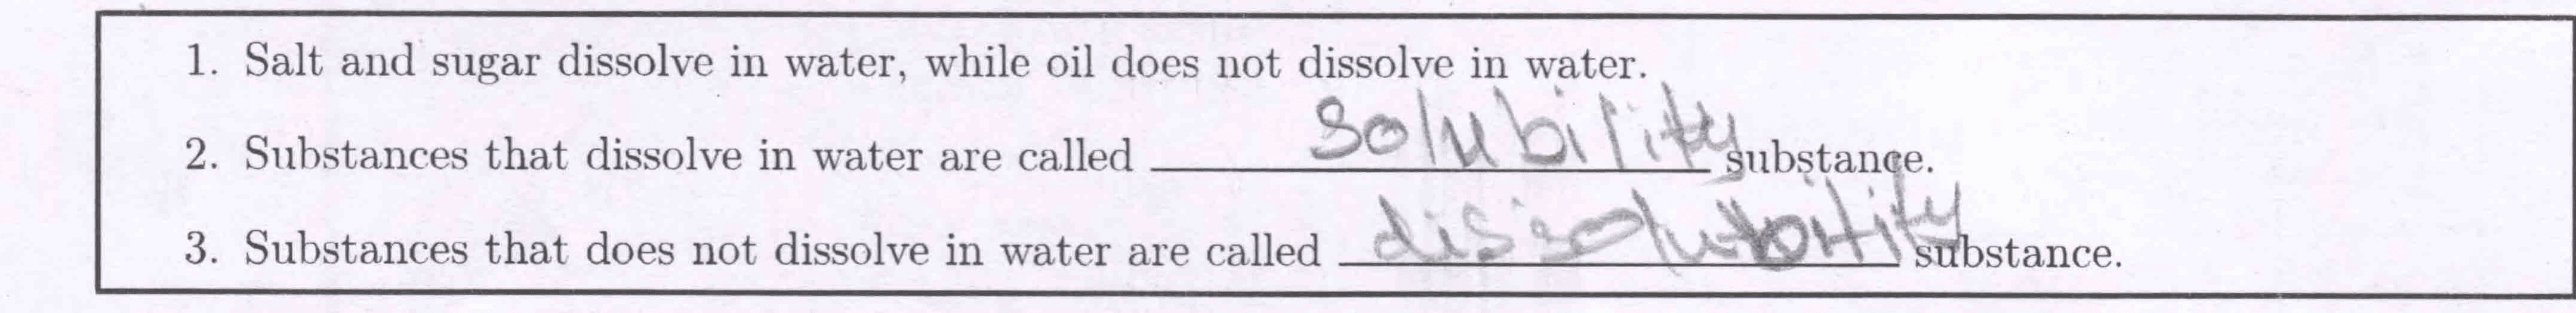
\includegraphics[width=6cm]{Q49_D117173_Science.png}}
    \end{minipage}
    \vspace{10pt}

    % Image: Q49_D117174_Science.png - Scaled height: 2.44mm
    \begin{minipage}{\linewidth}
    \RaggedRight\textbf{\tiny \highred{Sasmithaa R K [B]}} \\ 
    \vspace{4.00pt}\fcolorbox{blue}{white}{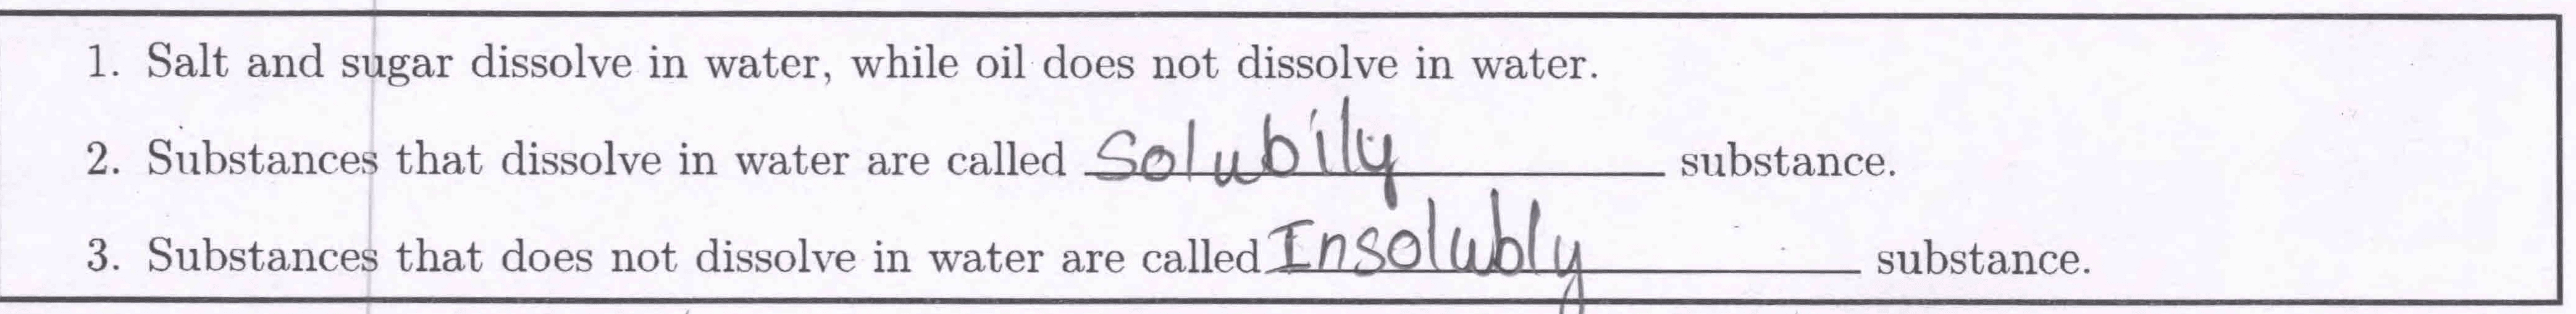
\includegraphics[width=6cm]{Q49_D117174_Science.png}}
    \end{minipage}
    \vspace{10pt}

 \end{multicols}
\end{frame}


\begin{frame}[shrink=0.1,label=QPC6QC6S05 - DT - Q9]{Q6 [3. Separation of Substances]}
\vspace{-0.2cm}
\mcqtextbottomTwoTwo{
  questionnumber={6}, 
  questiontext={\\i. The solution in which two spoons of sugar are dissolved in a glass of water is called \rule{60pt}{0.1pt} solution.
  \\ii. The solution in which ten spoons of sugar are dissolved in a glass of water and no more sugar can be dissolved in it is called \rule{60pt}{0.1pt} solution.},
  optionA={Unsaturated, Saturated},
  optionB={Saturated, Unsaturated},
  optionC={Supersaturated, Unsaturated},
  optionD={Saturated, Supersaturated},
  questionTag={C6S05 - DT – Q9}, 
  correctoption={A},
}

\begin{minipage}{\linewidth}
\hspace{1cm}
\centering
\tiny
\renewcommand{\arraystretch}{1.25}
\begin{tabular}{|M{1.2cm}|M{0.8cm}|M{0.8cm}|M{0.8cm}|M{0.8cm}|M{0.8cm}|}
\hline
Option & \cellcolor{cellgreen} A (\ding{51}) & B (\ding{55}) & C (\ding{55}) & D (\ding{55}) & E \\ 
\hline
6 A & \highno{40\%} & \highno{47\%} & \highno{7\%} & \highno{7\%} & \highno{0\%} \\ 
 \hline 
6 B & \highred{26\%} & \highno{47\%} & \highno{11\%} & \highno{16\%} & \highno{0\%} \\ \hline
\end{tabular}
\end{minipage}

\end{frame}
% \input{4. PPT/6. My Answer/Science/C6/117_C6S - Q6}


\begin{frame}[shrink=0.1,label=QPC6QC6S05 - DT - Q15]{Q16 [3. Separation of Substances]}
\vspace{-0.2cm}

\mcqtextbottomOneFour{
  questionnumber={16}, 
  questionTag={C6S05 - DT – Q15 }, 
  questiontext={While cooking, Raj’s mother accidentally poured some water into the oil can. Now, she needs to separate the oil from the water in the mixture. How can she do this?},
  optionA={Churning},
  optionB={Decantation},
  optionC={Sedimentation},
  optionD={Winnowing},
  correctoption={B},
}

\begin{minipage}{\linewidth}
\hspace{1cm}
\centering
\tiny
\renewcommand{\arraystretch}{1.25}
\begin{tabular}{|M{1.2cm}|M{0.8cm}|M{0.8cm}|M{0.8cm}|M{0.8cm}|M{0.8cm}|}
\hline
Option & A (\ding{55}) & \cellcolor{cellgreen} B (\ding{51}) & C (\ding{55}) & D (\ding{55}) & E \\ 
\hline
6 A & \highno{0\%} & \highno{53\%} & \highno{33\%} & \highno{13\%} & \highno{0\%} \\ 
 \hline 
6 B & \highno{16\%} & \highred{37\%} & \highno{37\%} & \highno{11\%} & \highno{0\%} \\ \hline
\end{tabular}
\end{minipage}

\end{frame}
% \input{4. PPT/6. My Answer/Science/C6/117_C6S - Q16}


\begin{frame}[shrink=0.1,label=QPC6QC6S05 - DT - Q10]{Q21 [3. Separation of Substances]}
\vspace{-0.2cm}
\mcqimgleftFourOne{
  questionnumber={21}, 
  questiontext={Ravi mixes oil with water and milk with water in two different glasses. Identify the liquid that is soluble in water.},
  imgtabletikz = {

\tikzset{every picture/.style={line width=0.75pt,scale=\scalefactor}} % set default line width to 0.75pt        
\begin{tikzpicture}[x=0.75pt,y=0.75pt,yscale=-1,xscale=1]
\draw (125,55) node  {\adjustbox{scale=\scalefactor}{\includegraphics[width=52.5pt,height=62.5pt]{C6S05 - DT – Q10i.png}}};
\draw (265,56) node  {\adjustbox{scale=\scalefactor}{\includegraphics[width=52.5pt,height=62.5pt]{C6S05 - DT – Q10ii.jpg}}};
\draw (83,103) node [anchor=north west][inner sep=0.75pt]   [align=left] {Oil and Water};
\draw (218,103) node [anchor=north west][inner sep=0.75pt]   [align=left] {Milk and Water};
\end{tikzpicture}
},
  optionA={Oil is soluble in water. },
  optionB={Milk is soluble in water. },
  optionC={Both oil and milk are soluble in water.},
  optionD={Both oil and milk are insoluble in water.},
  questionTag={C6S05 - DT – Q10},
  leftmini={0.4},
  rightmini={0.5},
  correctoption={B},
}

\begin{minipage}{\linewidth}
\hspace{1cm}
\centering
\tiny
\renewcommand{\arraystretch}{1.25}
\begin{tabular}{|M{1.2cm}|M{0.8cm}|M{0.8cm}|M{0.8cm}|M{0.8cm}|M{0.8cm}|}
\hline
Option & A (\ding{55}) & \cellcolor{cellgreen} B (\ding{51}) & C (\ding{55}) & D (\ding{55}) & E \\ 
\hline
6 A & \highno{7\%} & \highno{73\%} & \highno{7\%} & \highno{13\%} & \highno{0\%} \\ 
 \hline 
6 B & \highno{21\%} & \highno{53\%} & \highno{5\%} & \highno{21\%} & \highno{0\%} \\ \hline
\end{tabular}
\end{minipage}

\end{frame}
% \input{4. PPT/6. My Answer/Science/C6/117_C6S - Q21}


\begin{frame}[shrink=0.1,label=QPC6QC6S05 - DT - Q13]{Q37 [3. Separation of Substances]}
\vspace{-0.2cm}

\mcqtextbottomTwoTwo{
  questionnumber={37}, 
  questionTag={C6S05 - DT – Q13}, 
  questiontext={Laila wants to collect clean water from muddy water. Which method of separation should she use?},
  optionA={Decantation},
  optionB={Filtration},
  optionC={Magnetic separation},
  optionD={Sieving},
  correctoption={B},
}


\begin{minipage}{\linewidth}
\hspace{1cm}
\centering
\tiny
\renewcommand{\arraystretch}{1.25}
\begin{tabular}{|M{1.2cm}|M{0.8cm}|M{0.8cm}|M{0.8cm}|M{0.8cm}|M{0.8cm}|}
\hline
Option & A (\ding{55}) & \cellcolor{cellgreen} B (\ding{51}) & C (\ding{55}) & D (\ding{55}) & E \\ 
\hline
6 A & \highno{27\%} & \highno{40\%} & \highno{20\%} & \highno{13\%} & \highno{0\%} \\ 
 \hline 
6 B & \highno{26\%} & \highno{68\%} & \highno{5\%} & \highno{0\%} & \highno{0\%} \\ \hline
\end{tabular}
\end{minipage}

\end{frame}
% \input{4. PPT/6. My Answer/Science/C6/117_C6S - Q37}


\begin{frame}[shrink=0.1,label=QPC6QC6S05 - DT - Q18]{Q57 [3. Separation of Substances]}
\vspace{-0.2cm}


\matextbottomOneFour{
myanswerquestion={Complete the table with the name of the processes that change the state of water.},
myanswercontent={
\centering
\renewcommand{\arraystretch}{1.5}
\begin{tabular}{|>{\centering\arraybackslash}p{5.5cm}|>{\centering\arraybackslash}p{5.5cm}|}
\hline
\textbf{Change in state of water} & \textbf{Process is called} \\
\hline
Water turns to ice &  \\
\hline
Water turns to gas &  \\
\hline
Ice turns to water &  \\
\hline
Gas turns to water &  Condensation\\
\hline
\end{tabular}\\
},
questionnumber={57}, 
questionTag={C6S05 - DT - Q18},
questiontext={Which process helps in drying clothes under the sun?},
optionA={Freezing},
optionB={Melting},
optionC={Condensation},
optionD={Evaporation}, 
correctoption={D},
}

\begin{minipage}{\linewidth}
\hspace{1cm}
\centering
\tiny
\renewcommand{\arraystretch}{1.25}
\begin{tabular}{|M{1.2cm}|M{0.8cm}|M{0.8cm}|M{0.8cm}|M{0.8cm}|M{0.8cm}|}
\hline
Option & A (\ding{55}) & B (\ding{55}) & C (\ding{55}) & \cellcolor{cellgreen} D (\ding{51}) & E \\ 
\hline
6 A & \highno{7\%} & \highno{20\%} & \highno{27\%} & \highno{40\%} & \highno{7\%} \\ 
 \hline 
6 B & \highno{0\%} & \highno{16\%} & \highno{26\%} & \highno{58\%} & \highno{0\%} \\ \hline
\end{tabular}
\end{minipage}

\end{frame}
\begin{frame}{Q57 - My Answer Responses}
    \vspace{-0.6cm}
    \begin{multicols}{2}

    % Image: Q57_D117135_Science.png - Scaled height: 3.72mm
    \begin{minipage}{\linewidth}
    \RaggedRight\textbf{\tiny \highgreen{Dheeresh J A [D]}} \\ 
    \vspace{4.00pt}\fcolorbox{blue}{white}{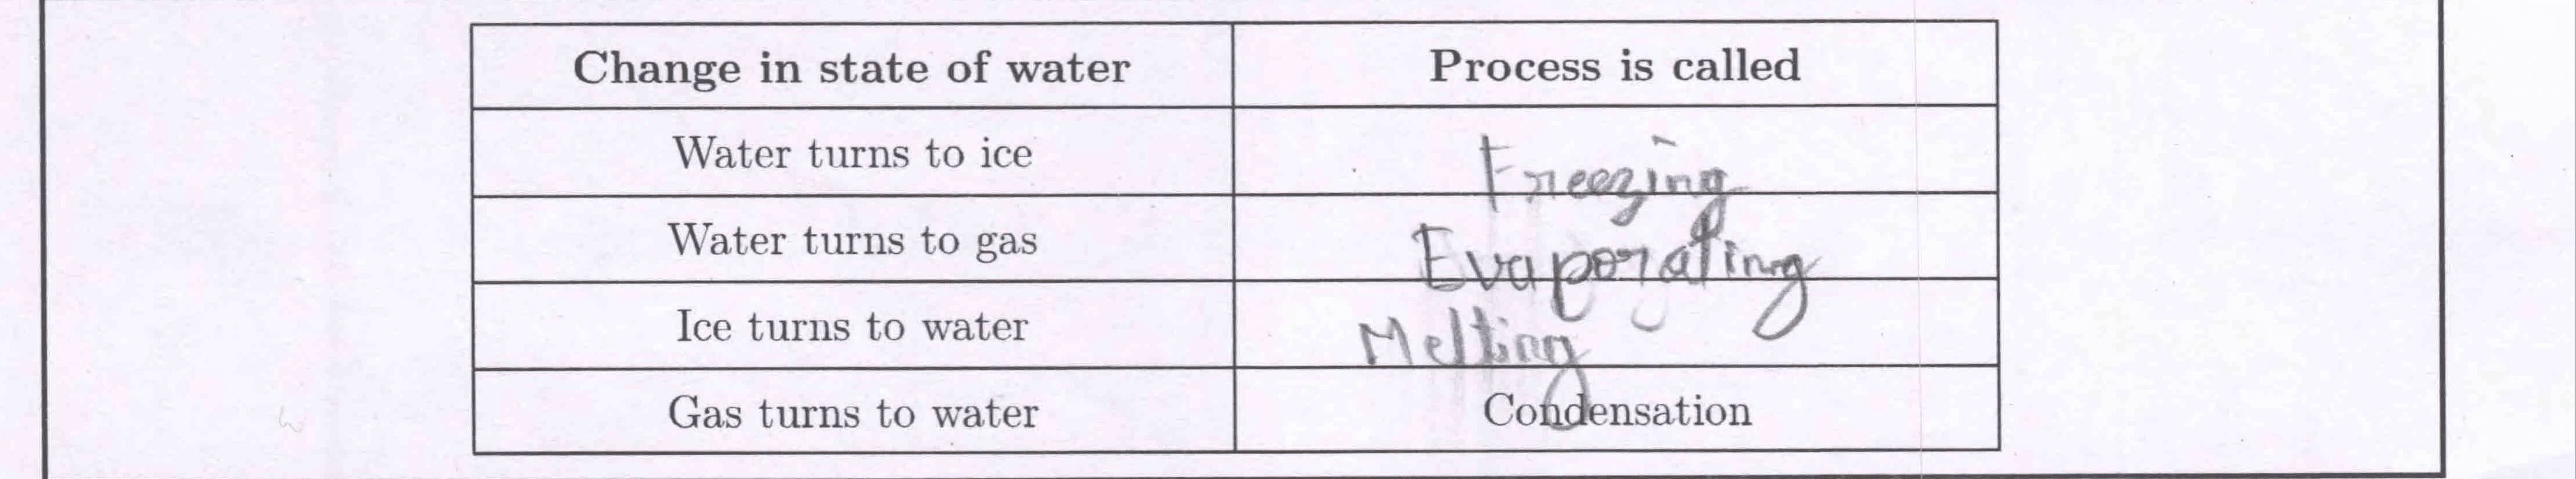
\includegraphics[width=6cm]{Q57_D117135_Science.png}}
    \end{minipage}
    \vspace{10pt}

    % Image: Q57_D117144_Science.png - Scaled height: 5.60mm
    \begin{minipage}{\linewidth}
    \RaggedRight\textbf{\tiny \highred{Varshanth K [B]}} \\ 
    \vspace{4.00pt}\fcolorbox{blue}{white}{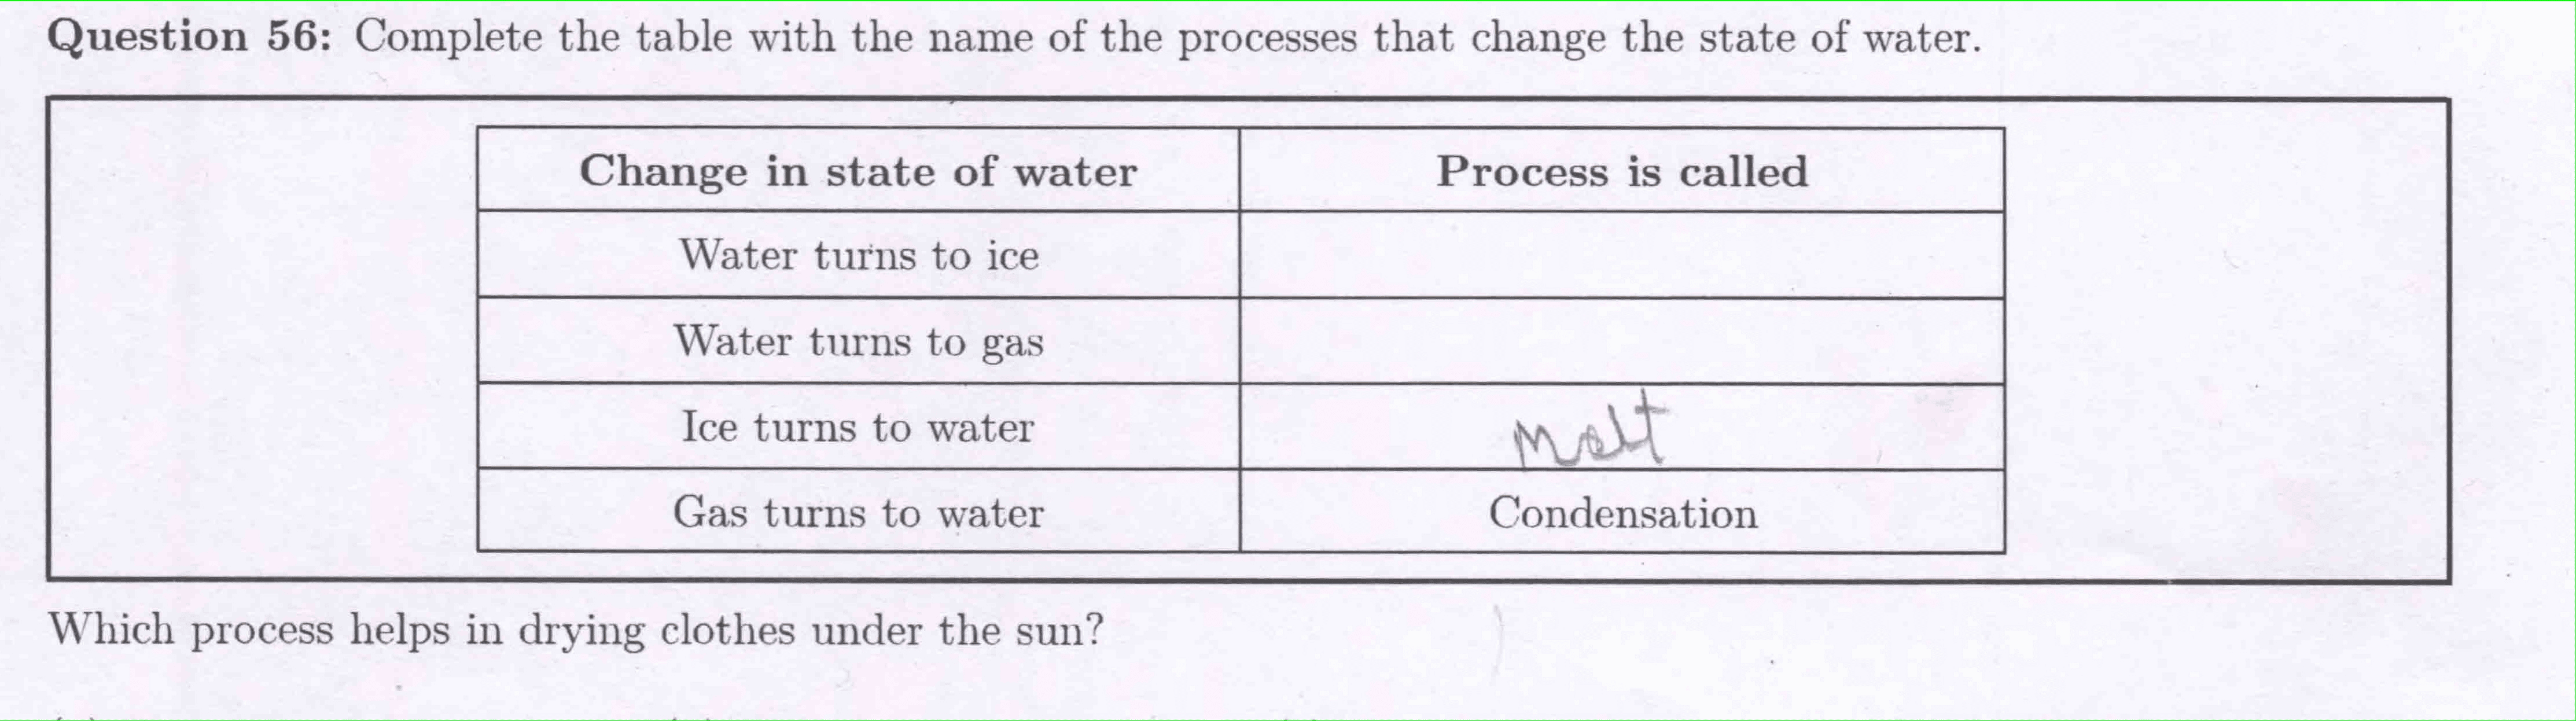
\includegraphics[width=6cm]{Q57_D117144_Science.png}}
    \end{minipage}
    \vspace{10pt}

    % Image: Q57_D117147_Science.png - Scaled height: 3.77mm
    \begin{minipage}{\linewidth}
    \RaggedRight\textbf{\tiny \highgreen{Anusika M [D]}} \\ 
    \vspace{4.00pt}\fcolorbox{blue}{white}{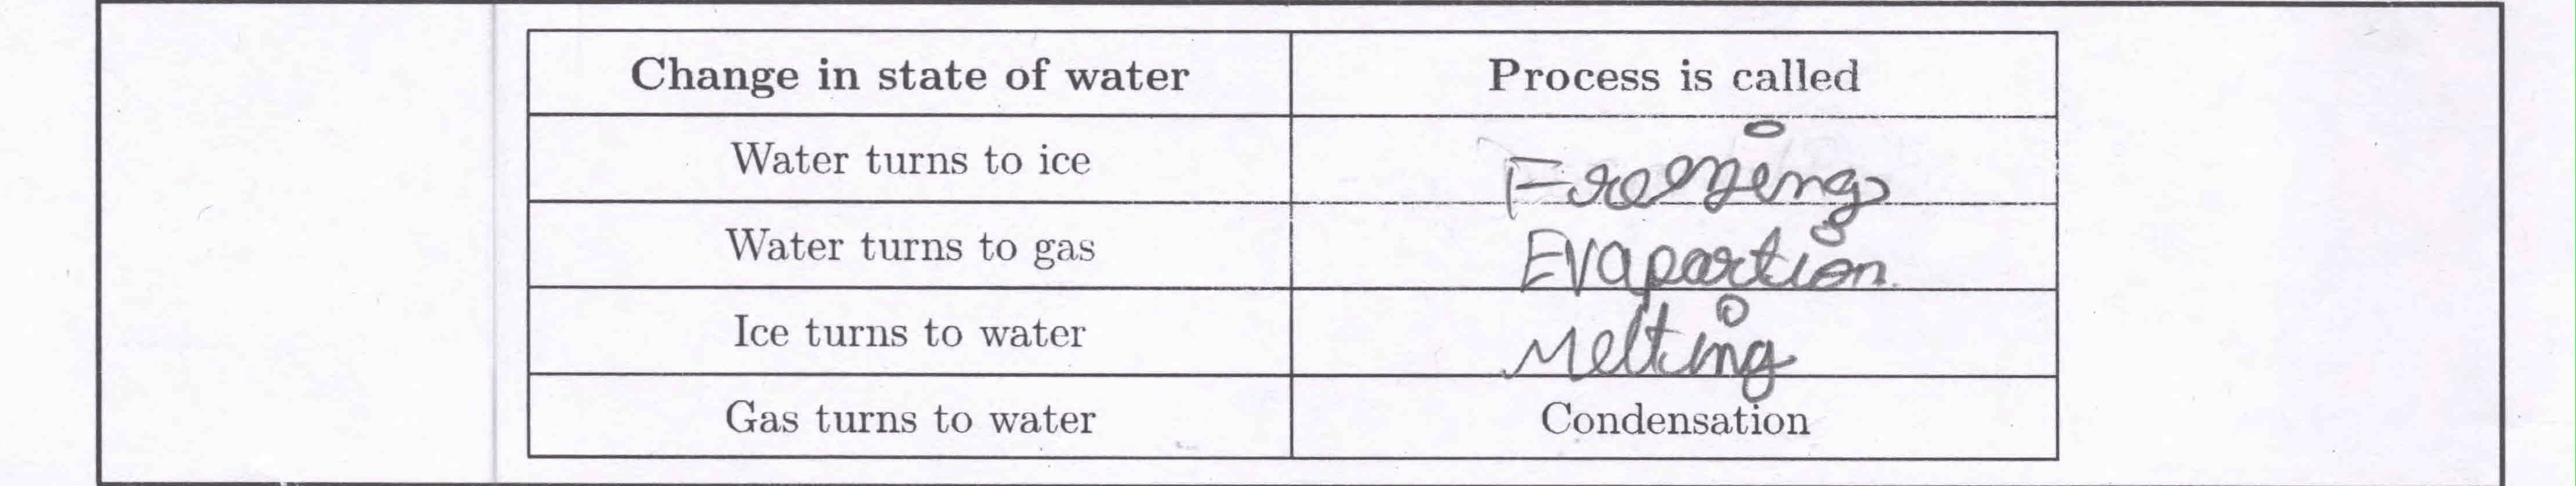
\includegraphics[width=6cm]{Q57_D117147_Science.png}}
    \end{minipage}
    \vspace{10pt}

    % Image: Q57_D117151_Science.png - Scaled height: 4.65mm
    \begin{minipage}{\linewidth}
    \RaggedRight\textbf{\tiny \highred{Karnika R [C]}} \\ 
    \vspace{4.00pt}\fcolorbox{blue}{white}{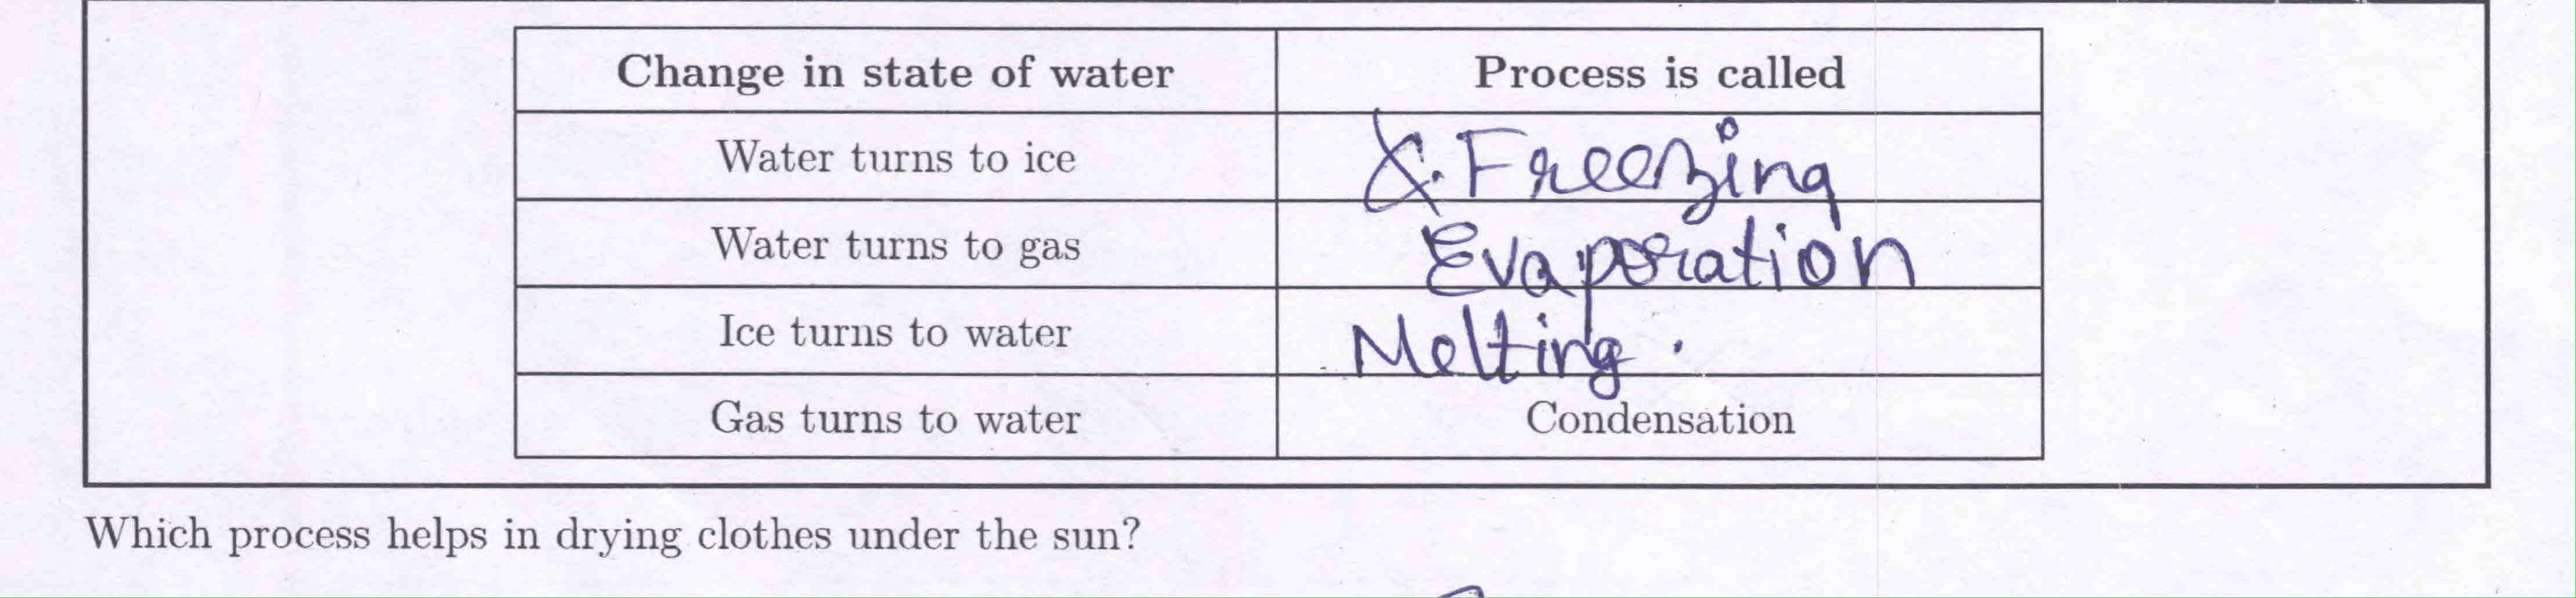
\includegraphics[width=6cm]{Q57_D117151_Science.png}}
    \end{minipage}
    \vspace{10pt}

    % Image: Q57_D117155_Science.png - Scaled height: 3.75mm
    \begin{minipage}{\linewidth}
    \RaggedRight\textbf{\tiny \highgreen{Sri Nivashini S [D]}} \\ 
    \vspace{4.00pt}\fcolorbox{blue}{white}{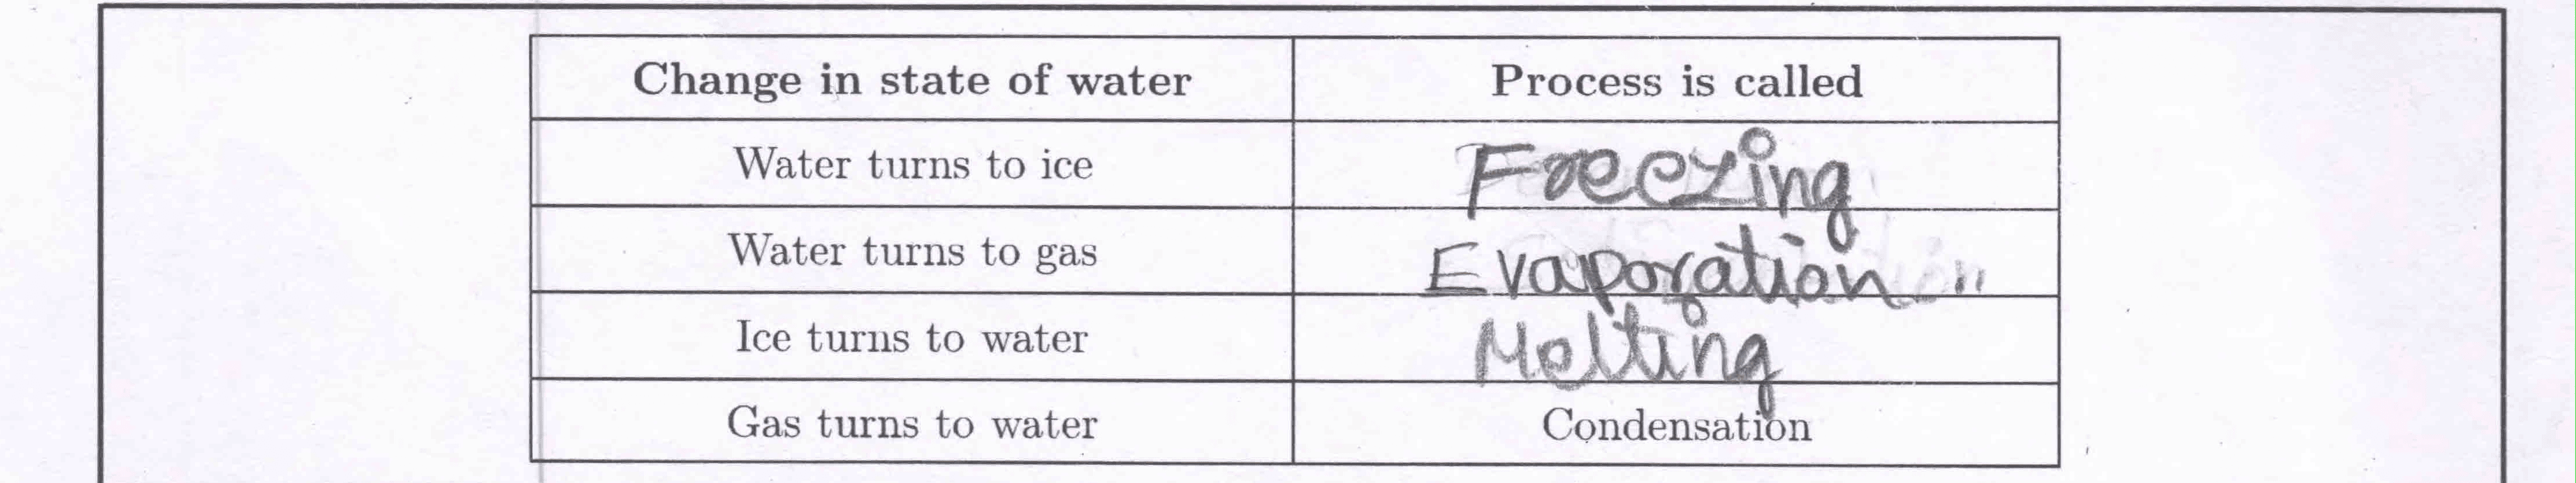
\includegraphics[width=6cm]{Q57_D117155_Science.png}}
    \end{minipage}
    \vspace{10pt}

    % Image: Q57_D117156_Science.png - Scaled height: 3.80mm
    \begin{minipage}{\linewidth}
    \RaggedRight\textbf{\tiny \highgreen{Akil E [D]}} \\ 
    \vspace{4.00pt}\fcolorbox{blue}{white}{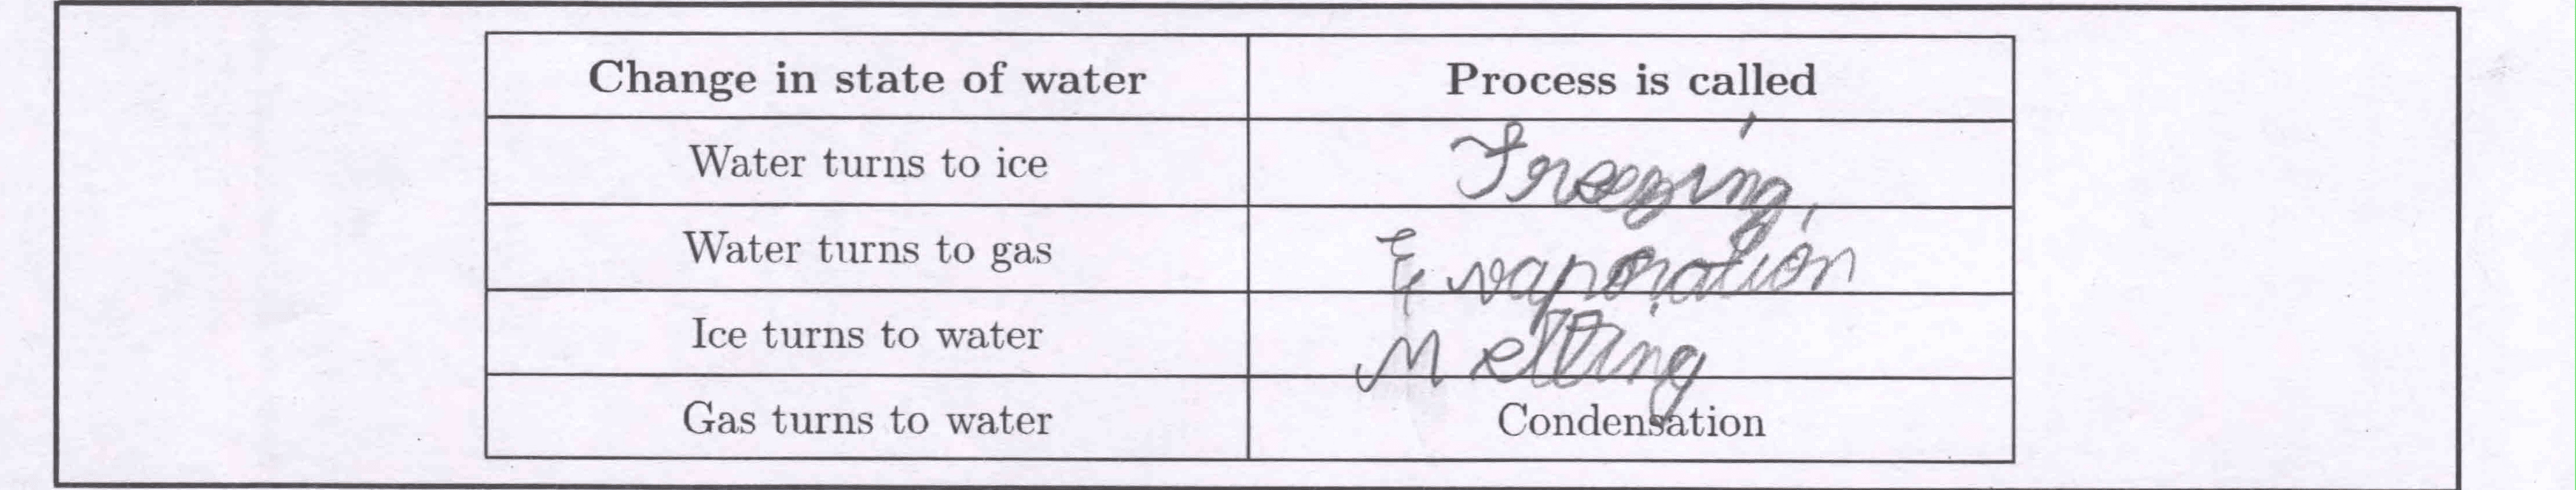
\includegraphics[width=6cm]{Q57_D117156_Science.png}}
    \end{minipage}
    \vspace{10pt}

   
    \end{multicols}
\end{frame}

\begin{frame}{Q57 - My Answer Responses}
    \vspace{-0.6cm}
    \begin{multicols}{2}
 % Image: Q57_D117159_Science.png - Scaled height: 6.98mm
   
    % Image: Q57_D117161_Science.png - Scaled height: 3.85mm
    \begin{minipage}{\linewidth}
    \RaggedRight\textbf{\tiny \highgreen{Kiruthik D [D]}} \\ 
    \vspace{4.00pt}\fcolorbox{blue}{white}{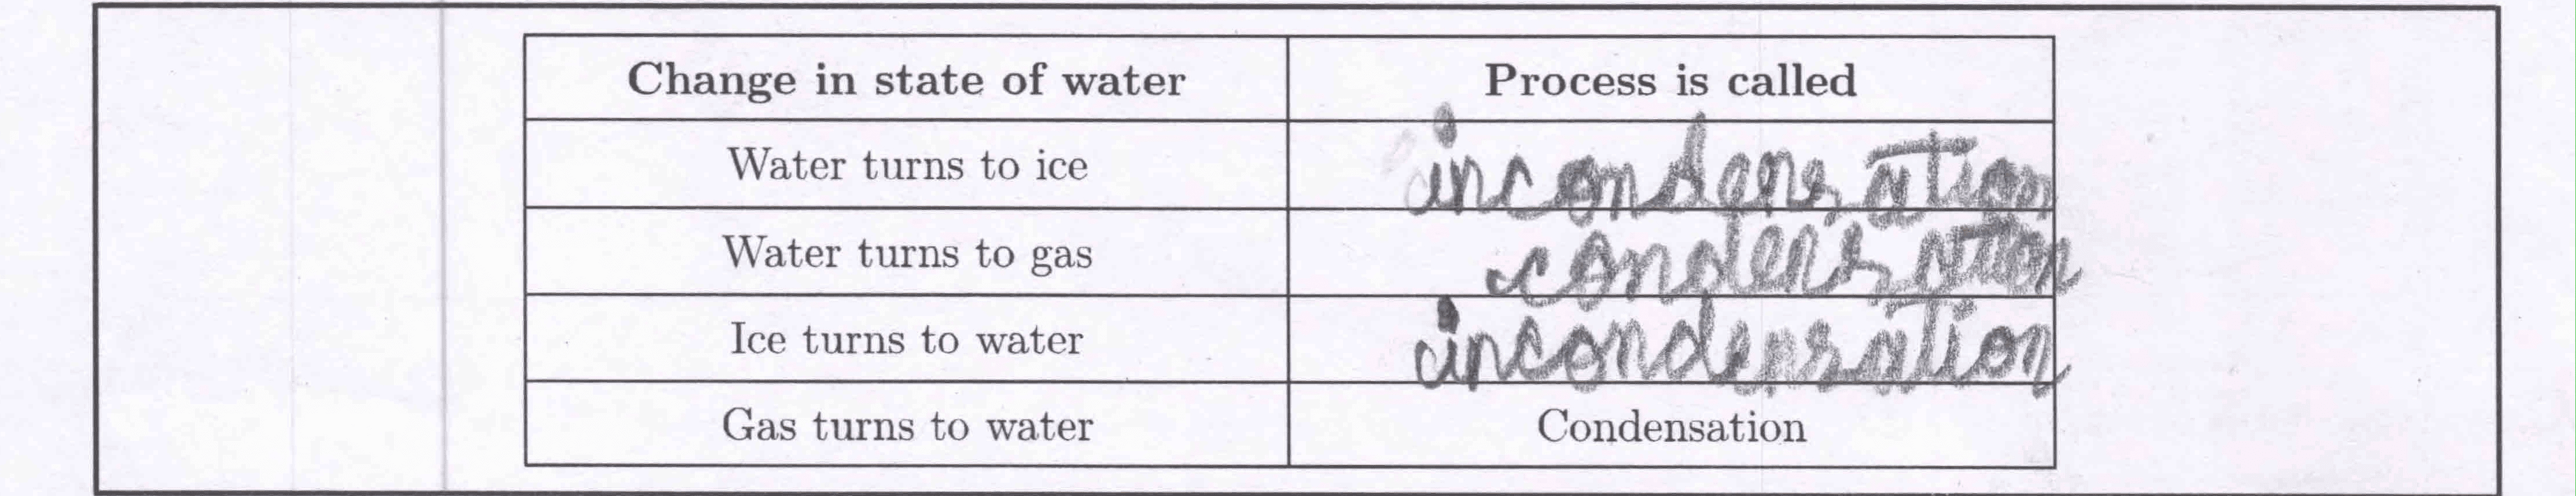
\includegraphics[width=6cm]{Q57_D117161_Science.png}}
    \end{minipage}
    \vspace{10pt}


    % Image: Q57_D117167_Science.png - Scaled height: 3.75mm
    \begin{minipage}{\linewidth}
    \RaggedRight\textbf{\tiny \highgreen{Sriram Karthikeyan V [D]}} \\ 
    \vspace{4.00pt}\fcolorbox{blue}{white}{\includegraphics[width=6cm]{Q57_D117167_Science.png}}
    \end{minipage}
    \vspace{10pt}

    % Image: Q57_D117169_Science.png - Scaled height: 3.73mm
    \begin{minipage}{\linewidth}
    \RaggedRight\textbf{\tiny \highred{Avanthika S [B]}} \\ 
    \vspace{4.00pt}\fcolorbox{blue}{white}{\includegraphics[width=6cm]{Q57_D117169_Science.png}}
    \end{minipage}
    \vspace{10pt}

    % Image: Q57_D117171_Science.png - Scaled height: 3.86mm
    \begin{minipage}{\linewidth}
    \RaggedRight\textbf{\tiny \highgreen{Elakyaa N [D]}} \\ 
    \vspace{4.00pt}\fcolorbox{blue}{white}{\includegraphics[width=6cm]{Q57_D117171_Science.png}}
    \end{minipage}
    \vspace{10pt}

    % Image: Q57_D117172_Science.png - Scaled height: 3.80mm
    \begin{minipage}{\linewidth}
    \RaggedRight\textbf{\tiny \highred{Raksha Nivasini K S [C]}} \\ 
    \vspace{4.00pt}\fcolorbox{blue}{white}{\includegraphics[width=6cm]{Q57_D117172_Science.png}}
    \end{minipage}
    \vspace{10pt}

    % Image: Q57_D117173_Science.png - Scaled height: 6.34mm
    \begin{minipage}{\linewidth}
    \RaggedRight\textbf{\tiny \highred{Sashtika M [C]}} \\ 
    \vspace{4.00pt}\fcolorbox{blue}{white}{\includegraphics[width=6cm]{Q57_D117173_Science.png}}
    \end{minipage}
    \vspace{10pt}

   

   \end{multicols}
\end{frame}


\begin{frame}[shrink=0.1,label=QPC6QC6S07 - DT - Q7]{Q5 [4. Getting to Know Plants]}
\vspace{-0.2cm}
\mcqtextbottomFourOne{
  questionnumber={5}, 
  questiontext={Identify the substance that moves in the upward and downward directions in the plant stem.},
  optionA={Upward direction – Water, Downward direction – Food },
  optionB={Upward direction – Water, Downward direction – Fat },
  optionC={Upward direction – Protein, Downward direction – Water },
  optionD={Upward direction – Food, Downward direction – Water },
  questionTag={C6S07 - DT – Q7}, 
  correctoption={A},
}

\begin{minipage}{\linewidth}
\hspace{1cm}
\centering
\tiny
\renewcommand{\arraystretch}{1.25}
\begin{tabular}{|M{1.2cm}|M{0.8cm}|M{0.8cm}|M{0.8cm}|M{0.8cm}|M{0.8cm}|}
\hline
Option & \cellcolor{cellgreen} A (\ding{51}) & B (\ding{55}) & C (\ding{55}) & D (\ding{55}) & E \\ 
\hline
6 A & \highno{60\%} & \highno{13\%} & \highno{0\%} & \highno{20\%} & \highno{7\%} \\ 
 \hline 
6 B & \highred{37\%} & \highno{5\%} & \highno{11\%} & \highno{37\%} & \highno{11\%} \\ \hline
\end{tabular}
\end{minipage}

\end{frame}
% \input{4. PPT/6. My Answer/Science/C6/117_C6S - Q5}


\begin{frame}[shrink=0.1,label=QPC6QC6S07 - DT - Q1]{Q14 [4. Getting to Know Plants]}
\vspace{-0.2cm}
\mcqimgleftFourOne{
  questionnumber={14}, 
  questiontext={Identify the parts marked in the given plant.},
  imgtabletikz = { {\adjustbox{scale=\scalefactor}{\includegraphics[width=4cm,height=3cm]{C6S07 - DT – Q1.png}}} },
  optionA={1-Leaf system, 2-Root},
  optionB={1-Shoot system, 2-Stem },
  optionC={1-Root system, 2-Root },
  optionD={1-Shoot system, 2-Root},
  questionTag={C6S07 - DT – Q1}, 
  leftmini={0.4},
  rightmini={0.5},
  correctoption={D},
}

\begin{minipage}{\linewidth}
\hspace{1cm}
\centering
\tiny
\renewcommand{\arraystretch}{1.25}
\begin{tabular}{|M{1.2cm}|M{0.8cm}|M{0.8cm}|M{0.8cm}|M{0.8cm}|M{0.8cm}|}
\hline
Option & A (\ding{55}) & B (\ding{55}) & C (\ding{55}) & \cellcolor{cellgreen} D (\ding{51}) & E \\ 
\hline
6 A & \highno{27\%} & \highno{0\%} & \highno{7\%} & \highno{67\%} & \highno{0\%} \\ 
 \hline 
6 B & \highno{16\%} & \highno{5\%} & \highno{5\%} & \highno{68\%} & \highno{5\%} \\ \hline
\end{tabular}
\end{minipage}

\end{frame}
% \input{4. PPT/6. My Answer/Science/C6/117_C6S - Q14}


\begin{frame}[shrink=0.1,label=QPC6QC6S07 - DT - Q9]{Q15 [4. Getting to Know Plants]}
\vspace{-0.2cm}
\mcqtextbottomTwoTwo{
  questionnumber={15}, 
  questiontext={During the process of photosynthesis, \rule{60pt}{0.1pt} gas enters the plant and \rule{60pt}{0.1pt} gas comes out of the plant.},
  optionA={Carbon dioxide, Oxygen},
  optionB={Nitrogen, Carbon dioxide},
  optionC={Oxygen, Carbon dioxide},
  optionD={Nitrogen, Oxygen },
  questionTag={C6S07 - DT – Q9}, 
  correctoption={A},
}

\begin{minipage}{\linewidth}
\hspace{1cm}
\centering
\tiny
\renewcommand{\arraystretch}{1.25}
\begin{tabular}{|M{1.2cm}|M{0.8cm}|M{0.8cm}|M{0.8cm}|M{0.8cm}|M{0.8cm}|}
\hline
Option & \cellcolor{cellgreen} A (\ding{51}) & B (\ding{55}) & C (\ding{55}) & D (\ding{55}) & E \\ 
\hline
6 A & \highgreen{87\%} & \highno{7\%} & \highno{0\%} & \highno{7\%} & \highno{0\%} \\ 
 \hline 
6 B & \highgreen{84\%} & \highno{5\%} & \highno{11\%} & \highno{0\%} & \highno{0\%} \\ \hline
\end{tabular}
\end{minipage}

\end{frame}
% \input{4. PPT/6. My Answer/Science/C6/117_C6S - Q15}


\begin{frame}[shrink=0.1,label=QPC6QC6S07 - DT - Q4]{Q17 [4. Getting to Know Plants]}
\vspace{-0.2cm}
\mcqtextbottomOneFour{
  questionnumber={17}, 
  questiontext={We know that venation is of two types. But do you know which part of the leaf helps in its formation?},
  optionA={Petiole },
  optionB={Midrib },
  optionC={Leaf margin },
  optionD={Veins },
  questionTag={C6S07 - DT – Q4}, 
  correctoption={D},
}

\begin{minipage}{\linewidth}
\hspace{1cm}
\centering
\tiny
\renewcommand{\arraystretch}{1.25}
\begin{tabular}{|M{1.2cm}|M{0.8cm}|M{0.8cm}|M{0.8cm}|M{0.8cm}|M{0.8cm}|}
\hline
Option & A (\ding{55}) & B (\ding{55}) & C (\ding{55}) & \cellcolor{cellgreen} D (\ding{51}) & E \\ 
\hline
6 A & \highno{13\%} & \highno{40\%} & \highno{7\%} & \highred{33\%} & \highno{7\%} \\ 
 \hline 
6 B & \highno{0\%} & \highno{11\%} & \highno{53\%} & \highred{37\%} & \highno{0\%} \\ \hline
\end{tabular}
\end{minipage}

\end{frame}
% \input{4. PPT/6. My Answer/Science/C6/117_C6S - Q17}


\begin{frame}[shrink=0.1,label=QPC6QC6S07 - DT - Q12]{Q45 [4. Getting to Know Plants]}
\vspace{-0.2cm}
\mcqtextbottomFourOne{
  questionnumber={45}, 
  questionTag={C6S07 – DT – Q12}, 
  questiontext={What is the function of roots in plants?},
  optionA={To help in the movement of plants},
  optionB={To produce flowers in different colours},
  optionC={To absorb water and nutrients},
  optionD={To prepare its own food},
  correctoption={C},
}

\begin{minipage}{\linewidth}
\hspace{1cm}
\centering
\tiny
\renewcommand{\arraystretch}{1.25}
\begin{tabular}{|M{1.2cm}|M{0.8cm}|M{0.8cm}|M{0.8cm}|M{0.8cm}|M{0.8cm}|}
\hline
Option & A (\ding{55}) & B (\ding{55}) & \cellcolor{cellgreen} C (\ding{51}) & D (\ding{55}) & E \\ 
\hline
6 A & \highno{0\%} & \highno{7\%} & \highgreen{87\%} & \highno{7\%} & \highno{0\%} \\ 
 \hline 
6 B & \highno{0\%} & \highno{5\%} & \highno{74\%} & \highno{21\%} & \highno{0\%} \\ \hline
\end{tabular}
\end{minipage}

\end{frame}
% \input{4. PPT/6. My Answer/Science/C6/117_C6S - Q45}


\begin{frame}[shrink=0.1,label=QPC6QC6S08 - DT - Q3]{Q22 [5. Body Movements]}
\vspace{-0.2cm}
\mcqimgsideFourOne{
  questionnumber={22}, 
  questionTag={C6S08 – DT – Q3},
  questiontext={Name of the given image.},
  imgwidth={3cm},
  imgheight={4cm},
  img={C6S08 - DT - Q3}, 
  optionA={Nervous system},
  optionB={Circulatory system},
  optionC={Skeletal system},
  optionD={Muscular system},
  correctoption={C},
  leftmini={0.5},
  rightmini={0.4},
}

\begin{minipage}{\linewidth}
\hspace{1cm}
\centering
\tiny
\renewcommand{\arraystretch}{1.25}
\begin{tabular}{|M{1.2cm}|M{0.8cm}|M{0.8cm}|M{0.8cm}|M{0.8cm}|M{0.8cm}|}
\hline
Option & A (\ding{55}) & B (\ding{55}) & \cellcolor{cellgreen} C (\ding{51}) & D (\ding{55}) & E \\ 
\hline
6 A & \highno{0\%} & \highno{0\%} & \highgreen{93\%} & \highno{7\%} & \highno{0\%} \\ 
 \hline 
6 B & \highno{0\%} & \highno{5\%} & \highgreen{95\%} & \highno{0\%} & \highno{0\%} \\ \hline
\end{tabular}
\end{minipage}

\end{frame}
% \input{4. PPT/6. My Answer/Science/C6/117_C6S - Q22}


\begin{frame}[shrink=0.1,label=QPC6QC6S08 - DT - Q5]{Q25 [5. Body Movements]}
\vspace{-0.2cm}
\mcqimgleftFourOne{
  questionnumber={25}, 
  questionTag={C6S08 – DT – Q5},
  questiontext={Identify the function of the given image.},
 imgtabletikz = {
\tikzset{every picture/.style={line width=0.75pt,scale=\scalefactor}} 
\begin{tikzpicture}[x=0.75pt,y=0.75pt,yscale=-1,xscale=1]
\draw (62.17,79.5) node  {\adjustbox{scale=\scalefactor}{\includegraphics[width=53.75pt,height=52.75pt]{C6S08 - DT - Q5i.png}}};
\draw (135.17,80) node  {\adjustbox{scale=\scalefactor}{\includegraphics[width=39.25pt,height=52pt]{C6S08 - DT - Q5ii.png}}};
\draw (33,116) node [anchor=north west][inner sep=0.75pt]  [font=\small] [align=left] {Rib cage};
\draw (109,116) node [anchor=north west][inner sep=0.75pt]  [font=\small] [align=left] {Backbone};
\draw (10,45) node [anchor=north west][inner sep=0.75pt]  [font=\small] [align=left] {1.};
\draw (97,46) node [anchor=north west][inner sep=0.75pt]  [font=\small] [align=left] {2.};
\end{tikzpicture}},
  optionA={1-Helps to bend and twist the body, 2-Protects heart and lungs.},
  optionB={1-Hold upper and lower body, 2-Protects heart and lungs.},
  optionC={1-Protects heart and lungs, 2-Helps to bend and twist the body.},
  optionD={1-Helps to bend and twist the body, 2-Hold upper and lower body.}, 
  correctoption={C},
  leftmini={0.2},
  rightmini={0.7},
}

\begin{minipage}{\linewidth}
\hspace{1cm}
\centering
\tiny
\renewcommand{\arraystretch}{1.25}
\begin{tabular}{|M{1.2cm}|M{0.8cm}|M{0.8cm}|M{0.8cm}|M{0.8cm}|M{0.8cm}|}
\hline
Option & A (\ding{55}) & B (\ding{55}) & \cellcolor{cellgreen} C (\ding{51}) & D (\ding{55}) & E \\ 
\hline
6 A & \highno{7\%} & \highno{7\%} & \highgreen{87\%} & \highno{0\%} & \highno{0\%} \\ 
 \hline 
6 B & \highno{0\%} & \highno{16\%} & \highno{74\%} & \highno{5\%} & \highno{5\%} \\ \hline
\end{tabular}
\end{minipage}

\end{frame}
% \input{4. PPT/6. My Answer/Science/C6/117_C6S - Q25}


\begin{frame}[shrink=0.1,label=QPC6QC6S08 - DT - Q6]{Q41 [5. Body Movements]}
\vspace{-0.2cm}
\mcqtextbottomOneFour{
  questionnumber={41}, 
  questionTag={C6S08 – DT – Q6}, 
  questiontext={Identify the bone that is flexible in nature in our body.},
  optionA={Cartilage},
  optionB={Shoulder bone},
  optionC={Back bone},
  optionD={Pelvic bone},
  correctoption={A},
}

\begin{minipage}{\linewidth}
\hspace{1cm}
\centering
\tiny
\renewcommand{\arraystretch}{1.25}
\begin{tabular}{|M{1.2cm}|M{0.8cm}|M{0.8cm}|M{0.8cm}|M{0.8cm}|M{0.8cm}|}
\hline
Option & \cellcolor{cellgreen} A (\ding{51}) & B (\ding{55}) & C (\ding{55}) & D (\ding{55}) & E \\ 
\hline
6 A & \highred{0\%} & \highno{33\%} & \highno{60\%} & \highno{7\%} & \highno{0\%} \\ 
 \hline 
6 B & \highred{11\%} & \highno{21\%} & \highno{58\%} & \highno{5\%} & \highno{5\%} \\ \hline
\end{tabular}
\end{minipage}

\end{frame}
% \input{4. PPT/6. My Answer/Science/C6/117_C6S - Q41}


\begin{frame}[shrink=23,label=QPC6QC6S08 - DT - Q12]{Q48 [5. Body Movements]}
\vspace{-0.2cm}


\matextbottomTwoTwo{
myanswerquestion={Identify the type of joints in different body parts based on its movement.},
myanswercontent={

\tikzset{every picture/.style={line width=0.75pt,scale=0.5}} %set default line width to 0.75pt        

\begin{tikzpicture}[x=0.75pt,y=0.75pt,yscale=-1,xscale=1]
%uncomment if require: \path (0,384); %set diagram left start at 0, and has height of 384

%Image [id:dp9151835847980034] 
\draw (164.91,76.72) node  {\adjustbox{scale=0.5}{\includegraphics[width=92.86pt,height=86.58pt]{C6S08 - DT - Q12i}}};

%Image [id:dp8173751856367071] 
\draw (524.91,76.72) node  {\adjustbox{scale=0.5}{\includegraphics[width=92.86pt,height=86.58pt]{C6S08 - DT - Q12ii.jpg}}};

%Image [id:dp9730471559175948] 
\draw (159.91,254.72) node  {\adjustbox{scale=0.5}{\includegraphics[width=92.86pt,height=86.58pt]{C6S08 - DT - Q12iii.jpg}}};

%Image [id:dp30919856806649926] 
\draw (528.91,245.72) node  {\adjustbox{scale=0.5}{\includegraphics[width=92.86pt,height=86.58pt]{C6S08 - DT - Q12iv.jpg}}};


% Text Node
\draw (27,158) node [anchor=north west][inner sep=0.75pt]   [align=left] {Skull - \rule{60pt}{0.5pt} joint};
% Text Node
\draw (387,158) node [anchor=north west][inner sep=0.75pt]   [align=left] {Shoulder - \rule{60pt}{0.5pt} joint};
% Text Node
\draw (22,336) node [anchor=north west][inner sep=0.75pt]   [align=left] {Ankle - \rule{60pt}{0.5pt} joint};
% Text Node
\draw (391,336) node [anchor=north west][inner sep=0.75pt]   [align=left] {Neck - \rule{60pt}{0.5pt} joint};


\end{tikzpicture}
},
questionnumber={48}, 
questionTag={C6S08 - DT - Q12},
questiontext={Identify the wrong pair based on the joints and its movements.},
optionA={Ball and socket joint – Move in all directions},
optionB={Hinge joint – Move back and forth},
optionC={Fixed joint – Move front and back only},
optionD={Pivotal joints – Move in rotatory motion}, 
correctoption={C},
}



\begin{minipage}{\linewidth}
\hspace{1cm}
\centering
\tiny
\renewcommand{\arraystretch}{1.25}
\begin{tabular}{|M{1.2cm}|M{0.8cm}|M{0.8cm}|M{0.8cm}|M{0.8cm}|M{0.8cm}|}
\hline
Option & A (\ding{55}) & B (\ding{55}) & \cellcolor{cellgreen} C (\ding{51}) & D (\ding{55}) & E \\ 
\hline
6 A & \highno{7\%} & \highno{53\%} & \highred{27\%} & \highno{7\%} & \highno{7\%} \\ 
 \hline 
6 B & \highno{5\%} & \highno{42\%} & \highred{32\%} & \highno{21\%} & \highno{0\%} \\ \hline
\end{tabular}
\end{minipage}

\end{frame}
% \input{4. PPT/6. My Answer/Science/C6/117_C6S - Q48}


\begin{frame}[shrink=0.1,label=QPC6QC6S09 - DT - Q16]{Q13\small [6. The Living Organisms - Characteristics and Habitats]}
\vspace{-0.2cm}

\mcqtextbottomTwoTwo{
  questionnumber={13}, 
  questionTag={C6S09 – DT – Q16}, 
  questiontext={What is the primary purpose of excretion in living organisms?},
  optionA={To obtain nutrients},
  optionB={To reproduce babies},
  optionC={To remove waste products},
  optionD={To grow and respire},
  correctoption={C},
}

\begin{minipage}{\linewidth}
\hspace{1cm}
\centering
\tiny
\renewcommand{\arraystretch}{1.25}
\begin{tabular}{|M{1.2cm}|M{0.8cm}|M{0.8cm}|M{0.8cm}|M{0.8cm}|M{0.8cm}|}
\hline
Option & A (\ding{55}) & B (\ding{55}) & \cellcolor{cellgreen} C (\ding{51}) & D (\ding{55}) & E \\ 
\hline
6 A & \highno{20\%} & \highno{0\%} & \highno{73\%} & \highno{7\%} & \highno{0\%} \\ 
 \hline 
6 B & \highno{11\%} & \highno{21\%} & \highno{47\%} & \highno{21\%} & \highno{0\%} \\ \hline
\end{tabular}
\end{minipage}

\end{frame}
% \input{4. PPT/6. My Answer/Science/C6/117_C6S - Q13}


\begin{frame}[shrink=0.1,label=QPC6QC6S09 - DT - Q12]{Q20\small [6. The Living Organisms - Characteristics and Habitats]}
\vspace{-0.2cm}

\mcqtextbottomFourOne{
  questionnumber={20}, 
  questionTag={C6S09 – DT – Q12}, 
  questiontext={Which of the following is not an example of adaptation?},
  optionA={A polar bear's thick fur keep their body warm in cold environments.},
  optionB={A cactus storing water in its stem to survive in desert climate.},
  optionC={Fall of tree leaves during summer.},
  optionD={The long neck of a giraffe for reaching high leaves},
  correctoption={C},
}

\begin{minipage}{\linewidth}
\hspace{1cm}
\centering
\tiny
\renewcommand{\arraystretch}{1.25}
\begin{tabular}{|M{1.2cm}|M{0.8cm}|M{0.8cm}|M{0.8cm}|M{0.8cm}|M{0.8cm}|}
\hline
Option & A (\ding{55}) & B (\ding{55}) & \cellcolor{cellgreen} C (\ding{51}) & D (\ding{55}) & E \\ 
\hline
6 A & \highno{0\%} & \highno{13\%} & \highno{67\%} & \highno{20\%} & \highno{0\%} \\ 
 \hline 
6 B & \highno{11\%} & \highno{16\%} & \highred{32\%} & \highno{42\%} & \highno{0\%} \\ \hline
\end{tabular}
\end{minipage}

\end{frame}
% \input{4. PPT/6. My Answer/Science/C6/117_C6S - Q20}


\begin{frame}[shrink=0.1,label=QPC6QC6S09 - DT - Q2]{Q23\small [6. The Living Organisms - Characteristics and Habitats]}
\vspace{-0.2cm}
\mcqtextbottomOneFour{
  questionnumber={23}, 
  questionTag={C6S09 – DT – Q2}, 
  questiontext={Find the odd one based on biotic and abiotic component.},
  optionA={Plant},
  optionB={Soil},
  optionC={Water},
  optionD={Plastic},
  correctoption={A},
}

\begin{minipage}{\linewidth}
\hspace{1cm}
\centering
\tiny
\renewcommand{\arraystretch}{1.25}
\begin{tabular}{|M{1.2cm}|M{0.8cm}|M{0.8cm}|M{0.8cm}|M{0.8cm}|M{0.8cm}|}
\hline
Option & \cellcolor{cellgreen} A (\ding{51}) & B (\ding{55}) & C (\ding{55}) & D (\ding{55}) & E \\ 
\hline
6 A & \highred{7\%} & \highno{7\%} & \highno{27\%} & \highno{53\%} & \highno{7\%} \\ 
 \hline 
6 B & \highred{11\%} & \highno{5\%} & \highno{26\%} & \highno{58\%} & \highno{0\%} \\ \hline
\end{tabular}
\end{minipage}

\end{frame}
% \input{4. PPT/6. My Answer/Science/C6/117_C6S - Q23}


\begin{frame}[shrink=0.1,label=QPC6QC6S09 - DT - Q18]{Q33\small [6. The Living Organisms - Characteristics and Habitats]}
\vspace{-0.2cm}

\mcqtextbottomFourOne{
  questionnumber={33}, 
  questionTag={C6S09 – DT – Q18}, 
  questiontext={Which of the following is not a characteristic of living organisms?},
  optionA={Ability to produce light from food.},
  optionB={Ability to growth and development of parts of the body.},
  optionC={Ability to respond to stimuli.},
  optionD={Ability to reproduce young ones.
},
  correctoption={A},
}

\begin{minipage}{\linewidth}
\hspace{1cm}
\centering
\tiny
\renewcommand{\arraystretch}{1.25}
\begin{tabular}{|M{1.2cm}|M{0.8cm}|M{0.8cm}|M{0.8cm}|M{0.8cm}|M{0.8cm}|}
\hline
Option & \cellcolor{cellgreen} A (\ding{51}) & B (\ding{55}) & C (\ding{55}) & D (\ding{55}) & E \\ 
\hline
6 A & \highno{67\%} & \highno{7\%} & \highno{20\%} & \highno{7\%} & \highno{0\%} \\ 
 \hline 
6 B & \highno{68\%} & \highno{11\%} & \highno{21\%} & \highno{0\%} & \highno{0\%} \\ \hline
\end{tabular}
\end{minipage}

\end{frame}
% \input{4. PPT/6. My Answer/Science/C6/117_C6S - Q33}


\begin{frame}[shrink=0.1,label=QPC6QC6S09 - DT - Q21]{Q55\small [6. The Living Organisms - Characteristics and Habitats]}
\vspace{-0.2cm}


\matextbottomOneFour{
myanswerquestion={Write the definition in the given table.},
myanswercontent={
\centering
\renewcommand{\arraystretch}{1.25}
\begin{tabular}{|>{\centering\arraybackslash}p{6cm}|>{\centering\arraybackslash}p{6cm}|}
\hline
\textbf{Biotic components} & \textbf{Abiotic components} \\
\hline
&  \\
&  \\
&  \\
&  \\
&  \\
\hline
\end{tabular}\\
},
questionnumber={55}, 
questionTag={C6S09 - DT - Q21},
questiontext={Find the biotic component from the options given below.},
optionA={Plant},
optionB={Soil},
optionC={Water},
optionD={Plastic}, 
correctoption={A},
}



\begin{minipage}{\linewidth}
\hspace{1cm}
\centering
\tiny
\renewcommand{\arraystretch}{1.25}
\begin{tabular}{|M{1.2cm}|M{0.8cm}|M{0.8cm}|M{0.8cm}|M{0.8cm}|M{0.8cm}|}
\hline
Option & \cellcolor{cellgreen} A (\ding{51}) & B (\ding{55}) & C (\ding{55}) & D (\ding{55}) & E \\ 
\hline
6 A & \highno{53\%} & \highno{7\%} & \highno{13\%} & \highno{27\%} & \highno{0\%} \\ 
 \hline 
6 B & \highno{58\%} & \highno{16\%} & \highno{11\%} & \highno{16\%} & \highno{0\%} \\ \hline
\end{tabular}
\end{minipage}

\end{frame}
\begin{frame}{Q55 - My Answer Responses}
    \vspace{-0.6cm}
    \begin{multicols}{2}

    % Image: Q55_D117135_Science.png - Scaled height: 2.19mm
    \begin{minipage}{\linewidth}
    \RaggedRight\textbf{\tiny \highgreen{Dheeresh J A [A]}} \\ 
    \vspace{4.00pt}\fcolorbox{blue}{white}{\includegraphics[width=6cm]{Q55_D117135_Science.png}}
    \end{minipage}
    \vspace{10pt}

    % Image: Q55_D117136_Science.png - Scaled height: 3.36mm
    \begin{minipage}{\linewidth}
    \RaggedRight\textbf{\tiny \highred{Hari Vikram P [D]}} \\ 
    \vspace{4.00pt}\fcolorbox{blue}{white}{\includegraphics[width=6cm]{Q55_D117136_Science.png}}
    \end{minipage}
    \vspace{10pt}

    % Image: Q55_D117156_Science.png - Scaled height: 3.62mm
    \begin{minipage}{\linewidth}
    \RaggedRight\textbf{\tiny \highgreen{Akil E [A]}} \\ 
    \vspace{4.00pt}\fcolorbox{blue}{white}{\includegraphics[width=6cm]{Q55_D117156_Science.png}}
    \end{minipage}
    \vspace{10pt}

    % Image: Q55_D117170_Science.png - Scaled height: 3.66mm
    \begin{minipage}{\linewidth}
    \RaggedRight\textbf{\tiny \highgreen{Cemmozhi S [A]}} \\ 
    \vspace{4.00pt}\fcolorbox{blue}{white}{\includegraphics[width=6cm]{Q55_D117170_Science.png}}
    \end{minipage}
    \vspace{10pt}

    % Image: Q55_D117172_Science.png - Scaled height: 3.63mm
    \begin{minipage}{\linewidth}
    \RaggedRight\textbf{\tiny \highred{Raksha Nivasini K S [B]}} \\ 
    \vspace{4.00pt}\fcolorbox{blue}{white}{\includegraphics[width=6cm]{Q55_D117172_Science.png}}
    \end{minipage}
    \vspace{10pt}

    % Image: Q55_D117174_Science.png - Scaled height: 3.63mm
    \begin{minipage}{\linewidth}
    \RaggedRight\textbf{\tiny \highgreen{Sasmithaa R K [A]}} \\ 
    \vspace{4.00pt}\fcolorbox{blue}{white}{\includegraphics[width=6cm]{Q55_D117174_Science.png}}
    \end{minipage}
    \vspace{10pt}
   
    \end{multicols}
\end{frame}

\begin{frame}{Q55 - My Answer Responses}
    \vspace{-0.6cm}
    \begin{multicols}{2}
 % Image: Q55_D117160_Science.png - Scaled height: 3.62mm
    \begin{minipage}{\linewidth}
    \RaggedRight\textbf{\tiny \highgreen{Hrithik T [A]}} \\ 
    \vspace{4.00pt}\fcolorbox{blue}{white}{\includegraphics[width=6cm]{Q55_D117160_Science.png}}
    \end{minipage}
    \vspace{10pt}

    % Image: Q55_D117161_Science.png - Scaled height: 2.20mm
    \begin{minipage}{\linewidth}
    \RaggedRight\textbf{\tiny \highred{Kiruthik D [D]}} \\ 
    \vspace{4.00pt}\fcolorbox{blue}{white}{\includegraphics[width=6cm]{Q55_D117161_Science.png}}
    \end{minipage}
    \vspace{10pt}

    % Image: Q55_D117162_Science.png - Scaled height: 3.64mm
    \begin{minipage}{\linewidth}
    \RaggedRight\textbf{\tiny \highgreen{Koushic Ram R N [A]}} \\ 
    \vspace{4.00pt}\fcolorbox{blue}{white}{\includegraphics[width=6cm]{Q55_D117162_Science.png}}
    \end{minipage}
    \vspace{10pt}


   \end{multicols}
\end{frame}


\begin{frame}[shrink=0.1,label=QPC6QC6S10 - DT - Q7]{Q46 [7. Motion and Measurement of Distances]}
\vspace{-0.2cm}
\mcqtextbottomFourOne{
  questionnumber={46}, 
  questiontext={Identify the type of motion in the following activity using the given hints. \\   
  \medskip
{\begin{minipage}{0.45\textwidth}
\tikzset{every picture/.style={line width=0.75pt,scale=\scalefactor}} 
\begin{tikzpicture}[x=0.75pt,y=0.75pt,yscale=-1,xscale=1]
\draw   (100.01,42.41) -- (309,42.41) -- (309,136.71) -- (100.01,136.71) -- cycle ;
\draw   (110.73,82.56) .. controls (125.62,93.21) and (140.51,93.21) .. (155.4,82.56) ;
\draw  [fill={rgb, 255:red, 0; green, 0; blue, 0 }  ,fill opacity=1 ] (150.36,82.42) -- (158.64,78.49) -- (156.41,88.18) -- (156.01,81.9) -- cycle ;
\draw  [fill={rgb, 255:red, 0; green, 0; blue, 0 }  ,fill opacity=1 ] (109.92,88.06) -- (108.19,78.27) -- (116.25,82.6) -- (110.63,81.8) -- cycle ;
\draw  [fill={rgb, 255:red, 0; green, 0; blue, 0 }  ,fill opacity=1 ] (222.19,67.49) -- (219.61,72.79) -- (216.38,67.66) -- (219.45,70.18) -- cycle ;
\draw  [draw opacity=0] (215.73,87.38) .. controls (210.92,93.22) and (202.73,96.16) .. (194.44,94.27) .. controls (182.99,91.67) and (175.69,80.85) .. (178.13,70.1) .. controls (180.58,59.34) and (191.84,52.74) .. (203.29,55.34) .. controls (211.8,57.27) and (218.01,63.74) .. (219.65,71.35) -- (198.87,74.81) -- cycle ; \draw   (215.73,87.38) .. controls (210.92,93.22) and (202.73,96.16) .. (194.44,94.27) .. controls (182.99,91.67) and (175.69,80.85) .. (178.13,70.1) .. controls (180.58,59.34) and (191.84,52.74) .. (203.29,55.34) .. controls (211.8,57.27) and (218.01,63.74) .. (219.65,71.35) ;  
\draw    (245.23,81.2) -- (283.96,81.2) ;
\draw  [fill={rgb, 255:red, 0; green, 0; blue, 0 }  ,fill opacity=1 ] (282.38,78.89) -- (286.63,80.96) -- (282.37,83.35) -- (284.5,81.04) -- cycle ;
\draw (99.87,38.87) node  {\adjustbox{scale=\scalefactor}{\includegraphics[width=22.3pt,height=22.3pt]{C6S10 - DT - Q7.png}}};
\draw (105.67,100.45) node [anchor=north west][inner sep=0.75pt]  [font=\tiny] [align=left] {\begin{minipage}[lt]{34.47pt}\setlength\topsep{0pt}
\begin{center}
Periodic \\motion
\end{center}
\end{minipage}};
\draw (171.41,101.3) node [anchor=north west][inner sep=0.75pt]  [font=\tiny] [align=left] {\begin{minipage}[lt]{39.47pt}\setlength\topsep{0pt}
\begin{center}
Rotational\\motion
\end{center}
\end{minipage}};
\draw (240,101.3) node [anchor=north west][inner sep=0.75pt]  [font=\tiny] [align=left] {\begin{minipage}[lt]{41.28pt}\setlength\topsep{0pt}
\begin{center}
Rectilinear\\motion
\end{center}
\end{minipage}};
\draw (109.02,43.06) node [anchor=north west][inner sep=0.75pt]  [font=\tiny] [align=left] {\begin{minipage}[lt]{19.5pt}\setlength\topsep{0pt}
\begin{center}
Hint:
\end{center}
\end{minipage}};
\end{tikzpicture}
\end{minipage}}
{\begin{minipage}{0.45\textwidth}
   Activity 1: Firing a bullet from the gun.\\
  Activity 2: Ringing bell in the temple.\\
  Activity 3: The motion of the wheel in a car. 
\end{minipage}}  },
  optionA={1 – Rotational motion, 2 – Periodic motion, 3 - Rectilinear motion},
  optionB={1 – Periodic motion, 2 – Rectilinear motion, 3 – Rotational motion},
  optionC={1 – Rectilinear motion, 2 – Periodic motion, 3 – Rotational motion},
  optionD={1 – Rectilinear motion, 2 – Rotational motion, 3 – Periodic motion},
  questionTag={C6S10 - DT – Q7}, 
  correctoption={C},
}

\begin{minipage}{\linewidth}
\hspace{1cm}
\centering
\tiny
\renewcommand{\arraystretch}{1.25}
\begin{tabular}{|M{1.2cm}|M{0.8cm}|M{0.8cm}|M{0.8cm}|M{0.8cm}|M{0.8cm}|}
\hline
Option & A (\ding{55}) & B (\ding{55}) & \cellcolor{cellgreen} C (\ding{51}) & D (\ding{55}) & E \\ 
\hline
6 A & \highno{7\%} & \highno{0\%} & \highno{73\%} & \highno{13\%} & \highno{7\%} \\ 
 \hline 
6 B & \highno{0\%} & \highno{0\%} & \highgreen{84\%} & \highno{11\%} & \highno{5\%} \\ \hline
\end{tabular}
\end{minipage}

\end{frame}
% \input{4. PPT/6. My Answer/Science/C6/117_C6S - Q46}


\begin{frame}[shrink=0.1,label=QPC6QC6S10 - DT - Q10]{Q47 [7. Motion and Measurement of Distances]}
\vspace{-0.2cm}
\mcqimgleftFourOne{
  questionnumber={47}, 
  questiontext={Look at the picture and answer the question. Convert the distance (in km) between the house and the school into smaller units like metre, centimetre and millimetre respectively.},
  imgtabletikz = { {\adjustbox{scale=\scalefactor}{\includegraphics[width=7cm,height=2.2cm]{C6S10 - DT – Q10i.png}}} },
  optionA={3000 m, 300000 cm, 3000000 mm},
  optionB={300 m, 30000 cm, 30000 mm},
  optionC={30000 m, 3000 cm, 300 mm},
  optionD={30000 m, 3000000 cm, 30000000 mm},
  questionTag={C6S10 - DT – Q10}, 
  leftmini={0.5},
  rightmini={0.4},
  correctoption={A},
}

\begin{minipage}{\linewidth}
\hspace{1cm}
\centering
\tiny
\renewcommand{\arraystretch}{1.25}
\begin{tabular}{|M{1.2cm}|M{0.8cm}|M{0.8cm}|M{0.8cm}|M{0.8cm}|M{0.8cm}|}
\hline
Option & \cellcolor{cellgreen} A (\ding{51}) & B (\ding{55}) & C (\ding{55}) & D (\ding{55}) & E \\ 
\hline
6 A & \highno{53\%} & \highno{13\%} & \highno{20\%} & \highno{7\%} & \highno{7\%} \\ 
 \hline 
6 B & \highred{26\%} & \highno{26\%} & \highno{16\%} & \highno{21\%} & \highno{11\%} \\ \hline
\end{tabular}
\end{minipage}

\end{frame}
% \input{4. PPT/6. My Answer/Science/C6/117_C6S - Q47}


\begin{frame}[shrink=0.1,label=QPC6QC6S10 - DT - Q16]{Q51 [7. Motion and Measurement of Distances]}
\vspace{-0.2cm}

\maimgbottomOneFour{
myanswerquestion={Answer the following questions based on the position of the object.},
myanswercontent={ \RaggedRight
i. If an object is changing its position, it is said to be in \rule{80pt}{0.5pt} (motion/rest) \\
ii. If an object is not changing its position, it is said to be at \rule{80pt}{0.5pt} (motion/rest)
},
questionnumber={51}, 
questionTag={C6S10 - DT - Q16}, 
questiontext={Which among the following objects is in the state of motion?},
optionA={C6S10 - DT - Q16i.jpg},
optionB={C6S10 - DT - Q16ii.jpg},
optionC={C6S10 - DT - Q16iii.jpg},
optionD={C6S10 - DT - Q16iv.jpg},
correctoption={B},
}



\begin{minipage}{\linewidth}
\hspace{1cm}
\centering
\tiny
\renewcommand{\arraystretch}{1.25}
\begin{tabular}{|M{1.2cm}|M{0.8cm}|M{0.8cm}|M{0.8cm}|M{0.8cm}|M{0.8cm}|}
\hline
Option & A (\ding{55}) & \cellcolor{cellgreen} B (\ding{51}) & C (\ding{55}) & D (\ding{55}) & E \\ 
\hline
6 A & \highno{13\%} & \highno{67\%} & \highno{7\%} & \highno{7\%} & \highno{7\%} \\ 
 \hline 
6 B & \highno{5\%} & \highno{68\%} & \highno{16\%} & \highno{5\%} & \highno{5\%} \\ \hline
\end{tabular}
\end{minipage}

\end{frame}
\begin{frame}{Q51 - My Answer Responses}
    \vspace{-0.6cm}
    \begin{multicols}{2}

    % Image: Q51_D117150_Science.png - Scaled height: 1.37mm
    \begin{minipage}{\linewidth}
    \RaggedRight\textbf{\tiny \highgreen{Gayathri T R [B]}} \\ 
    \vspace{4.00pt}\fcolorbox{blue}{white}{\includegraphics[width=7cm]{Q51_D117150_Science.png}}
    \end{minipage}
    \vspace{10pt}

    % Image: Q51_D117156_Science.png - Scaled height: 1.38mm
    \begin{minipage}{\linewidth}
    \RaggedRight\textbf{\tiny \highgreen{Akil E [B]}} \\ 
    \vspace{4.00pt}\fcolorbox{blue}{white}{\includegraphics[width=7cm]{Q51_D117156_Science.png}}
    \end{minipage}
    \vspace{10pt}

    % Image: Q51_D117157_Science.png - Scaled height: 1.25mm
    \begin{minipage}{\linewidth}
    \RaggedRight\textbf{\tiny \highgreen{Aswin P [B]}} \\ 
    \vspace{4.00pt}\fcolorbox{blue}{white}{\includegraphics[width=7cm]{Q51_D117157_Science.png}}
    \end{minipage}
    \vspace{10pt}

    % Image: Q51_D117167_Science.png - Scaled height: 1.31mm
    \begin{minipage}{\linewidth}
    \RaggedRight\textbf{\tiny \highgreen{Sriram Karthikeyan V [B]}} \\ 
    \vspace{4.00pt}\fcolorbox{blue}{white}{\includegraphics[width=7cm]{Q51_D117167_Science.png}}
    \end{minipage}
    \vspace{10pt}

    % Image: Q51_D117170_Science.png - Scaled height: 1.30mm
    \begin{minipage}{\linewidth}
    \RaggedRight\textbf{\tiny \highgreen{Cemmozhi S [B]}} \\ 
    \vspace{4.00pt}\fcolorbox{blue}{white}{\includegraphics[width=7cm]{Q51_D117170_Science.png}}
    \end{minipage}
    \vspace{10pt}

    % Image: Q51_D117175_Science.png - Scaled height: 1.33mm
    \begin{minipage}{\linewidth}
    \RaggedRight\textbf{\tiny \highred{Swasini R [E]}} \\ 
    \vspace{4.00pt}\fcolorbox{blue}{white}{\includegraphics[width=7cm]{Q51_D117175_Science.png}}
    \end{minipage}
    \vspace{10pt}

    \end{multicols}
\end{frame}




\begin{frame}[shrink=0.1,label=QPC6QC6S10 - DT - Q3]{Q53 [7. Motion and Measurement of Distances]}
\vspace{-0.2cm}
\mcqtextbottomOneFour{
  questionnumber={53}, 
  questiontext={Arun wanted to go to the park which is 1.8 km away from his house. Help him find the distance in meters.},
  optionA={180 m},
  optionB={18000 m},
  optionC={18 m},
  optionD={1800 m},
  questionTag={C6S10 - DT – Q3}, 
  correctoption={D},
}

\begin{minipage}{\linewidth}
\hspace{1cm}
\centering
\tiny
\renewcommand{\arraystretch}{1.25}
\begin{tabular}{|M{1.2cm}|M{0.8cm}|M{0.8cm}|M{0.8cm}|M{0.8cm}|M{0.8cm}|}
\hline
Option & A (\ding{55}) & B (\ding{55}) & C (\ding{55}) & \cellcolor{cellgreen} D (\ding{51}) & E \\ 
\hline
6 A & \highno{13\%} & \highno{40\%} & \highno{13\%} & \highred{27\%} & \highno{7\%} \\ 
 \hline 
6 B & \highno{16\%} & \highno{37\%} & \highno{5\%} & \highno{42\%} & \highno{0\%} \\ \hline
\end{tabular}
\end{minipage}

\end{frame}
% \input{4. PPT/6. My Answer/Science/C6/117_C6S - Q53}


\begin{frame}[shrink=0.1,label=QPC6QC6S10 - DT - Q9]{Q56 [7. Motion and Measurement of Distances]}
\vspace{-0.2cm}
\mcqimgleftFourOne{
  questionnumber={56}, 
  questiontext={Identify the length of the given pencil.},
  imgtabletikz = { {\adjustbox{scale=\scalefactor}{\includegraphics[width=10cm,height=2cm]{C6S10 - DT – Q9.png}}} },
  optionA={12 cm},
  optionB={11 cm},
  optionC={2 cm},
  optionD={13 cm},
  questionTag={C6S10 - DT – Q9}, 
  leftmini={0.6},
  rightmini={0.3},
  correctoption={B},
}

\begin{minipage}{\linewidth}
\hspace{1cm}
\centering
\tiny
\renewcommand{\arraystretch}{1.25}
\begin{tabular}{|M{1.2cm}|M{0.8cm}|M{0.8cm}|M{0.8cm}|M{0.8cm}|M{0.8cm}|}
\hline
Option & A (\ding{55}) & \cellcolor{cellgreen} B (\ding{51}) & C (\ding{55}) & D (\ding{55}) & E \\ 
\hline
6 A & \highno{33\%} & \highno{47\%} & \highno{0\%} & \highno{20\%} & \highno{0\%} \\ 
 \hline 
6 B & \highno{37\%} & \highno{53\%} & \highno{0\%} & \highno{11\%} & \highno{0\%} \\ \hline
\end{tabular}
\end{minipage}

\end{frame}
% \input{4. PPT/6. My Answer/Science/C6/117_C6S - Q56}


\begin{frame}[shrink=0.1,label=QPC6QC6S11 - DT - Q4]{Q8 [8. Light, Shadows and Reflections]}
\vspace{-0.2cm}
\mcqtextbottomOneFour{
  questionnumber={8}, 
  questiontext={The phenomenon of light bouncing off the surface is called \rule{80pt}{0.1pt}.},
  optionA={Shadow},
  optionB={Reflection},
  optionC={Light},
  optionD={Both a) and b)},
  questionTag={C6S11 - DT – Q4}, 
  correctoption={B},
}

\begin{minipage}{\linewidth}
\hspace{1cm}
\centering
\tiny
\renewcommand{\arraystretch}{1.25}
\begin{tabular}{|M{1.2cm}|M{0.8cm}|M{0.8cm}|M{0.8cm}|M{0.8cm}|M{0.8cm}|}
\hline
Option & A (\ding{55}) & \cellcolor{cellgreen} B (\ding{51}) & C (\ding{55}) & D (\ding{55}) & E \\ 
\hline
6 A & \highno{7\%} & \highno{73\%} & \highno{0\%} & \highno{20\%} & \highno{0\%} \\ 
 \hline 
6 B & \highno{21\%} & \highno{53\%} & \highno{11\%} & \highno{11\%} & \highno{5\%} \\ \hline
\end{tabular}
\end{minipage}

\end{frame}
% \input{4. PPT/6. My Answer/Science/C6/117_C6S - Q8}


\begin{frame}[shrink=0.1,label=QPC6QC6S11 - DT - Q7]{Q11 [8. Light, Shadows and Reflections]}
\vspace{-0.2cm}
\mcqtextbottomOneFour{
  questionnumber={11}, 
  questiontext={Light travels in a \rule{80pt}{0.1pt} line.},
  optionA={Curve},
  optionB={Zig zag},
  optionC={Straight},
  optionD={Circular},
  questionTag={C6S11 - DT – Q7}, 
  correctoption={C},
}

\begin{minipage}{\linewidth}
\hspace{1cm}
\centering
\tiny
\renewcommand{\arraystretch}{1.25}
\begin{tabular}{|M{1.2cm}|M{0.8cm}|M{0.8cm}|M{0.8cm}|M{0.8cm}|M{0.8cm}|}
\hline
Option & A (\ding{55}) & B (\ding{55}) & \cellcolor{cellgreen} C (\ding{51}) & D (\ding{55}) & E \\ 
\hline
6 A & \highno{0\%} & \highno{0\%} & \highgreen{100\%} & \highno{0\%} & \highno{0\%} \\ 
 \hline 
6 B & \highno{0\%} & \highno{11\%} & \highgreen{89\%} & \highno{0\%} & \highno{0\%} \\ \hline
\end{tabular}
\end{minipage}

\end{frame}
% \input{4. PPT/6. My Answer/Science/C6/117_C6S - Q11}


\begin{frame}[shrink=0.1,label=QPC6QC6S11 - DT - Q9]{Q24 [8. Light, Shadows and Reflections]}
\vspace{-0.2cm}
\mcqimgleftFourOne{
  questionnumber={24}, 
  questiontext={Identify the inverted image.},
  imgtabletikz = { {\adjustbox{scale=\scalefactor}{\includegraphics[width=6cm,height=2.2cm]{C6S11 - DT – Q9.png}}} },
  optionA={A is an inverted image.},
  optionB={A is an erect image.},
  optionC={B is an inverted image.},
  optionD={Both A and B are inverted images.},
  questionTag={C6S11 - DT – Q9}, 
  correctoption={C},
  leftmini={0.4},
  rightmini={0.5},
}

\begin{minipage}{\linewidth}
\hspace{1cm}
\centering
\tiny
\renewcommand{\arraystretch}{1.25}
\begin{tabular}{|M{1.2cm}|M{0.8cm}|M{0.8cm}|M{0.8cm}|M{0.8cm}|M{0.8cm}|}
\hline
Option & A (\ding{55}) & B (\ding{55}) & \cellcolor{cellgreen} C (\ding{51}) & D (\ding{55}) & E \\ 
\hline
6 A & \highno{0\%} & \highno{7\%} & \highgreen{87\%} & \highno{7\%} & \highno{0\%} \\ 
 \hline 
6 B & \highno{11\%} & \highno{11\%} & \highno{74\%} & \highno{0\%} & \highno{5\%} \\ \hline
\end{tabular}
\end{minipage}

\end{frame}
% \input{4. PPT/6. My Answer/Science/C6/117_C6S - Q24}


\begin{frame}[shrink=15,label=QPC6QC6S11 - DT - Q22]{Q52 [8. Light, Shadows and Reflections]}
\vspace{-0.2cm}

\maimgleftFourOne{
myanswerquestion={Identify the types of object based on how light passes through it.
},
myanswercontent={
{\adjustbox{scale=\scalefactor}{\includegraphics[width=18cm,height=4cm]{C6S11 - DT - Q22ii.png}}} \\
A shadow is formed when an object \rule{80pt}{0.5pt} (allows/blocks) the light completely. \\
},
questionnumber={52}, 
questionTag={C6S11 - DT - Q22},
questiontext={Identify the marked A and B part in the given image with the help of options.},
imgtabletikz = { {\adjustbox{scale=\scalefactor}{\includegraphics[width=5cm,height=3cm]{C6S11 - DT - Q22i.png}}} },
optionA={A - Light source, B - Reflection},
optionB={A – Translucent object, B – Shadow},
optionC={A – Opaque object, B – Shadow},
optionD={A – Transparent object, B – Reflection},
correctoption={C},
leftmini={0.3},
rightmini={0.6},
}




\begin{minipage}{\linewidth}
\hspace{1cm}
\centering
\tiny
\renewcommand{\arraystretch}{1.25}
\begin{tabular}{|M{1.2cm}|M{0.8cm}|M{0.8cm}|M{0.8cm}|M{0.8cm}|M{0.8cm}|}
\hline
Option & A (\ding{55}) & B (\ding{55}) & \cellcolor{cellgreen} C (\ding{51}) & D (\ding{55}) & E \\ 
\hline
6 A & \highno{20\%} & \highno{0\%} & \highno{67\%} & \highno{7\%} & \highno{7\%} \\ 
 \hline 
6 B & \highno{16\%} & \highno{11\%} & \highno{63\%} & \highno{5\%} & \highno{5\%} \\ \hline
\end{tabular}
\end{minipage}

\end{frame}
% \input{4. PPT/6. My Answer/Science/C6/117_C6S - Q52}


\begin{frame}[shrink=0.1,label=QPC6QC6S11 - DT - Q21]{Q54 [8. Light, Shadows and Reflections]}
\vspace{-0.2cm}


\matextbottomOneFour{
myanswerquestion={Write short notes on luminous and non luminous objects.},
myanswercontent={
\RaggedRight
Luminous object: \rule{300pt}{0.5pt} \\
\medskip
\rule{350pt}{0.5pt} \\
\medskip
Non luminous object:\rule{300pt}{0.5pt} \\
\medskip
\rule{350pt}{0.5pt} \\
},
questionnumber={54}, 
questionTag={C6S11 - DT - Q21},
questiontext={Identify the luminous object from the options given below.},
optionA={Stone},
optionB={Sun},
optionC={Paper},
optionD={Toy}, 
correctoption={B},
}




\begin{minipage}{\linewidth}
\hspace{1cm}
\centering
\tiny
\renewcommand{\arraystretch}{1.25}
\begin{tabular}{|M{1.2cm}|M{0.8cm}|M{0.8cm}|M{0.8cm}|M{0.8cm}|M{0.8cm}|}
\hline
Option & A (\ding{55}) & \cellcolor{cellgreen} B (\ding{51}) & C (\ding{55}) & D (\ding{55}) & E \\ 
\hline
6 A & \highno{13\%} & \highno{67\%} & \highno{0\%} & \highno{13\%} & \highno{7\%} \\ 
 \hline 
6 B & \highno{11\%} & \highgreen{89\%} & \highno{0\%} & \highno{0\%} & \highno{0\%} \\ \hline
\end{tabular}
\end{minipage}

\end{frame}
\begin{frame}{Q54 - My Answer Responses}
    \vspace{-0.6cm}
    \begin{multicols}{2}

    % Image: Q54_D117135_Science.png - Scaled height: 1.56mm
    \begin{minipage}{\linewidth}
    \RaggedRight\textbf{\tiny \highgreen{Dheeresh J A [B]}} \\ 
    \vspace{4.00pt}\fcolorbox{blue}{white}{\includegraphics[width=6cm]{Q54_D117135_Science.png}}
    \end{minipage}
    \vspace{10pt}

    % Image: Q54_D117147_Science.png - Scaled height: 1.63mm
    \begin{minipage}{\linewidth}
    \RaggedRight\textbf{\tiny \highgreen{Anusika M [B]}} \\ 
    \vspace{4.00pt}\fcolorbox{blue}{white}{\includegraphics[width=6cm]{Q54_D117147_Science.png}}
    \end{minipage}
    \vspace{10pt}

    % Image: Q54_D117149_Science.png - Scaled height: 1.34mm
    \begin{minipage}{\linewidth}
    \RaggedRight\textbf{\tiny \highgreen{Diya S [B]}} \\ 
    \vspace{4.00pt}\fcolorbox{blue}{white}{\includegraphics[width=6cm]{Q54_D117149_Science.png}}
    \end{minipage}
    \vspace{10pt}

    % Image: Q54_D117150_Science.png - Scaled height: 1.35mm
    \begin{minipage}{\linewidth}
    \RaggedRight\textbf{\tiny \highgreen{Gayathri T R [B]}} \\ 
    \vspace{4.00pt}\fcolorbox{blue}{white}{\includegraphics[width=6cm]{Q54_D117150_Science.png}}
    \end{minipage}
    \vspace{10pt}

    % Image: Q54_D117151_Science.png - Scaled height: 1.41mm
    \begin{minipage}{\linewidth}
    \RaggedRight\textbf{\tiny \highgreen{Karnika R [B]}} \\ 
    \vspace{4.00pt}\fcolorbox{blue}{white}{\includegraphics[width=6cm]{Q54_D117151_Science.png}}
    \end{minipage}
    \vspace{10pt}

    % Image: Q54_D117155_Science.png - Scaled height: 1.66mm
    \begin{minipage}{\linewidth}
    \RaggedRight\textbf{\tiny \highgreen{Sri Nivashini S [B]}} \\ 
    \vspace{4.00pt}\fcolorbox{blue}{white}{\includegraphics[width=6cm]{Q54_D117155_Science.png}}
    \end{minipage}
    \vspace{10pt}

    % Image: Q54_D117156_Science.png - Scaled height: 1.47mm
    \begin{minipage}{\linewidth}
    \RaggedRight\textbf{\tiny \highgreen{Akil E [B]}} \\ 
    \vspace{4.00pt}\fcolorbox{blue}{white}{\includegraphics[width=6cm]{Q54_D117156_Science.png}}
    \end{minipage}
    \vspace{10pt}

   
    \end{multicols}
\end{frame}


\begin{frame}{Q54 - My Answer Responses}
    \vspace{-0.6cm}
    \begin{multicols}{2}
 % Image: Q54_D117157_Science.png - Scaled height: 1.29mm
    \begin{minipage}{\linewidth}
    \RaggedRight\textbf{\tiny \highgreen{Aswin P [B]}} \\ 
    \vspace{4.00pt}\fcolorbox{blue}{white}{\includegraphics[width=6cm]{Q54_D117157_Science.png}}
    \end{minipage}
    \vspace{10pt}

    % Image: Q54_D117159_Science.png - Scaled height: 1.35mm
    \begin{minipage}{\linewidth}
    \RaggedRight\textbf{\tiny \highgreen{Gurunathan K R [B]}} \\ 
    \vspace{4.00pt}\fcolorbox{blue}{white}{\includegraphics[width=6cm]{Q54_D117159_Science.png}}
    \end{minipage}
    \vspace{10pt}

    % Image: Q54_D117161_Science.png - Scaled height: 1.35mm
    \begin{minipage}{\linewidth}
    \RaggedRight\textbf{\tiny \highgreen{Kiruthik D [B]}} \\ 
    \vspace{4.00pt}\fcolorbox{blue}{white}{\includegraphics[width=6cm]{Q54_D117161_Science.png}}
    \end{minipage}
    \vspace{10pt}

    % Image: Q54_D117167_Science.png - Scaled height: 1.37mm
    \begin{minipage}{\linewidth}
    \RaggedRight\textbf{\tiny \highgreen{Sriram Karthikeyan V [B]}} \\ 
    \vspace{4.00pt}\fcolorbox{blue}{white}{\includegraphics[width=6cm]{Q54_D117167_Science.png}}
    \end{minipage}
    \vspace{10pt}

    % Image: Q54_D117169_Science.png - Scaled height: 1.39mm
    \begin{minipage}{\linewidth}
    \RaggedRight\textbf{\tiny \highgreen{Avanthika S [B]}} \\ 
    \vspace{4.00pt}\fcolorbox{blue}{white}{\includegraphics[width=6cm]{Q54_D117169_Science.png}}
    \end{minipage}
    \vspace{10pt}

    % Image: Q54_D117170_Science.png - Scaled height: 1.51mm
    \begin{minipage}{\linewidth}
    \RaggedRight\textbf{\tiny \highgreen{Cemmozhi S [B]}} \\ 
    \vspace{4.00pt}\fcolorbox{blue}{white}{\includegraphics[width=6cm]{Q54_D117170_Science.png}}
    \end{minipage}
    \vspace{10pt}

    % Image: Q54_D117171_Science.png - Scaled height: 1.33mm
    \begin{minipage}{\linewidth}
    \RaggedRight\textbf{\tiny \highgreen{Elakyaa N [B]}} \\ 
    \vspace{4.00pt}\fcolorbox{blue}{white}{\includegraphics[width=6cm]{Q54_D117171_Science.png}}
    \end{minipage}
    \vspace{10pt}

    % Image: Q54_D117173_Science.png - Scaled height: 1.35mm
    \begin{minipage}{\linewidth}
    \RaggedRight\textbf{\tiny \highgreen{Sashtika M [B]}} \\ 
    \vspace{4.00pt}\fcolorbox{blue}{white}{\includegraphics[width=6cm]{Q54_D117173_Science.png}}
    \end{minipage}
    \vspace{10pt}

   \end{multicols}
\end{frame}



\begin{frame}[shrink=0.1,label=QPC6QC6S12 - DT - Q15]{Q10 [9. Electricity and Circuits]}
\vspace{-0.2cm}

\mcqtextbottomFourOne{
  questionnumber={10},
  questiontext={After shower, Dev experienced a electric shock while turning off the heater switch which is damaged. Why did he experience the electric shock?},
  optionA={Human body can conduct electricity.},
  optionB={Bathroom tiles were made of good conductive ceramic tiles.},
  optionC={Heater switch is made of conducting material.},
  optionD={Dev was wearing rubber slippers.},
  questionTag={C6S12 – DT – Q15},
  correctoption={A},
}


\begin{minipage}{\linewidth}
\hspace{1cm}
\centering
\tiny
\renewcommand{\arraystretch}{1.25}
\begin{tabular}{|M{1.2cm}|M{0.8cm}|M{0.8cm}|M{0.8cm}|M{0.8cm}|M{0.8cm}|}
\hline
Option & \cellcolor{cellgreen} A (\ding{51}) & B (\ding{55}) & C (\ding{55}) & D (\ding{55}) & E \\ 
\hline
6 A & \highno{73\%} & \highno{0\%} & \highno{13\%} & \highno{13\%} & \highno{0\%} \\ 
 \hline 
6 B & \highgreen{89\%} & \highno{0\%} & \highno{11\%} & \highno{0\%} & \highno{0\%} \\ \hline
\end{tabular}
\end{minipage}

\end{frame}
% \input{4. PPT/6. My Answer/Science/C6/117_C6S - Q10}


\begin{frame}[shrink=0.1,label=QPC6QC6S12 - DT - Q7]{Q32 [9. Electricity and Circuits]}
\vspace{-0.2cm}
\mcqtextbottomTwoTwo{
  questionnumber={32}, 
  questionTag={C6S12 – DT – Q7}, 
  questiontext={In a closed circuit, current flows continuously without any interruption. \\ 
  In an open circuit,\rule{150pt}{0.1pt}.},
  optionA={Current flows in the opposite direction.},
  optionB={There is no flow of current in the circuit.},
  optionC={Current flows in high speed.},
  optionD={Multiple electric sources are connected.},
  correctoption={B},
}

\begin{minipage}{\linewidth}
\hspace{1cm}
\centering
\tiny
\renewcommand{\arraystretch}{1.25}
\begin{tabular}{|M{1.2cm}|M{0.8cm}|M{0.8cm}|M{0.8cm}|M{0.8cm}|M{0.8cm}|}
\hline
Option & A (\ding{55}) & \cellcolor{cellgreen} B (\ding{51}) & C (\ding{55}) & D (\ding{55}) & E \\ 
\hline
6 A & \highno{7\%} & \highgreen{87\%} & \highno{0\%} & \highno{0\%} & \highno{7\%} \\ 
 \hline 
6 B & \highno{0\%} & \highno{68\%} & \highno{11\%} & \highno{21\%} & \highno{0\%} \\ \hline
\end{tabular}
\end{minipage}

\end{frame}
% \input{4. PPT/6. My Answer/Science/C6/117_C6S - Q32}


\begin{frame}[shrink=0.1,label=QPC6QC6S12 - DT - Q8]{Q36 [9. Electricity and Circuits]}
\vspace{-0.2cm}
\mcqtextbottomTwoTwo{
  questionnumber={36}, 
  questionTag={C6S12 – DT – Q8}, 
  questiontext={What is the purpose of a switch in an electrical circuit?},
  optionA={To improve the efficiency of current flow.},
  optionB={To create a short circuit.},
  optionC={To either break or complete the circuit. },
  optionD={To conduct heat.},
  correctoption={C},
}

\begin{minipage}{\linewidth}
\hspace{1cm}
\centering
\tiny
\renewcommand{\arraystretch}{1.25}
\begin{tabular}{|M{1.2cm}|M{0.8cm}|M{0.8cm}|M{0.8cm}|M{0.8cm}|M{0.8cm}|}
\hline
Option & A (\ding{55}) & B (\ding{55}) & \cellcolor{cellgreen} C (\ding{51}) & D (\ding{55}) & E \\ 
\hline
6 A & \highno{7\%} & \highno{7\%} & \highgreen{80\%} & \highno{0\%} & \highno{7\%} \\ 
 \hline 
6 B & \highno{11\%} & \highno{5\%} & \highgreen{79\%} & \highno{5\%} & \highno{0\%} \\ \hline
\end{tabular}
\end{minipage}

\end{frame}
% \input{4. PPT/6. My Answer/Science/C6/117_C6S - Q36}


\begin{frame}[shrink=0.1,label=QPC6QC6S12 - DT - Q4]{Q42 [9. Electricity and Circuits]}
\vspace{-0.2cm}
\mcqimgleftFourOne{
  questionnumber={42}, 
  questionTag={C6S12 – DT – Q4},
  questiontext={Identify the material that connects A and B which makes the bulb glow.},
  imgtabletikz = { {\adjustbox{scale=\scalefactor}{\includegraphics[width=3cm,height=3cm]{C6S12 - DT - Q4.png}}} },
  optionA={Rubber},
  optionB={Plastic scale},
  optionC={Wooden stick},
  optionD={Steel tumbler},
  correctoption={D},
  leftmini={0.5},
  rightmini={0.4},
}

\begin{minipage}{\linewidth}
\hspace{1cm}
\centering
\tiny
\renewcommand{\arraystretch}{1.25}
\begin{tabular}{|M{1.2cm}|M{0.8cm}|M{0.8cm}|M{0.8cm}|M{0.8cm}|M{0.8cm}|}
\hline
Option & A (\ding{55}) & B (\ding{55}) & C (\ding{55}) & \cellcolor{cellgreen} D (\ding{51}) & E \\ 
\hline
6 A & \highno{0\%} & \highno{7\%} & \highno{7\%} & \highgreen{87\%} & \highno{0\%} \\ 
 \hline 
6 B & \highno{5\%} & \highno{0\%} & \highno{5\%} & \highgreen{89\%} & \highno{0\%} \\ \hline
\end{tabular}
\end{minipage}

\end{frame}
% \input{4. PPT/6. My Answer/Science/C6/117_C6S - Q42}


\begin{frame}[shrink=0.1,label=QPC6QC6S12 - DT - Q18]{Q58 [9. Electricity and Circuits]}
\vspace{-0.2cm}

\matextbottomFourOne{
myanswerquestion={Observe the given circuit diagram, mark the positive and negative terminals of the power source, and draw the direction of current flow in the circuit.},
myanswercontent={{\adjustbox{scale=\scalefactor}{\includegraphics[width=4cm,height=3cm]{C6S12 - DT - Q18.png}}}
},
questionnumber={58}, 
questionTag={C6S12 – DT - Q18},
questiontext={In which direction does the current flow in an electric circuit?},
optionA={From the negative terminal to the positive terminal.},
optionB={Does not depend on the terminal of the electric source.},
optionC={From the positive terminal to the negative terminal.},
optionD={It depends on the type of circuit.}, 
correctoption={C},
}




\begin{minipage}{\linewidth}
\hspace{1cm}
\centering
\tiny
\renewcommand{\arraystretch}{1.25}
\begin{tabular}{|M{1.2cm}|M{0.8cm}|M{0.8cm}|M{0.8cm}|M{0.8cm}|M{0.8cm}|}
\hline
Option & A (\ding{55}) & B (\ding{55}) & \cellcolor{cellgreen} C (\ding{51}) & D (\ding{55}) & E \\ 
\hline
6 A & \highno{33\%} & \highno{0\%} & \highno{40\%} & \highno{27\%} & \highno{0\%} \\ 
 \hline 
6 B & \highno{16\%} & \highno{11\%} & \highno{53\%} & \highno{11\%} & \highno{11\%} \\ \hline
\end{tabular}
\end{minipage}

\end{frame}
% \input{4. PPT/6. My Answer/Science/C6/117_C6S - Q58}


\begin{frame}[shrink=0.1,label=QPC6QC6S13 - DT - Q9]{Q19 [10. Fun With Magnets]}
\vspace{-0.2cm}
\mcqimgleftFourOne{
  questionnumber={19}, 
  questionTag={C6S13 – DT – Q9},
  questiontext={Identify the purpose of the given device.},
  imgtabletikz = { {\adjustbox{scale=\scalefactor}{\includegraphics[width=4.5cm,height=2.8cm]{C6S13 - DT - Q9.png}}} },
  optionA={To check time },
  optionB={To measure wind speed },
  optionC={To maintain temperature },
  optionD={To find direction },
  correctoption={D},
  leftmini={0.5},
  rightmini={0.4},
}

\begin{minipage}{\linewidth}
\hspace{1cm}
\centering
\tiny
\renewcommand{\arraystretch}{1.25}
\begin{tabular}{|M{1.2cm}|M{0.8cm}|M{0.8cm}|M{0.8cm}|M{0.8cm}|M{0.8cm}|}
\hline
Option & A (\ding{55}) & B (\ding{55}) & C (\ding{55}) & \cellcolor{cellgreen} D (\ding{51}) & E \\ 
\hline
6 A & \highno{0\%} & \highno{0\%} & \highno{13\%} & \highgreen{87\%} & \highno{0\%} \\ 
 \hline 
6 B & \highno{0\%} & \highno{0\%} & \highno{5\%} & \highgreen{95\%} & \highno{0\%} \\ \hline
\end{tabular}
\end{minipage}

\end{frame}
% \input{4. PPT/6. My Answer/Science/C6/117_C6S - Q19}


\begin{frame}[shrink=0.1,label=QPC6QC6S13 - DT - Q14]{Q26 [10. Fun With Magnets]}
\vspace{-0.2cm}

\mcqtextbottomOneFour{
  questionnumber={26}, 
  questionTag={C6S13 – DT – Q14}, 
  questiontext={Find the object in which magnet is used.  },
  optionA={Ballpoint pen },
  optionB={Speaker  },
  optionC={Chair },
  optionD={LED bulb },
  correctoption={B},
}

\begin{minipage}{\linewidth}
\hspace{1cm}
\centering
\tiny
\renewcommand{\arraystretch}{1.25}
\begin{tabular}{|M{1.2cm}|M{0.8cm}|M{0.8cm}|M{0.8cm}|M{0.8cm}|M{0.8cm}|}
\hline
Option & A (\ding{55}) & \cellcolor{cellgreen} B (\ding{51}) & C (\ding{55}) & D (\ding{55}) & E \\ 
\hline
6 A & \highno{7\%} & \highno{73\%} & \highno{13\%} & \highno{7\%} & \highno{0\%} \\ 
 \hline 
6 B & \highno{16\%} & \highno{74\%} & \highno{0\%} & \highno{11\%} & \highno{0\%} \\ \hline
\end{tabular}
\end{minipage}

\end{frame}
% \input{4. PPT/6. My Answer/Science/C6/117_C6S - Q26}


\begin{frame}[shrink=0.1,label=QPC6QC6S13 - DT - Q12]{Q34 [10. Fun With Magnets]}
\vspace{-0.2cm}

\mcqtextbottomOneFour{
  questionnumber={34}, 
  questionTag={C6S13 – DT – Q12}, 
  questiontext={Which of the following substance can be separated from sand using magnet?},
  optionA={Salt},
  optionB={Sugar},
  optionC={Oil},
  optionD={Iron fillings},
  correctoption={D},
}


\begin{minipage}{\linewidth}
\hspace{1cm}
\centering
\tiny
\renewcommand{\arraystretch}{1.25}
\begin{tabular}{|M{1.2cm}|M{0.8cm}|M{0.8cm}|M{0.8cm}|M{0.8cm}|M{0.8cm}|}
\hline
Option & A (\ding{55}) & B (\ding{55}) & C (\ding{55}) & \cellcolor{cellgreen} D (\ding{51}) & E \\ 
\hline
6 A & \highno{13\%} & \highno{0\%} & \highno{0\%} & \highgreen{87\%} & \highno{0\%} \\ 
 \hline 
6 B & \highno{5\%} & \highno{0\%} & \highno{5\%} & \highgreen{89\%} & \highno{0\%} \\ \hline
\end{tabular}
\end{minipage}

\end{frame}
% \input{4. PPT/6. My Answer/Science/C6/117_C6S - Q34}


\begin{frame}[shrink=0.1,label=QPC6QC6S13 - DT - Q13]{Q38 [10. Fun With Magnets]}
\vspace{-0.2cm}

\mcqtextbottomOneFour{
  questionnumber={38}, 
  questionTag={C6S13 – DT – Q13}, 
  questiontext={I get easily attracted towards the magnet. Find me.},
  optionA={
\tikzset{every picture/.style={line width=0.75pt,scale=\scalefactor}}
\begin{tikzpicture}[x=0.75pt,y=0.75pt,yscale=-1,xscale=1]
\draw (91.5,99.3) node  {\adjustbox{scale=\scalefactor}{\includegraphics[width=86.25pt,height=72.45pt]{C6S13 – DT – Q13i.png}}};
\draw (46,150.2) node [anchor=north west][inner sep=0.75pt]   [align=left] {Nail};
\end{tikzpicture} },
  optionB={
\tikzset{every picture/.style={line width=0.75pt,scale=\scalefactor}} 
\begin{tikzpicture}[x=0.75pt,y=0.75pt,yscale=-1,xscale=1]
\draw (84.5,96.3) node  {\adjustbox{scale=\scalefactor}{\includegraphics[width=82.75pt,height=75.45pt]{C6S13 – DT – Q13ii.png}}};
\draw (39,152) node [anchor=north west][inner sep=0.75pt]   [align=left] {Pencil waste};
\end{tikzpicture} },
  optionC={
\tikzset{every picture/.style={line width=0.75pt,scale=\scalefactor}} 
\begin{tikzpicture}[x=0.75pt,y=0.75pt,yscale=-1,xscale=1]
\draw (87.2,160.3) node  {\adjustbox{scale=\scalefactor}{\includegraphics[width=81pt,height=73.95pt]{C6S13 – DT – Q13iii.png}}};
\draw (42,213) node [anchor=north west][inner sep=0.75pt]   [align=left] {Ice cubes};
\end{tikzpicture} },
  optionD={
\tikzset{every picture/.style={line width=0.75pt,scale=\scalefactor}}
\begin{tikzpicture}[x=0.75pt,y=0.75pt,yscale=-1,xscale=1]
\draw (78.2,108.8) node  {\adjustbox{scale=\scalefactor}{\includegraphics[width=84.9pt,height=74.7pt]{C6S13 – DT – Q13iv.png}}};
\draw (34,162) node [anchor=north west][inner sep=0.75pt]   [align=left] {Pebbles};
\end{tikzpicture} },
  correctoption={A},
}


\begin{minipage}{\linewidth}
\hspace{1cm}
\centering
\tiny
\renewcommand{\arraystretch}{1.25}
\begin{tabular}{|M{1.2cm}|M{0.8cm}|M{0.8cm}|M{0.8cm}|M{0.8cm}|M{0.8cm}|}
\hline
Option & \cellcolor{cellgreen} A (\ding{51}) & B (\ding{55}) & C (\ding{55}) & D (\ding{55}) & E \\ 
\hline
6 A & \highgreen{93\%} & \highno{0\%} & \highno{0\%} & \highno{0\%} & \highno{7\%} \\ 
 \hline 
6 B & \highgreen{89\%} & \highno{5\%} & \highno{0\%} & \highno{0\%} & \highno{5\%} \\ \hline
\end{tabular}
\end{minipage}

\end{frame}
% \input{4. PPT/6. My Answer/Science/C6/117_C6S - Q38}


\begin{frame}[shrink=0.1,label=QPC6QC6S13 - DT - Q6]{Q43 [10. Fun With Magnets]}
\vspace{-0.2cm}
\mcqimgleftFourOne{
  questionnumber={43}, 
  questionTag={C6S13 – DT – Q6},
  questiontext={Which part of the magnet has the strongest attractive property in the given magnet? },
  imgtabletikz = { {\adjustbox{scale=\scalefactor}{\includegraphics[width=4.5cm,height=3cm]{C6S13 - DT - Q6.png}}} },
  optionA={A and B},
  optionB={B and C },
  optionC={C and D },
  optionD={D and A},
  correctoption={C},
  leftmini={0.5},
  rightmini={0.4},
}

\begin{minipage}{\linewidth}
\hspace{1cm}
\centering
\tiny
\renewcommand{\arraystretch}{1.25}
\begin{tabular}{|M{1.2cm}|M{0.8cm}|M{0.8cm}|M{0.8cm}|M{0.8cm}|M{0.8cm}|}
\hline
Option & A (\ding{55}) & B (\ding{55}) & \cellcolor{cellgreen} C (\ding{51}) & D (\ding{55}) & E \\ 
\hline
6 A & \highno{27\%} & \highno{7\%} & \highno{53\%} & \highno{13\%} & \highno{0\%} \\ 
 \hline 
6 B & \highno{11\%} & \highno{26\%} & \highno{58\%} & \highno{0\%} & \highno{5\%} \\ \hline
\end{tabular}
\end{minipage}

\end{frame}
% \input{4. PPT/6. My Answer/Science/C6/117_C6S - Q43}


\begin{frame}[shrink=0.1,label=QPC6QC6S13 - DT - Q30]{Q50 [10. Fun With Magnets]}
\vspace{-0.2cm}

\matextbottomTwoTwo{
myanswerquestion={Draw the North and South poles of a magnet in the given diagram based on the following conditions},
myanswercontent={
\RaggedRight i. When two like poles are brought together \\
\medskip
\centering
\renewcommand{\arraystretch}{1.4}
\begin{tabular}{
|>{\centering\arraybackslash}p{2cm}
|>{\centering\arraybackslash}p{2cm}
|>{\centering\arraybackslash}p{2cm}
|>{\centering\arraybackslash}p{2cm}
|>{\centering\arraybackslash}p{2cm}
|}
\cline{1-2} \cline{4-5}
& & & & \\
\cline{1-2} \cline{4-5}
\end{tabular} \\
\medskip
\RaggedRight ii. When two unlike poles are brought together \\
\medskip
\centering
\renewcommand{\arraystretch}{1.4}
\begin{tabular}{
|>{\centering\arraybackslash}p{2cm}
|>{\centering\arraybackslash}p{2cm}
|>{\centering\arraybackslash}p{0.1cm}
|>{\centering\arraybackslash}p{2cm}
|>{\centering\arraybackslash}p{2cm}
|}
\cline{1-2} \cline{4-5}
& & & & \\
\cline{1-2} \cline{4-5}
\end{tabular} 
\medskip
},
questionnumber={50}, 
questionTag={C6S13 - DT - Q30},
questiontext={Fill in the blanks.\\
1. Like poles of magnets \rule{80pt}{0.5pt} each other. \\
2. Unlike poles of magnets \rule{80pt}{0.5pt} each other.},
optionA={i - Attract, ii -  Repel},
optionB={i - Repel, ii - Attract},
optionC={i - Attract, ii - Remains idle},
optionD={i - Remains idle, ii - Repel}, 
correctoption={B},
}




\begin{minipage}{\linewidth}
\hspace{1cm}
\centering
\tiny
\renewcommand{\arraystretch}{1.25}
\begin{tabular}{|M{1.2cm}|M{0.8cm}|M{0.8cm}|M{0.8cm}|M{0.8cm}|M{0.8cm}|}
\hline
Option & A (\ding{55}) & \cellcolor{cellgreen} B (\ding{51}) & C (\ding{55}) & D (\ding{55}) & E \\ 
\hline
6 A & \highno{33\%} & \highno{53\%} & \highno{0\%} & \highno{13\%} & \highno{0\%} \\ 
 \hline 
6 B & \highno{32\%} & \highno{47\%} & \highno{11\%} & \highno{5\%} & \highno{5\%} \\ \hline
\end{tabular}
\end{minipage}

\end{frame}
\begin{frame}{Q50 - My Answer Responses}
    \vspace{-0.6cm}
    \begin{multicols}{2}

    % Image: Q50_D117135_Science.png - Scaled height: 3.46mm
    \begin{minipage}{\linewidth}
    \RaggedRight\textbf{\tiny \highred{Dheeresh J A [A]}} \\ 
    \vspace{4.00pt}\fcolorbox{blue}{white}{\includegraphics[width=6cm]{Q50_D117135_Science.png}}
    \end{minipage}
    \vspace{10pt}

    % Image: Q50_D117140_Science.png - Scaled height: 3.40mm
    \begin{minipage}{\linewidth}
    \RaggedRight\textbf{\tiny \highgreen{Sabarish B [B]}} \\ 
    \vspace{4.00pt}\fcolorbox{blue}{white}{\includegraphics[width=6cm]{Q50_D117140_Science.png}}
    \end{minipage}
    \vspace{10pt}

    % Image: Q50_D117144_Science.png - Scaled height: 3.42mm
    \begin{minipage}{\linewidth}
    \RaggedRight\textbf{\tiny \highred{Varshanth K [A]}} \\ 
    \vspace{4.00pt}\fcolorbox{blue}{white}{\includegraphics[width=6cm]{Q50_D117144_Science.png}}
    \end{minipage}
    \vspace{10pt}

    % Image: Q50_D117146_Science.png - Scaled height: 3.89mm
    \begin{minipage}{\linewidth}
    \RaggedRight\textbf{\tiny \highgreen{Aashinisri G [B]}} \\ 
    \vspace{4.00pt}\fcolorbox{blue}{white}{\includegraphics[width=6cm]{Q50_D117146_Science.png}}
    \end{minipage}
    \vspace{10pt}

    % Image: Q50_D117147_Science.png - Scaled height: 3.50mm
    \begin{minipage}{\linewidth}
    \RaggedRight\textbf{\tiny \highred{Anusika M [A]}} \\ 
    \vspace{4.00pt}\fcolorbox{blue}{white}{\includegraphics[width=6cm]{Q50_D117147_Science.png}}
    \end{minipage}
    \vspace{10pt}

    % Image: Q50_D117149_Science.png - Scaled height: 3.39mm
    \begin{minipage}{\linewidth}
    \RaggedRight\textbf{\tiny \highgreen{Diya S [B]}} \\ 
    \vspace{4.00pt}\fcolorbox{blue}{white}{\includegraphics[width=6cm]{Q50_D117149_Science.png}}
    \end{minipage}
    \vspace{10pt}

  
    \end{multicols}
\end{frame}

\begin{frame}{Q50 - My Answer Responses}
    \vspace{-0.6cm}
    \begin{multicols}{2}
 % Image: Q50_D117153_Science.png - Scaled height: 3.46mm
    \begin{minipage}{\linewidth}
    \RaggedRight\textbf{\tiny \highgreen{Priyadharshini S A [B]}} \\ 
    \vspace{4.00pt}\fcolorbox{blue}{white}{\includegraphics[width=6cm]{Q50_D117153_Science.png}}
    \end{minipage}
    \vspace{10pt}

    % Image: Q50_D117155_Science.png - Scaled height: 3.59mm
    \begin{minipage}{\linewidth}
    \RaggedRight\textbf{\tiny \highred{Sri Nivashini S [A]}} \\ 
    \vspace{4.00pt}\fcolorbox{blue}{white}{\includegraphics[width=6cm]{Q50_D117155_Science.png}}
    \end{minipage}
    \vspace{10pt}

    % Image: Q50_D117156_Science.png - Scaled height: 3.57mm
    \begin{minipage}{\linewidth}
    \RaggedRight\textbf{\tiny \highred{Akil E [A]}} \\ 
    \vspace{4.00pt}\fcolorbox{blue}{white}{\includegraphics[width=6cm]{Q50_D117156_Science.png}}
    \end{minipage}
    \vspace{10pt}

    % Image: Q50_D117159_Science.png - Scaled height: 3.45mm
    \begin{minipage}{\linewidth}
    \RaggedRight\textbf{\tiny \highred{Gurunathan K R []}} \\ 
    \vspace{4.00pt}\fcolorbox{blue}{white}{\includegraphics[width=6cm]{Q50_D117159_Science.png}}
    \end{minipage}
    \vspace{10pt}

   

    % Image: Q50_D117172_Science.png - Scaled height: 3.46mm
    \begin{minipage}{\linewidth}
    \RaggedRight\textbf{\tiny \highgreen{Raksha Nivasini K S [B]}} \\ 
    \vspace{4.00pt}\fcolorbox{blue}{white}{\includegraphics[width=6cm]{Q50_D117172_Science.png}}
    \end{minipage}
    \vspace{10pt}

    % Image: Q50_D117174_Science.png - Scaled height: 3.31mm
    \begin{minipage}{\linewidth}
    \RaggedRight\textbf{\tiny \highred{Sasmithaa R K [C]}} \\ 
    \vspace{4.00pt}\fcolorbox{blue}{white}{\includegraphics[width=6cm]{Q50_D117174_Science.png}}
    \end{minipage}
    \vspace{10pt}

\end{multicols}
\end{frame}



\begin{frame}[shrink=0.1,label=QPC6QC6S15 - DT - Q5]{Q7 [11. Air Around Us]}
\vspace{-0.2cm}
\mcqimgleftFourOne{
  questionnumber={7}, 
  questionTag={C6S15 – DT – Q5},
  questiontext={On covering the burning candle with the glass jar, it stopped burning. Identify the gas required for burning.},
  imgtabletikz = { {\adjustbox{scale=\scalefactor}{\includegraphics[width=4cm,height=3cm]{C6S15 - DT - Q5.png}}} },
  optionA={Carbon dioxide},
  optionB={Nitrogen},
  optionC={Oxygen},
  optionD={Chlorine},
  correctoption={C},
  leftmini={0.5},
  rightmini={0.4},
}

\begin{minipage}{\linewidth}
\hspace{1cm}
\centering
\tiny
\renewcommand{\arraystretch}{1.25}
\begin{tabular}{|M{1.2cm}|M{0.8cm}|M{0.8cm}|M{0.8cm}|M{0.8cm}|M{0.8cm}|}
\hline
Option & A (\ding{55}) & B (\ding{55}) & \cellcolor{cellgreen} C (\ding{51}) & D (\ding{55}) & E \\ 
\hline
6 A & \highno{7\%} & \highno{0\%} & \highgreen{93\%} & \highno{0\%} & \highno{0\%} \\ 
 \hline 
6 B & \highno{11\%} & \highno{5\%} & \highno{68\%} & \highno{16\%} & \highno{0\%} \\ \hline
\end{tabular}
\end{minipage}

\end{frame}
% \input{4. PPT/6. My Answer/Science/C6/117_C6S - Q7}


\begin{frame}[shrink=0.1,label=QPC6QC6S15 - DT - Q3]{Q9 [11. Air Around Us]}
\vspace{-0.2cm}
\mcqtextbottomFourOne{
  questionnumber={9}, 
  questionTag={C6S15 – DT – Q3},
  questiontext={What is atmosphere?},
  optionA={A layer that protects the Sun from Earth’s harmful radiation.},
  optionB={A thin layer of air surrounding the Earth.},
  optionC={The centre part of the ocean where sunlight cannot penetrate.},
  optionD={All the above}, 
  correctoption={B},
}

\begin{minipage}{\linewidth}
\hspace{1cm}
\centering
\tiny
\renewcommand{\arraystretch}{1.25}
\begin{tabular}{|M{1.2cm}|M{0.8cm}|M{0.8cm}|M{0.8cm}|M{0.8cm}|M{0.8cm}|}
\hline
Option & A (\ding{55}) & \cellcolor{cellgreen} B (\ding{51}) & C (\ding{55}) & D (\ding{55}) & E \\ 
\hline
6 A & \highno{7\%} & \highgreen{87\%} & \highno{7\%} & \highno{0\%} & \highno{0\%} \\ 
 \hline 
6 B & \highno{5\%} & \highno{74\%} & \highno{0\%} & \highno{21\%} & \highno{0\%} \\ \hline
\end{tabular}
\end{minipage}

\end{frame}
% \input{4. PPT/6. My Answer/Science/C6/117_C6S - Q9}


\begin{frame}[shrink=0.1,label=QPC6QC6S15 - DT - Q7]{Q12 [11. Air Around Us]}
\vspace{-0.2cm}
\mcqtextbottomOneFour{
  questionnumber={12}, 
  questionTag={C6S15 – DT – Q7}, 
  questiontext={During fire accidents accumulation of which gas leads to suffocation and fainting?},
  optionA={Oxygen},
  optionB={Carbon dioxide},
  optionC={Nitrogen},
  optionD={Water vapour},
  correctoption={B},
}

\begin{minipage}{\linewidth}
\hspace{1cm}
\centering
\tiny
\renewcommand{\arraystretch}{1.25}
\begin{tabular}{|M{1.2cm}|M{0.8cm}|M{0.8cm}|M{0.8cm}|M{0.8cm}|M{0.8cm}|}
\hline
Option & A (\ding{55}) & \cellcolor{cellgreen} B (\ding{51}) & C (\ding{55}) & D (\ding{55}) & E \\ 
\hline
6 A & \highno{47\%} & \highno{53\%} & \highno{0\%} & \highno{0\%} & \highno{0\%} \\ 
 \hline 
6 B & \highno{32\%} & \highno{53\%} & \highno{16\%} & \highno{0\%} & \highno{0\%} \\ \hline
\end{tabular}
\end{minipage}

\end{frame}
% \input{4. PPT/6. My Answer/Science/C6/117_C6S - Q12}


\begin{frame}[shrink=0.1,label=QPC6QC6S15 - DT - Q8]{Q18 [11. Air Around Us]}
\vspace{-0.2cm}
\mcqtextbottomOneFour{
  questionnumber={18}, 
  questionTag={C6S15 – DT – Q8}, 
  questiontext={Which place has a high concentration of dust or smoke particles in the air?},
  optionA={Home},
  optionB={Industry},
  optionC={Ocean},
  optionD={Park},
  correctoption={B},
}

\begin{minipage}{\linewidth}
\hspace{1cm}
\centering
\tiny
\renewcommand{\arraystretch}{1.25}
\begin{tabular}{|M{1.2cm}|M{0.8cm}|M{0.8cm}|M{0.8cm}|M{0.8cm}|M{0.8cm}|}
\hline
Option & A (\ding{55}) & \cellcolor{cellgreen} B (\ding{51}) & C (\ding{55}) & D (\ding{55}) & E \\ 
\hline
6 A & \highno{0\%} & \highgreen{87\%} & \highno{0\%} & \highno{7\%} & \highno{7\%} \\ 
 \hline 
6 B & \highno{5\%} & \highgreen{79\%} & \highno{5\%} & \highno{11\%} & \highno{0\%} \\ \hline
\end{tabular}
\end{minipage}

\end{frame}
% \input{4. PPT/6. My Answer/Science/C6/117_C6S - Q18}


\begin{frame}[shrink=0.1,label=QPC6QC6S15 - DT - Q10]{Q40 [11. Air Around Us]}
\vspace{-0.2cm}
\mcqtextbottomFourOne{
  questionnumber={40}, 
  questionTag={C6S15 – DT – Q10},
  questiontext={How do earthworms respire under the soil?},
  optionA={They utilize the air trapped inside the soil spaces.},
  optionB={They respire at night when it comes above the soil.},
  optionC={They don't require oxygen for respiration.},
  optionD={They extract oxygen from water in the soil.}, 
  correctoption={A},
}

\begin{minipage}{\linewidth}
\hspace{1cm}
\centering
\tiny
\renewcommand{\arraystretch}{1.25}
\begin{tabular}{|M{1.2cm}|M{0.8cm}|M{0.8cm}|M{0.8cm}|M{0.8cm}|M{0.8cm}|}
\hline
Option & \cellcolor{cellgreen} A (\ding{51}) & B (\ding{55}) & C (\ding{55}) & D (\ding{55}) & E \\ 
\hline
6 A & \highred{27\%} & \highno{0\%} & \highno{13\%} & \highno{60\%} & \highno{0\%} \\ 
 \hline 
6 B & \highno{47\%} & \highno{16\%} & \highno{16\%} & \highno{21\%} & \highno{0\%} \\ \hline
\end{tabular}
\end{minipage}

\end{frame}
% \input{4. PPT/6. My Answer/Science/C6/117_C6S - Q40}


\begin{frame}[shrink=0.1,label=QPC6QC6S15 - DT - Q13]{Q44 [11. Air Around Us]}
\vspace{-0.2cm}
\mcqtextbottomOneFour{
  questionnumber={44}, 
  questionTag={C6S15 – DT – Q13}, 
  questiontext={Analogy based on the composition of air.\\
  \hspace{2cm} Nitrogen : \rule{80pt}{0.5pt} : : Oxygen : \rule{80pt}{0.5pt} },
  optionA={ 0.17\%, 0.03\%},
  optionB={78\%, 20.9\%},
  optionC={70\%, 30\%},
  optionD={ 30\%, 70\%},
  correctoption={B},
}

\begin{minipage}{\linewidth}
\hspace{1cm}
\centering
\tiny
\renewcommand{\arraystretch}{1.25}
\begin{tabular}{|M{1.2cm}|M{0.8cm}|M{0.8cm}|M{0.8cm}|M{0.8cm}|M{0.8cm}|}
\hline
Option & A (\ding{55}) & \cellcolor{cellgreen} B (\ding{51}) & C (\ding{55}) & D (\ding{55}) & E \\ 
\hline
6 A & \highno{0\%} & \highgreen{87\%} & \highno{13\%} & \highno{0\%} & \highno{0\%} \\ 
 \hline 
6 B & \highno{5\%} & \highgreen{79\%} & \highno{11\%} & \highno{0\%} & \highno{5\%} \\ \hline
\end{tabular}
\end{minipage}

\end{frame}
% \input{4. PPT/6. My Answer/Science/C6/117_C6S - Q44}

%

    